% document class declaration:
\documentclass[normalsize]{book}

% PREAMBLE %%%%%%%%%%%%%%%%%%%%%%%%%%%%%%%%%%%%%%%%%

% I love Whales! So Much!

% declare the packages to be used:
\usepackage{geometry}
\usepackage{graphicx}

% the next two are for displaying units
\usepackage{nicefrac}
\usepackage{units}

\usepackage[small]{caption} % caption must be loaded before subfig
\usepackage{subfig} % subfig must be loaded after caption

%\usepackage[framed,numbered,autolinebreaks,useliterate]{mcode}

%\usepackage{amssymb} % doesn't work with rpmath
\usepackage{rpmath} % Ruina-Patrap math
\usepackage{amsmath}
\usepackage{cancel} % allows cross-through lines through math
\usepackage{epstopdf} % for figures
\usepackage{array}
\usepackage{verbatim}
\usepackage{wrapfig}
\usepackage{pdfpages}   % ?
\usepackage{makeidx}    % creates index
\usepackage[pdfborder={0 0 0},colorlinks={true},citecolor=black,linkbordercolor={0 0 0},linkcolor=black,bookmarksopen=false,hyperindex=true]{hyperref} % creates links

\usepackage[textwidth=2cm,disable]{todonotes}
%\usepackage[textwidth=2cm]{todonotes}
%\usepackage{trackchanges}
%\usepackage[parfill]{parskip}    % Activate to begin paragraphs with an empty line rather than an indent

% declare some options:
\geometry{b5paper}  		% b5paper is a common book paper size
%\DeclareGraphicsRule{.tif}{png}{.png}{`convert #1 `dirname #1`/`basename #1 .tif`.png} % ????

\makeindex

% BEGIN DOCUMENT %%%%%%%%%%%%%%%%%%%%%%%%%%%%%%%%%%%%%
\begin{document}

% TOP MATTER %%%%%%%%%%%%%%%%%%%%%%%%%%%%%%%%%%%%%%%%

% title information:


% assemble the title page:
% \begin{titlepage}

\title{Legged Locomotion of Robots and Animals\\\textit{\large{TAM7960: Mechanics of Terrestrial Locomotion}}}
\author{Andy Ruina, Alan Argondizza, and Chris Dembia\\\\Cornell University}
\date{May 2011 \\ 
\vspace{1in} 
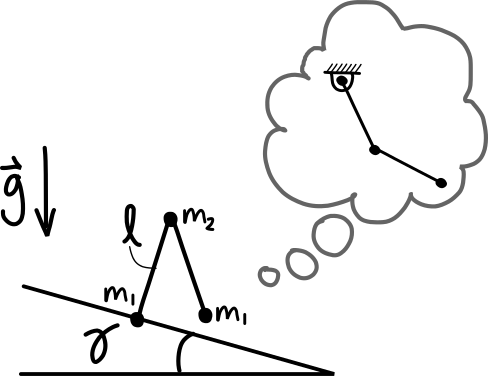
\includegraphics[width=0.6\textwidth]{Figures/SimplestWalkerPendulum} }


\maketitle

% \begin{centering}
% 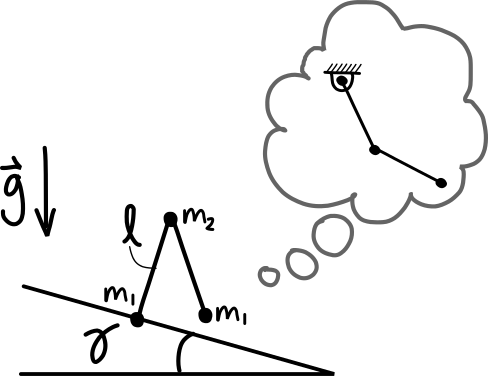
\includegraphics[width=0.1\textwidth]{Figures/SimplestWalkerPendulum}\par
% \end{centering}

% \end{titlepage}

\tableofcontents
\listoffigures

\chapter*{Preface}

This text is an expansion upon notes taken during TAM7960 entitled ``Legged locomotion of robots and animals
(Mechanics of terrestrial locomotion)'' at Cornell University, a course about mechanical models and empirical studies of legged terrestrial locomotion. The goal of the course is to shed light on the coordination, speed, energetics, and stability of locomotion in legged animals, especially humans. The notes were taken during the Spring 2010 offering of the course. This bulk of this text was written during the Fall 2010-Spring 2011 academic year.

This course and the material presented in this book present a variety of ways to model locomotion and analyze the stability and energy effectiveness of both actively and passively controlled versions of the various models. Miscellaneous topics arise throughout; some properties of electric motors, biological muscles, and central pattern generators will also be discussed in brief.

\chapter*{Work flow [temporary section]}

This section is a temporary section  to be used by the people working on the text. A more thorough documentation, include running meeting notes, etc. and a to-do list, are maintained as text files along with the .TEX source files. This provides perhaps a summary overview of such information.

\section*{Alan}

Working on sections:

\begin{itemize}
\item Introduction (needs some freshening up)
\item Motors and muscles ``complete"

\item Passive: stability-related sections
\begin{itemize}
\item Rimless wheel ``complete" (perhaps add a little stability information)
\item SLIP stability ``complete"
\item Simplest walker, ``complete" (perhaps add a little stability information)
\end{itemize}

\item Needed: Figure captions at the end of optimization ``complete"

\item Controlling ``complete" (CPG Section dropped for the first draft, still exists in the comments)
\item Energetics: optimal control ``complete''

\item Using Snopt (Appendix A) Could use some serious revision. I've somewhat forgotten how to use it. I could probably work through it again, unless someone with a good understanding of it could whip it up in a jiff... it would be pretty cool to have a nice detailed tutorial (with screenshots) in here on SNOPT or FMINCON (I think?) or other optimization packages, as they are pretty useful to this field (and in general). 

\end{itemize}

\section*{Chris}

It means that the writing is complete, it's been reviewed once, but is not complete simply because I'm sure it will need revision.

\begin{itemize}
\item Bits of introduction ``complete''
\item Modeling: ``complete'', with about 6-8 comments throughout, except for figure captions
\item Passive: dynamics-related sections

\begin{itemize}
\item rimless wheel: ``complete''
\item simplest walker: ``complete''
\end{itemize}

\item Energetics: requires elaboration/text on Figure 6.2 ParticleExplosion, Ruina's Rant, and about 4 comments/questions throughout ``mostly complete''
\item Optimization: energy optimization expeirments: ``complete''
\item Similarity: want to add more material from McMahon's book in relation to muscles, otherwise ``complete''.
\end{itemize}

\section*{Professor Ruina}

If Professor Ruina is interested, perhaps he could help with the Further Reading section, more immediately. It is likely that he could develop this section much quicker than either Alan or Chris.

% SECTIONS %%%%%%%%%%%%%%%%%%%%%%%%%%%%%%%%%%%%%%%%%
\chapter{Introduction}
\label{sec:Introduction}

This is an obvious TEST. 

On safari, Herb and Charlotte were capturing vivid images of the landscape and the beautiful animals among the bushes and wild grasses. A lone elephant roamed across the plains not sixty feet from them, sniffing the ground with its robust trunk, and making its way to the shade of a nearby tree. A silly image popped into Charlotte's mind. ``What if the elephant jumped into the tree?" she thought. To Herb, she repeated this question. Herb laughed, then puzzled, he thought about why the elephant could not jump as high as the gazelle bounding so effortlessly across the plains in the distance. ``The elephant seems ten times larger than that gazelle over there, shouldn't it be ten times as strong?" he asked. Charlotte pulled a book \cite{mcmahon84} out of her bag, and turned to the last chapter. Together, they read about similarity and scaling, and realized that while $mg \propto L^{3}$, $\sigma_{0, max}$ = constant.

Herb and Charlotte were fascinated by the possibility of making such inspiring discoveries from simple principles. In that very moment, they desired nothing more than they so powerfully desired a book that captures a smorgasboard of discoveries about animals and their graceful movement. This moment stayed with them until they were home, where Charlotte was in her darkroom developing pictures from the voyage. The pipes creaked in the darkness. A rat scurried across a stack of photos from a recent trip to an industrial robotics expo in Japan. She glanced in the direction of the sound. Honda's Asimo robot stared back at her from the photo at the top of the stack. She walked over to the table and placed a gentle hand on the picture, and cried. Finally, she knew...

\section{Philosophical Musings}

Things to talk about, possibly:
\begin{itemize}
\item Goal of locomotion
\item dry friction
\item skip wheels
\item animals vs robots
\item Radhakrishnan: locomotion is a balance of friction. in legged locomotion, we approximate rolling friction with no-slip contact: minimize frictional losses, kind of elegant. but nonetheless legged locomotors have a high cost of transport. this is because legged things are optimized for mobility, agility, and rough terrain. example is replacement of chariots with camels in middle east. we should include a plot from the Radhakrishnan paper as well.
\item passive locomotion
\item The story of this book: somebody is out there trying to make a real loco. what are the roadblocks to doing that? ROADBLOCKS
\item What is locomotion, and what is the objective of locomotion? Locomotion hints to the idea that the animal that is moving is trying to move from one location to another location. Dry friction, not linear viscous friction. want robot to move, not fall apart, translate. can use wheels, circumvent friction by lifting up legs. We must use friction, but frictional contact would mean energy loss? avoid dynamic friction.
\end{itemize}

\section{Locomotion}

What defines locomotion? Of course, it is a class of motion. It is the gainful movement from one location to another. However, riding a bicycle or driving a car is not a form of locomotion. Thus, locomotion implies self-propulsion. Locomotion comes in many forms. It is slithering, it is flying, it is swimming. If it is legged locomotion, it is walking, it is running, it is jogging, it is swimming, it is skipping, it is hopping, it is crawling, it is galloping, it is cantering, it is skating.

\section{Friction in Locomotion}

Locomotion often entails expending energy to travel at constant speed. This at first seems counter-intuitive, since energy should not be required to maintain an object's constant velocity. However, locomotion is riddled with friction.

Locomotion entails friction in two senses. Friction removes energy from a locomotive, either from the exterior rubbing against a fluid, or from the dissipative deformation of body tissue. Friction is also required to generate locomotion. Of course, animals must exert forces on their surrounding to propel themselves. Logically, this force is a contact force, and thus comes from friction. The friction between two rigid objects (e.g. a foot and the ground) can either be sliding friction or static friction. The invention of the wheel was particularly clever because a wheel circumvents the energy dissipation that arises from sliding friction and only uses static rolling friction. Equally clever, then, is legged animal locomotion: feet make non-sliding non-dissipative contact with the ground, they exert a static friction force against the ground. To actually move the body, the other leg(s) of the locomotive are lifted and moved forward while the one stationary leg pushes \cite{radhakrishnan98}. For all the cleverness is an equal amount of interesting dynamics to study. One interesting facet of the motion is the stability of such a clever system of movement.

\section{Control of Locomotion}
[We can take this section out but we just wanted to consider including some things from the conversation with Ruina that we had 3/2011. Ruina's previous viewpoint: passive was whole story, but passive robots are not as stable as their bio counterparts [Alan's meeting notes]

An inverted pendulum (in which the base is at the bottom rather than the top of the link) is unstable for most initial conditions. Locomotion can be termed stable if constant periodic movement can be achieved (i.e. the locomotive does not fall down after a few steps). It is instructive to study how stable locomotion can be achieved. Of course, all animals can achieve stable locomotion. A substantial question is what mechanisms provide this stability? Does the stability come from an active control process from the nervous system that ensures each leg is placed in the proper position? Alternatively, the stability could come from the pure mechanics of the locomotive. That is, the animal would be able to achieve stable motion even it did not have a brain. Such is the study of \emph{passive dynamics}, or \emph{passive control}, in which stability exists without control.

While a study of passive dynamics with regard to locomotion can provide some enlightening results, the study of active control is necessary to blah blah.

We can apply an understanding of locomotion in various engineering contexts such as robotics and biomechanics. This knowledge can inform the design of robots, of biomechanical equipment such as prosthetics, and can aid with the development of physical training regimens and surgical procedures. We are often interested, especially in robotics, in the energy cost of locomotion.

\section{A rose by any other name...}

\begin{itemize}
\item Locomotive: obvious reasons, but also means railcar
\item pedestrian: seems the most correct in terms of roots etc, but has weird associations with the public
\item legged thing: two words
\item LAR (legged robot and/or animal)
\item another latin combination?
\item robot: since we always simplify back to mechanics
\item legged mechanism
\end{itemize}

\section{Approaches to Understanding Legged Locomotion} %(notes page 1)
\label{sec:ApproachesToUnderstandingLeggedLocomotion}

There are three approaches we can take to understanding legged robots and animals. One is to assume no control, and just study the mechanics of locomotion. The second is to assume knowledge of the control schemes, and strive to optimize some locomotion parameter. This approach may involve something like optimization of hip torque or ankle torque to minimize energy use. The third approach is to analyze only the controller. The first and third methods are very closely related, as it is very difficult to discuss one without discussing the other. This book attempts to shed light on all three approaches, with a focus on energy use. 

Many successful walking robots already exist. Honda's Asimo is a capable home assistant that has been under development for nearly twenty years. BigDog, by Boston Dynamics, is a rugged battlefield assistant designed to carry heavy payloads for soldiers in variable terrain. These robots are very close to being able to do what the designers intended; however, one metric that escapes them and many other robots is energy effectiveness. These robots use significantly more power than their biological  counterparts. A human uses roughly 100 Watts of chemical energy when walking \cite{wilson04}. Legged robots like Honda's Asimo and BigDog by Boston Dynamics use anywhere from 2000 Watts to 18000 Watts of power. Honda's Asimo uses electric motors that are powered by batteries, while BigDog uses hydraulic actuators whose pump system is powered by a combustion engine \cite{needed}. As the field of legged robotics continues to grow, a better understanding of energy use will offer improvements in range and durability.

\section{Energy Effectiveness} %(notes page 2)
\label{sec:EnergyEffectiveness}
\index{energy effectiveness}

We would like some way to compare the effectiveness of legged robots. There are many qualitative ways to compare robots, such as a robotic arm's ability to manipulate its environment, or a mobile robot's ease of deployment in a battlefield. There are also ways to quantify a system's effectiveness; an automobile's energy use is typically cited in miles per gallon. We would like some way to cite energy use per distance traveled, but we would like it to be dimensionless so that we may equitably compare robots of different sizes. Given two robots that use equal amounts of energy to travel the same distance, the more useful robot is the one that can carry more mass. Adding mass to our comparison also conveniently makes the comparison dimensionless. Equation \ref{eq:CostOfTransport} defines the dimensionless cost of transport ($COT$):

\begin{equation}
COT = \frac{\mbox{energy spent}} {\mbox{mass}\cdot\mbox{gravity}\cdot\mbox{distance traveled}}=\frac{E}{mgd}
\label{eq:CostOfTransport}
\end{equation}
\index{cost of transport (COT)}

A particularly nonintuitive aspect of equation \ref{eq:CostOfTransport} is that the the $COT$ for animals that are not moving at all is infinity. This is because animals expend energy even when standing still, and none of this goes into center of mass movement \cite{radhakrishnan98}. Furthermore, the average $COT$ for legged animals is suspiciously high, considering that sliding or viscous friction does not play any significant role in the movement. Note that a non-zero $COT$ means that the locomotive must provide energy for even constant-speed movement on level ground. Where then is energy dissipated if not through external friction? During a walking gait, muscles contract and stretch. For the most part, the work that goes into contracting muscles is useful work. However, energy is lost in the so-called ``negative work'' that muscles ``perform'' when stretching under tension. This is elucidated in chapter \ref{sec:EnergeticsOfLocomotion}.

When creating robots that mimic biologically successful walking animals, it is important to examine the role of the $COT$ in legged animal evolution. The evolutionary pressure on the $COT$ is fairly evident: many animals consume energy as food to supply energy for homeostasis. The animal must also spend energy to find food and mates to reproduce, and a more biologically successful animal will be one that can find food and mates without expiring. An animal can be compared to a robot in that they both consume energy in some form, whether it be chemical or electric, and make use of that energy with a certain efficiency or effectiveness.


%%%%%%%%%%%%%%%%%%%%%%%%%%%%%%%%%%%%%%%%%%%%%%%%

\chapter{Properties of Motors and Muscles}
\label{sec:PropertiesOfMotorsAndMuscles}

Unfortunately, current technologies do not allow us to replicate the properties of muscles exactly. Muscles are strong and light, and can fit into extremely small spaces while still being able to deliver tremendous force. Muscles are a type of actuator, which may be defined as a system that converts energy from any form into motion (kinetic energy).The two most robust forms of man-made actuators in use today on legged robots are hydraulics and electric motors. Hydraulics are powerful, but they are extremely inefficient and can leak oil. Electric motors are far more efficient with energy, and thus are the main focus of actuation options in this text. This chapter starts with an introduction to the properties of electric motors and a discussion of their power consumption. The section on electric motors is followed by an introduction to human locomotive muscle properties, and how these muscles compare to electric motors.

\section{Motors} % (notes page 3-7)
\label{IntroductionToMotors}
\index{motors}

Generally speaking, using stored electricity to power electric actuators is extremely efficient. One \unit{Joule} of stored electric energy, in either a battery or capacitor, will deliver almost one \unit{Joule} of energy to an electric motor paired with the storage device. This is greatly different from combustion-driven actuators, for which the amount of energy stored in chemical bonds is approximately four times the amount of thermal energy that results from the combustion.
\par % trying Ruina's paragraph command
A basic configuration of an electric motor and a power supply is shown in figure \ref{fig:PowerSupplyAndMotor}. The voltage and current associated with the power supply are $V$ and $I$, respectively. The angular speed and torque provided by the motor are $\omega$ and $T$, respectively.

% FIGURE
\begin{figure}[h]		% h="here" t="top" b="bottom" p="separate page"
\begin{centering}
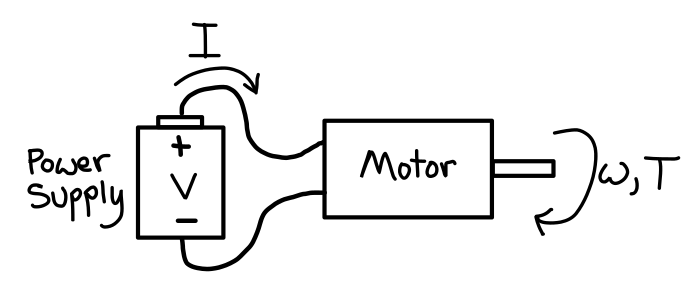
\includegraphics[width=0.5\textwidth]{Figures/PowerSupplyAndMotor}\par
\end{centering}
\caption[Diagram: Power Supply and Electric Motor]{Power supply and electric motor. The power supply provides $I$ Amperes of current at a potential difference of $V$ Volts. This creates $T$ Newton-meters of torque and spins the motor at $\omega$ radians per second.}
\label{fig:PowerSupplyAndMotor}
\end{figure}
%

We are interested in the relationships between $I$, $V$, $\omega$, and $T$. Given that we have four variables, we can choose one of them to control so that we are left with three equations that govern the other variables.

\subsection*{Power}
\label{sec:Power}

The power consumed and developed by the configuration shown in figure \ref{fig:PowerSupplyAndMotor} is described by the following equations:

\begin{equation}
P_{i}=P_{in} = \mbox{electric power into motor}= IV
\label{eq:PowerIn}
\end{equation}

\begin{equation}
P_{o}=P_{out} = \mbox{power motor exerts on environment} = T\omega
\label{eq:PowerOut}
\end{equation}

The fundamental restriction on electric motors is that there is always positive energy dissipation in the motor due to heat loss, and so power input from the battery is greater than power output by the motor. This holds true for many types of actuation systems, as it is nearly impossible to build a completely lossless, or ideal, machine or system. Figure \ref{fig:IdealPowerPlotSketch} demonstrates this fundamental restriction.

% FIGURE
\begin{figure}[h]		% h="here" t="top" b="bottom" p="separate page"
\begin{centering}
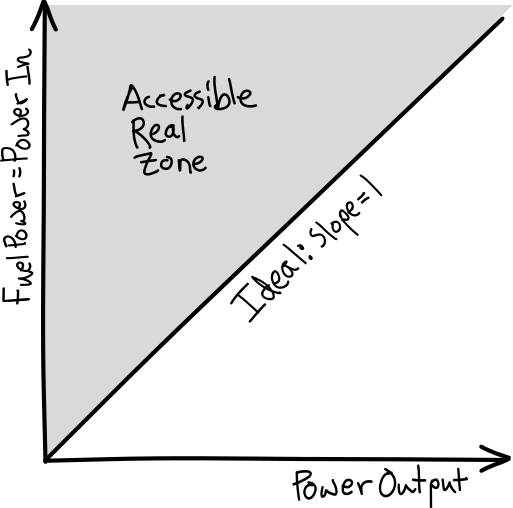
\includegraphics[width=0.5\textwidth]{Figures/IdealPowerPlotSketch}\par
\end{centering}
\caption[Plot: Power Conservation]{Fuel power input to a system vs. the power output by the system. An ideal system would produce as much power in the form of mechanical work as it consumes in chemical energy from fuel. The shaded area of this plot represents the performance levels attainable by real systems.}
\label{fig:IdealPowerPlotSketch}
\end{figure}
\index{power}

Imagine for one instant in time that $\omega$ is chosen or known. Perhaps this means that we want to set the speed at which a limb in a legged robot is rotating. This leaves the variables $T$, $V$, and $I$ to control in some way. If $V$ and $I$ are controlled, equations \ref{eq:PowerIn} and \ref{eq:PowerOut} can be combined in a power conservation equation:

\begin{equation}
IV = T\omega + I^{2} R
\label{eq:EnergyConservation}
\end{equation}

where the $I^{2}R$ term represents power dissipation from the internal resistance of the motor. Additionally, we can quantify the motor torque:

\begin{equation}
T = kI
\label{eq:MotorTorque}
\end{equation}

where $k$ is the motor torque constant, which has units of \unitfrac{Nm}{Amp}. Substitution of equation \ref{eq:MotorTorque} into equation \ref{eq:EnergyConservation}, gives the motor voltage law:

\begin{equation}
V = k\omega + IR
\label{eq:MotorVoltage}
\end{equation}

We think of equations \ref{eq:MotorTorque} and \ref{eq:MotorVoltage} as describing a motor that is controlled by a given voltage. So if given a voltage, say \unit[9]{Volts}, we would like to eliminate $I$ from these two equations so that we can see how the machine behaves. Manipulation yields:

\begin{equation}
V = k\omega + \frac{T}{k}R
\label{eq:MotorVoltage2}
\end{equation}

\begin{equation}
T = \frac{k}{R}V - \frac{k^2}{R}\omega
\label{eq:MotorTorque2}
\end{equation}

% FIGURE
\begin{figure}[h]		% h="here" t="top" b="bottom" p="separate page"
\begin{centering}
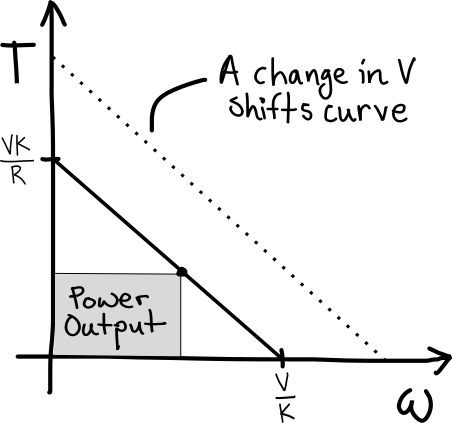
\includegraphics[width=0.4\textwidth]{Figures/MotorTorqueCurveSketch}\par
\end{centering}
\caption[Plot: Torque vs. Angular Speed for an Electric Motor]{Torque vs. angular speed for an electric motor. The relationship is linear, described by $T = \frac{k}{R}V - \frac{k^2}{R}\omega$ (equation \ref{eq:MotorTorque2}). Notice that $\frac{Vk}{R}$, the intersection of the curve and the torque axis, is directly proportional to $V$. The power developed by the motor, $T\omega$, is the area of the shaded rectangle for a given operating point.}
\label{fig:MotorTorqueCurveSketch}
\end{figure}
%

An important quantity to solve for is the free spinning angular rate $\omega_{f}$,

\begin{equation}
\omega_{f} = \frac{1}{k}V
\label{eq:FreeSpinningOmega}
\end{equation}

which is the speed at which the motor would rotate if there were no load on it. We can find the value of the motor torque constant in terms of $\omega_{f}$:

\begin{equation}
k = \frac{V}{\omega_{f}}
\label{eq:MotorTorqueConstant}
\end{equation}

where $k$ has units of \unitfrac{V}{rad/s}.

It's useful here to demonstrate the energy used by the motor:

\begin{equation}
P_{i} = VI = V\frac{T}{k} = \frac{V}{k}\left(\frac{k}{R}V - \frac{k^2}{R}\omega\right)
\label{eq:MotorPowerUse}
\end{equation}

Equation \ref{eq:MotorPowerUse} describes the power consumed by the motor, which is equal to the power supplied by the battery. This power is called the input power. This power relationship is shown in figure \ref{fig:PowerVsOmega} as a straight line, where the curved line is the output power, $P_{o}$:

\begin{equation}
P_{o} = T\omega= \left(\frac{k}{R}V - \frac{k^2}{R}\omega\right)\omega
\label{eq:MotorPowerOutput}
\end{equation}

Given the input and output power, we can calculate the motor efficiency.

\begin{equation}
\mbox{efficiency} = \frac{P_{o}}{P_{i}}
\label{eq:MotorEfficiency}
\end{equation}

At peak power, $\omega = \frac{\omega_{f}}{2}$ and the efficiency therefore equals 50\%. The peak efficiency is close to 1 when $\omega$ approaches $\omega_{f}$. The efficiency is shown in figure \ref{fig:MotorEfficiency}.

% FIGURE
\begin{figure}[h]		% h="here" t="top" b="bottom" p="separate page"
\begin{center}
 \subfloat[]{\label{fig:PowerVsOmega}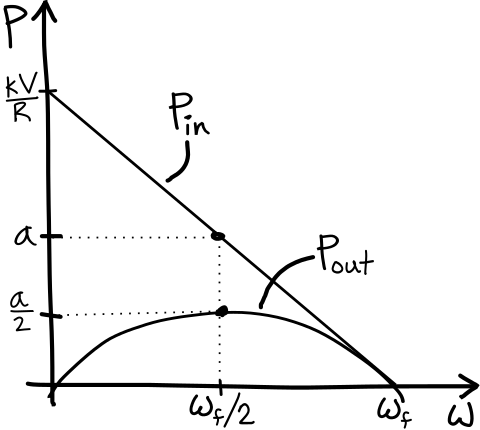
\includegraphics[width=0.38\textwidth]{Figures/PowerVsOmega}} \hspace{0.05\textwidth}%
 \subfloat[]{\label{fig:MotorEfficiency}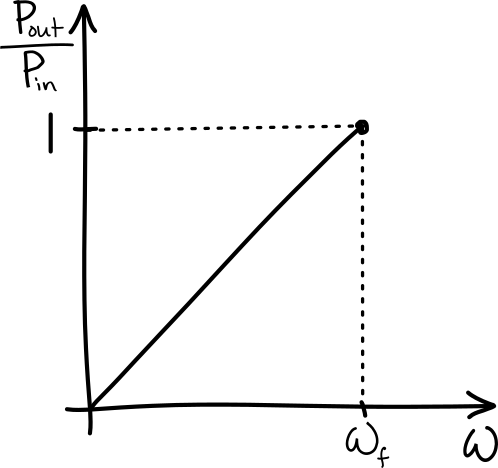
\includegraphics[width=0.33\textwidth]{Figures/MotorEfficiency}}
\end{center}
\caption[Plot: Electric Motor Power and Efficiency vs. $\omega$.] {(a) Output motor power vs. rotational speed, $\omega$. This plot shows equations \ref{eq:MotorPowerOutput} and \ref{eq:MotorPowerUse} on the same axis. The rotational speed that produces the greatest power output is half of the free spinning rotational speed of the motor. The required power drawn from the battery at this speed is twice the developed power, as indicated by the points labeled $a$ and $a/2$ on the P axis.  (b) Electric motor efficiency vs. $\omega$. An electric motor is most efficient when it is allowed to spin at its free spinning rotational speed. However, as shown in figure \ref{fig:PowerVsOmega}, the motor produces no power when it spins at its free spinning rotational speed.}
\label{fig:MotorPowerAndEfficiency}
\end{figure}
%

With our basic motor model, we can compare plots of various quantities, as in figure \ref{fig:FourMotorCurves}.

% FIGURE
\begin{figure}[h]		% h="here" t="top" b="bottom" p="separate page"
\begin{centering}
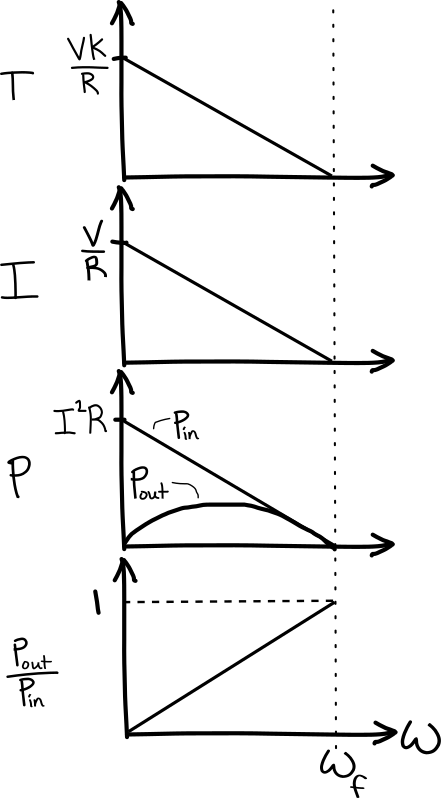
\includegraphics[width=0.35\textwidth]{Figures/FourMotorCurves}\par
\end{centering}
\caption[Plot: A Comparison of Four Motor Curves vs. $\omega$]{A comparison of motor torque, current, power, and efficiency. The torque, $T$, is a linear function of $\omega$, as is the current, $I$. The current function is simply the torque function scaled by $k$. The bottom two plots are the power and efficiency curves from figure \ref{fig:MotorPowerAndEfficiency}, shown again to emphasize that the motor produces no torque and draws no current at its free spinning rotational speed.}
\label{fig:FourMotorCurves}
\end{figure}
%

Running a motor at a low $\omega$ is not very efficient, but running a motor near free speed is very efficient. Given any motor, we can increase $V$ arbitrarily and get any power at any efficiency we choose. However, as we increase $V$ at a fixed efficiency, we also inadvertently must change $\omega$, which may not be desirable. The solution to this problem is to convert nearly free-speed rotation at the motor to a rotational speed of our choosing at our application point, e.g. at the limb of a legged robot. This scaling can be accomplished with gearboxes. A gearbox is a passive box that ideally preserves input power, or: $P_{in}=P_{out}$.

\begin{equation}
T_{in}\omega_{in} = T_{out}\omega_{out}
\label{eq:GearboxExample}
\end{equation}

% FIGURE
\begin{figure}[h]		% h="here" t="top" b="bottom" p="separate page"
\begin{centering}
 \subfloat[]{\label{fig:GearboxExample}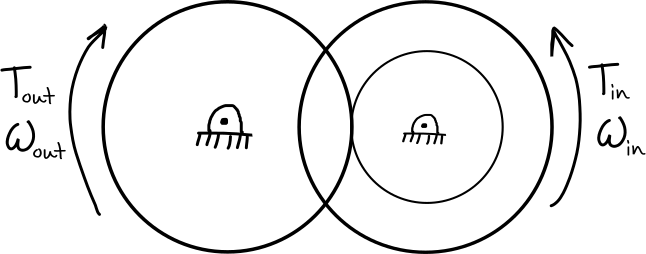
\includegraphics[width=0.5\textwidth]{Figures/GearboxExample}} \hspace{0.1\textwidth}%
 \subfloat[]{\label{fig:PulleyExample}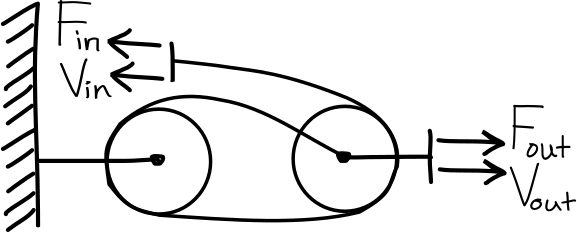
\includegraphics[width=0.4\textwidth]{Figures/PulleyExample}}
\end{centering}
\caption[Diagram: Force Amplification with Gearbox and Pulley Systems]{(a) A simple gear system. In this case, the input torque $T_{in}$ is amplified, while the input rotational speed $\omega_{in}$ is reduced ($T_{out}>T_{in}$ and $\omega_{out}<\omega_{in}$). (b) A simple pulley system. In this case, the output force is amplified, while the output velocity is reduced ($F_{out}>F_{in}$ and $V_{out}<V_{in}$). For both systems, power is conserved.}
\label{fig:GearboxAndPulleyExample}
\end{figure}
%

One drawback of gearboxes is that amplification of force (or equivalently torque) comes with a reduction in velocity. This is best illustrated with a pulley example, as in figure \ref{fig:PulleyExample}.

\begin{equation}
F_{in}v_{in} = F_{out}v_{out}
\label{eq:PulleyExample}
\end{equation}

One of the key problems in robotics is how to appropriately size a gearbox. The key equations for this problem are shown in equation \ref{eq:MotorAndGearbox}.

\begin{align}
T_{out} &=GT_{in} \notag \\
\omega_{out} &=\omega_{in}/G \notag \\
T_{in}\omega_{in}&=T_{out}\omega_{out}
\label{eq:MotorAndGearbox}
\end{align}

where $G$ is the gear ratio. These equations \ref{eq:MotorAndGearbox} neglect the presence of friction in the gearbox.

% FIGURE
\begin{figure}[h]		% h="here" t="top" b="bottom" p="separate page"
\begin{centering}
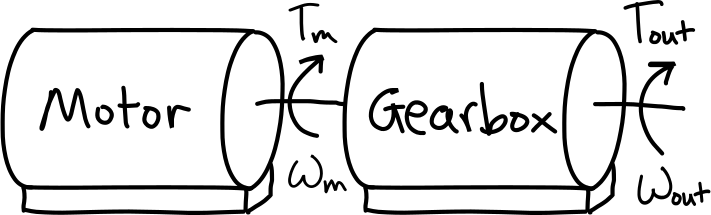
\includegraphics[width=0.5\textwidth]{Figures/MotorAndGearbox}\par
\end{centering}
\caption[Diagram: Motor Connected to a Gearbox]{A motor connected to a gearbox. The motor develops a torque $T_{m}$ and rotational speed $\omega_{m}$, which the gearbox converts into an output torque $T_{out}$ and rotational speed $\omega_{out}$. An ideal gearbox is frictionless and conserves power; the relationship between the torques and rotational speeds is described by equation \ref{eq:MotorAndGearbox}.}
\label{fig:MotorAndGearbox}
\end{figure}
%

Given any motor, $k, R$ and any efficiency, say 98\%, any power output, $P_{out}=\unit[50]{W}$, and any $\omega=\unitfrac[4]{rev}{s}$, we can pick $V$ and $G$ to do the job. However, there are some practical considerations to be aware of when choosing $V$ and $G$ for real systems.  

\begin{itemize}

\item \textbf{Motor melting.} An electric motor generates heat during operation, and can only dissipate so much heat before destroying itself.
\item \textbf{Sparking danger.} A large V could create sparking across wire leads or brush tips within the motor and cause damage to components in the motor or in the circuit that powers the motor.
\item \textbf{Real gears have friction.} The bigger the gear reduction, the more friction there is in the gearbox.
\item \textbf{Inertia.} Reflected inertia is proportional to $J_{shaft}G^{2}$.

\end{itemize}

From some of these considerations, we can build a more complete motor law.

\begin{equation}
T_{m}=kI-J\dot{\omega}_{m}
\label{eq:CompleteMotorLaw1}
\end{equation}

where the subscript $m$ denotes quantites related to the motor itself as opposed to quantities at the output of a gearbox, and $kI=T_{e}$. The voltage across the motor is

\begin{equation}
V=k\omega_{m}+IR+L\dot{I}
\label{eq:CompleteMotorLaw2}
\end{equation}

where $L$ is the inductance of the motor. The term $L\dot{I}$ allows for pulse width modulation (PWM) control of the motor. The torque provided at the output of the gearbox has the form

\begin{equation}
T_{out}=GC_{1}T_{in}-C_{2}\omega-C_{3}\frac{\omega}{|\omega|}
\label{eq:CompleteMotorLaw4}
\end{equation}

where

\begin{equation}
C_{1}=\frac{1}{1+\mu \cdot \mbox{sign}\left(T_{in}\omega_{in}\right)}
\label{eq:CompleteMotorLaw5}
\end{equation}

and $C_{2}\omega$ represents viscous friction and $C_{3}\frac{\omega}{|\omega|}$ represents dry friction. If $\mu > 1$, non-backdriveable, or if efficiency forward $< 0.5$ (50\%).

% FIGURE
\begin{figure}[htb]		% h="here" t="top" b="bottom" p="separate page"
\begin{centering}
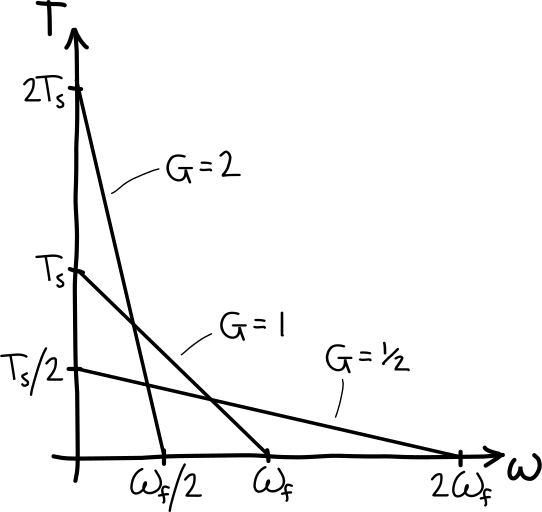
\includegraphics[width=0.4\textwidth]{Figures/GearboxCurves}\par
\end{centering}
\caption[Plot: Gearbox Torque Curves]{Gearbox torque curves. These curves are a modified version of those shown in figure \ref{fig:MotorTorqueCurveSketch}, but for different values of the gear ratio $G$. The greater the gear ratio, the greater the output torque and the smaller the output rotational speed.}
\label{fig:GearboxCurves}
\end{figure}
%

It is desireble to know the input power required to obtain a particular output power. If friction in the motor and gearbox are ignored, then the input power is a parabolic function of output power that also depends on $\omega$, k, R, and G (equation \ref{eq:GearboxPowerCurves}, figure \ref{fig:GearboxPowerCurves}). In equation \ref{eq:GearboxPowerCurves}, note that a gearbox amplifies the motor torque constant by the gear ratio. A few observations can be made from figure \ref{fig:GearboxPowerCurves}. Logically, less input power is required for a given output power as the motor resistance decreases. For low output powers, the current going through the motor is small and so the power loss from internal resistance is low and the motor is nearly 100\% efficient. 

\begin{equation}
P_{in}=P_{out}+P_{out}^{2}\frac{R}{(Gk)^{2}}
\label{eq:GearboxPowerCurves}
\end{equation}


% FIGURE
\begin{figure}[htb]		% h="here" t="top" b="bottom" p="separate page"
\begin{centering}
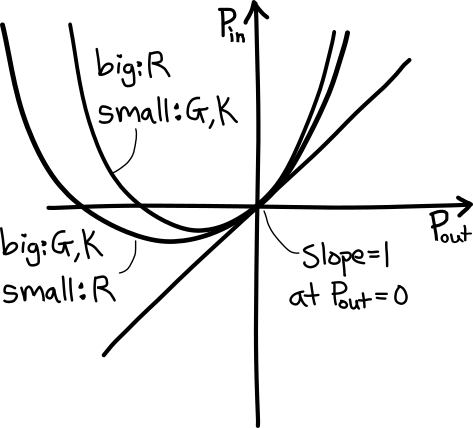
\includegraphics[width=0.4\textwidth]{Figures/GearboxPowerCurves}\par
\end{centering}
\caption[Plot: Gearbox Power Curves]{Gearbox power curves. A plot of equation \ref{eq:GearboxPowerCurves} for two different values of $R/(Gk)^2$. The curve is a parabola that intersects the origin with a slope of 1.}
\label{fig:GearboxPowerCurves}
\end{figure}
%

%%%%%%%%%%%%%%%%%%%%%%%%%%%%%%%%%%%%%%%%%%%%%%%%%

\section{Introduction to Muscles} % (notes page 7-9, 66)
\label{sec:IntroductionToMuscles}
\index{muscles}

This section is meant to serve as only a brief introduction to muscles and the mechanisms that make them work. Only a basic understanding of muscles is needed to understand the rest of the material in this book. The information presented here is a collection of bits and pieces. For a more detailed explanation of the topics discussed here, the reader should consult a basic introductory biology textbook. 

The main topic of concern for this field of study is energy use. This section introduces indirect calorimetry, metabolic efficiency, peak power consumption, the effect of slope on energy consumption, and the basic mechanisms that allow the body to move, such as muscle geometry on both a macroscopic and microscopic scale. 

\subsection{Muscle Geometry and Mechanisms}

Figure \ref{fig:HumanLeg} demonstrates some terminology that is commonly used when referring to muscles. Figure \ref{fig:HumanLeg} shows only the calf muscle of a human leg. The muscle is attached securely to the bone by tendons. Each end of the muscle is attached to different bones in the leg so that when the muscle contracts, movement is produced in the joint that connects the two bones. The calf muscle is attached to the back of the foot by the achilles tendon, and to the top of the lower leg (the tibia) just below the knee. The point where the calf attaches to the foot is called the insertion, and the point where it attaches to the tibia is called the origin. When the calf muscle contracts, a person's ankle bends and points the tip of the foot away from the rest of the leg. Since the calf muscle is located on the tibia itself, the foot is considered to be moving relative to the tibia. This relationship defines what we call the insertion and the origin; the insertion is usually the connection point on the part of the body that is moving relative to where the muscle is located. 

Animal muscles can only work in tension, so muscles must always come in pairs. To point a foot towards the knee, a muscle other than the calf muscle must contract. These pairs of muscles are called antagonistic because they pull in opposite directions of one another.  Figure \ref{fig:HumanLeg} does not show the muscle that completes the antagonistic pair with the calf muscle. 

% FIGURE
\begin{figure}[htb]		% h="here" t="top" b="bottom" p="separate page"
\begin{centering}
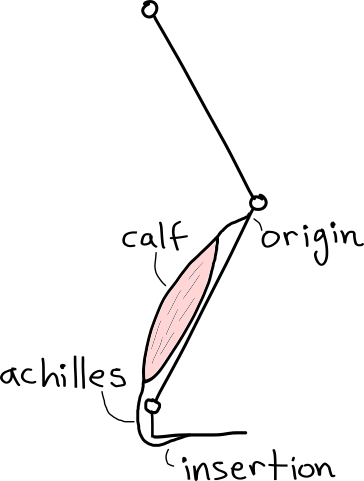
\includegraphics[width=0.3\textwidth]{Figures/HumanLeg}\par
\end{centering}
\caption[Diagram: Simple Human Leg Muscle Terminology]{Simple human leg muscle terminology. Only the calf muscle is shown, attached to bone by tendons. The origin is the point where the tendon attaches to the bone that does not move as a result of muscle contraction. The insertion is the point where the tendon attaches to the bone that is actuated by the muscle. On a human leg, the calf muscle insertion tendon is called the achilles tendon.}
\label{fig:HumanLeg}
\end{figure}
%

The tendons that connect a muscle to bone cannot actively contract. Tendons \index{tendons} are passive elastic connections from the muscle to the bone. They are only slightly elastic, but nearly perfectly so. Tendons have a small associated hysteresis \index{tendons!hysteresis} when lengthening and shortening, but this hysteresis only causes approximately 10\% of the work done during lengthening to be lost during shortening. In this regard, tendons are very similar to springs \index{tendons!springs}, and are sometimes modeled as such. Modern robots designed to replicate human locomotion sometimes incorporate stiff springs in series with an actuated cable to approximate a human muscle. 

% FIGURE
\begin{figure}[htb]		% h="here" t="top" b="bottom" p="separate page"
\begin{centering}
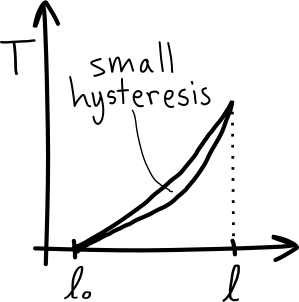
\includegraphics[width=0.25\textwidth]{Figures/TendonTensionPlot}\par
\end{centering}
\caption[Plot: Tension vs. Length for a Human Tendon]{Tension vs. Length for a human tendon. Tendons behave similarly to springs; however, there is a small hysteresis that occurs when loading and unloading tendons. The hysteresis loop forms clockwise; the tendon withstands greater force as it is being lengthened.}
\label{fig:TendonTensionPlot}
\end{figure}
%

Active contraction in muscles is the result of a microscopic structure called a sarcomere. The sarcomere is the basic functional unit responsible for muscle contraction; one muscle is made up of thousands of sarcomeres. Sarcomeres are composed of myosin and actin, intertwined as shown in figure \ref{fig:Sarcomere}. The strands, or filaments, of myosin and actin are connected by myosin heads that act as small levers. The myosin heads are part of the myson filaments, but temporarily connect to the actin filaments. When the two filaments are temporarily connected, the myosin heads bend in one direction, release, and bend back to stick to the actin again and repeat the action. This motion incrementally pulls the filaments of actin past the filaments of myosin, and the total width of the sarcomere shortens. The figure shows that there is a maximum possible contraction for any given sarcomere, and thus a maximum possible contraction for a given muscle. 

% FIGURE
\begin{figure}[htb]		% h="here" t="top" b="bottom" p="separate page"
\begin{centering}
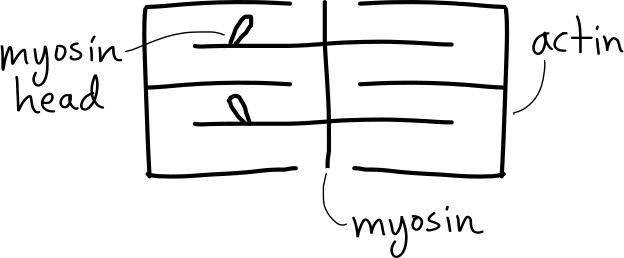
\includegraphics[width=0.35\textwidth]{Figures/Sarcomere}\par
\end{centering}
\caption[Diagram: A Sarcomere]{A sarcomere. The sarcomere is the basic functional unit responsible for muscle contraction. They are composed of myosin and actin, intertwined as shown and connected by myosin heads that act as small levers. The myosin heads connect to the actin, bend in one direction, release, and bend back to repeat the action. This motion incrementally pulls the actin closer to the myosin.}
\label{fig:Sarcomere}
\end{figure}
%

Muscles are active motors, and subsequently need fuel to operate. This fuel originally comes from caloric intake, but is spent at the muscle as a chemical called ATP (adenosine triphosphate). Only 25\% of total fuel intake goes to actual work performed by a muscle. Nearly 50\% of fuel intake is used to convert energy stored as fat to useable ATP. The process of converting fats and starches to ATP is called metabolism. Another 50\% of fuel intake is spent in the sarcomeres, converting ATP to mechanical work. Within the sarcomere, ATP and calcium ions work together to make the grab-and-release cycle happen. Calcium levels control the process, and the calcium is delivered to the muscle through a sheath that surrounds the muscle itself.

It is possible to externally stimulate muscles and force joints to actuate by applying an electric current or field to the muscle. This can be done even through the skin because an electric field can penetrate the skin and muscle tissue and cause the charged calcium ions to leave the sheath and enter the muscle. This external stimulation bypasses the normal biological process, which relies on neurons to deliver a weak electric signal to release the calcium into the muscles. 


\subsection{Muscle Energy Use}

In order to measure the energy used by muscles for locomotion we can test individual muscles for their strength or we can analyze a human as a black box that consumes energy through metabolic processes and then outputs work through locomotion. 

\subsubsection*{Indirect calorimetry}

One such black box method is called Indirect Calorimetry. This method measures the oxygen entering and carbon dioxide leaving the body, and assumes that the intermediate chemical reaction is equivalent to combustion (``burning" food). By measuring oxygen and carbon dioxide in this way, it is possible to indirectly measure the amount of food (input energy) that is used as work for locomotion. This measurement is commonly quantified by the volume of oxygen, or ``$V_{O_2}$.", inhaled. The ratio of carbon dioxide to oxygen can provide the ratio of starch to fat that is burned.

% FIGURE
\begin{figure}[htb]		% h="here" t="top" b="bottom" p="separate page"
\begin{centering}
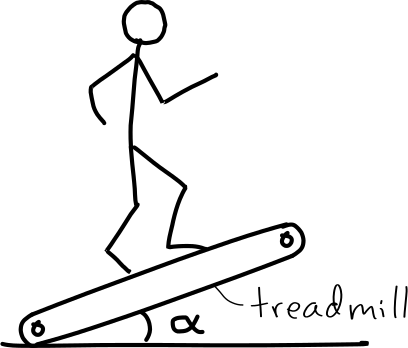
\includegraphics[width=0.35\textwidth]{Figures/Treadmill}\par
\end{centering}
\caption[Diagram: Treadmill Experiment Arrangement]{Treadmill experiment arrangement. This arrangement can be used to measure the relationship between energy use and the angle $\alpha$ of a walking surface. Increasing $\alpha$ effectively increases the amount of output work the human must perform.}
\label{fig:Treadmill}
\end{figure}
%

With a treadmill setup like the one in figure \ref{fig:Treadmill}, measurements of oxygen intake can be used to learn about the efficiency of human walking as is shown in figure \ref{fig:MetabolicCost}. As we may have garnered from experience, increasing $\alpha$ increases the amount of work the human must output to remain on the treadmill. The output work (a greater $\alpha$) requires the human to burn a certain amount of food calories (energy). This amount of energy that must be burned is the metabolic cost of locomotion. By varying $\alpha$, one can obtain different levels of output work and measure through $V_{O_2}$ the corresponding metabolic cost of that work.

% FIGURE
\begin{figure}[htb]		% h="here" t="top" b="bottom" p="separate page"
\begin{centering}
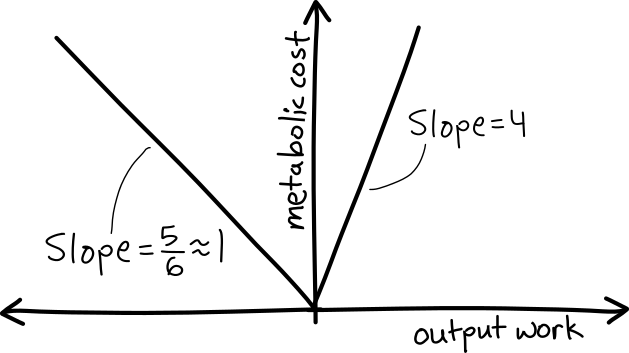
\includegraphics[width=0.5\textwidth]{Figures/MetabolicCost}\par
\end{centering}
\caption[Plot: The Metabolic Cost of Walking on a Hill]{The metabolic cost of walking on a hill.  When walking uphill, a human must input as metabolic cost approximately 4 times as much energy as the minimum energy required to move their mass uphill. Note that there is a metabolic cost for a human to walk downhill, even though a ball does not need to input energy to roll down a hill. A human must input as metabolic cost approximately 5/6 of the energy that would be created by a ball with the human's mass rolling down the hill.}
\label{fig:MetabolicCost}
\end{figure}
%

When walking uphill, the metabolic cost of locomotion associated with climbing a hill a certain distance is approximately 4 times the potential energy gained by traversing that distance. This provides an energy efficiency of $1/4 = 25\%$. For a lossless mechanism, the metabolic cost of traversing a distance up a hill would be equivalent to the output work, giving a slope of 1 in figure \ref{fig:MetabolicCost}. This is due to energy losses in converting caloric intake to fats and starches and converting those fuels into mechanical work. When walking downhill, the theoretical mechanical output work is actually negative, but humans are incapable of recovering that energy as they walk downhill. Humans still have to use metabolic energy to prevent themselves from essentially falling or tumbling downhill. The amount of energy a person spends trying to check their speed going downhill is nearly equal to the amount of energy they would gain if they were to just roll downhill. In general, the greater the incline, the more tiring it is to walk up it. The metabolic cost is linear with increases in the steepness of the slope. Also, the greater the incline, the more tiring it is to walk down it, but walking down a given incline is easier than walking up it. 

% Here's a little bit that I don't understand (AVA 20110814):

%The simplest estimate of energy cost of using muscle:
%
%\begin{align}
%P_{cost} &= C_{1}|P| \mbox{ for } P > 0\notag \\
%P_{cost} &= C_{2}|P| \mbox{ for } P < 0
%\label{eq:MetabolicCost}
%\end{align}
%
%where $C_{1}\approx0.25$ and $C_{2}\approx0.05$.

\subsubsection*{Individual muscles}

In order to determine the maximum energy or power that a muscle can exert, we need to introduce muscle strength and muscle stress.
\par
The idea that walking downhill is easier than walking uphill (for a given incline) can be observed on a smaller scale, at the muscular level. An individual muscle is also better at lowering a mass than raising a mass. Figure \ref{fig:LiftingVsLowering} shows that the amount of weight that a muscles can lower (negative work) is greater than the amount of weight that a muscle can lift (positive work). Such data is determined experimentally. The isometric strength of a muscle $T_{0}$ is how much force a muscle can provide if its length is kept fixed. Note here that the term strength is not denoting a maximum stress of a material as it does in mechanics, but a maximum force that can be exerted. The force a muscle can provide when lengthening is approximately 1.7 times the muscle's isometric strength. Also, a muscle in contraction provides less force the faster it contracts.

% FIGURE
\begin{figure}[htb]		% h="here" t="top" b="bottom" p="separate page"
\begin{centering}
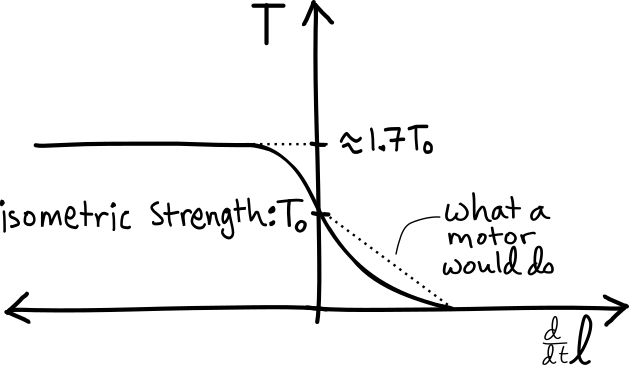
\includegraphics[width=0.5\textwidth]{Figures/LiftingVsLowering}\par
\end{centering}
\caption[Plot: Muscle Tension vs. Length Rate of Change]{Muscle tension vs. length rate of change. A muscle is capable of lowering more than it can lift. The isometric strength of a muscle $T_{0}$ describes how much force a muscle can provide with no change in length. The force a muscle can provide when lengthening is approximately 1.7 times the isometric muscle strength. A muscle in contraction provides less force the faster it contracts.}
\label{fig:LiftingVsLowering}
\end{figure}
%

Figure \ref{fig:PeakMuscleStress} is essentially the same as Figure \ref{fig:LiftingVsLowering}, except that the quantities on both axes have been normalized as is typically done in mechanics.  The isometric strength of a muscle is directly related to the peak muscle stress by a factor of the cross-sectional area of the muscle. In reality, a muscle will change cross-sectional area as it contracts, and the idea of ``stress" is only meant as a useful guide for thinking. The peak muscle stress is kind of like a muscle yield strength, except instead of yielding, the muscle simply cannot hold any more load and begins to release. For most muscles, this peak muscle stress is approximately equal to 0.1\% of the yield strength of steel.

% FIGURE
\begin{figure}[htb]		% h="here" t="top" b="bottom" p="separate page"
\begin{centering}
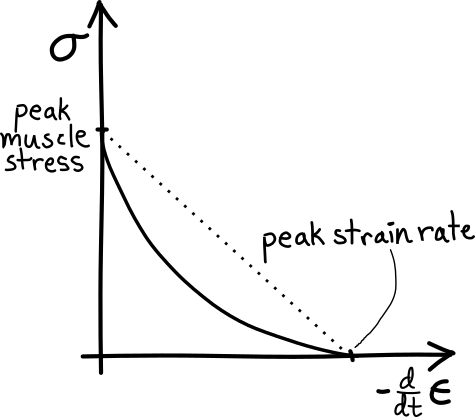
\includegraphics[width=0.4\textwidth]{Figures/PeakMuscleStress}\par
\end{centering}
\caption[Plot: Muscle Stress vs. Strain Rate]{Muscle stress vs. strain rate. The peak muscle stress can be thought of as a kind of yield strength, except instead of yielding the muscle simply cannot hold any more load and begins to release.}
\label{fig:PeakMuscleStress}
\end{figure}
%

\begin{equation}
\sigma_{peak} \approx 200 kPa
\label{eq:PeakMuscleStress1}
\end{equation}

Muscles can only operate at points on the curve in figure \ref{fig:PeakMuscleStress}, but there is bound to be an operation point at which the muscle is producing the most power it can produce. This point is at the coordinates ($\dot{\epsilon}_{peak}/3, \sigma_{peak}/3$).

\begin{equation}
\mbox{Peak Power} \approx \left(\frac{1}{3} \dot{\epsilon}_{peak}\right)\left(\frac{1}{3} \sigma_{peak}\right)
\label{eq:PeakMuscleStress2}
\end{equation}

Equation \ref{eq:PeakMuscleStress3} is a quick back-of-the-envelope calculation that shows how much power a kilogram of muscle develops. The calculation assumes a peak strain rate of $\unit[5]{s^{-1}}$, the peak muscle stress from equation \ref{eq:PeakMuscleStress1}, and a muscle density approximately that of water.

\begin{equation}
\mbox{Power/Mass} \approx \frac{\unit[5]{s^{-1}}}{3}\left(\frac{\unit[200000]{N/m^2}}{3}\right)\frac{1}{\unit[1000]{kg/m}} \approx \unit[200]{W/kg}
\label{eq:PeakMuscleStress3}
\end{equation}

In reality, the peak power is closer to \unit[50]{W/kg}. The best electric motors have a peak power/mass of approximately \unit[4000]{W/kg}, but typically they are only around \unit[200]{W/kg}. For most situations, this means that the power density of electric motors is only slightly better than that of muscle (by a factor of 4). This comparison neglects any considerations made for battery or power supply weight that might be needed to power an electric motor. 



%%%%%%%%%%%%%%%%%%%%%%%%%%%%%%%%%%%%%%%%%%%%%%%%

\chapter{Modeling Legged Locomotion}
\label{sec:ModelingLeggedLocomotion}
\index{models of locomotion}

We develop models of locomotion in order to understand various aspects of the dynamics of the motion of locomotives. The objective of a model of locomotion is to describe the kinematic structure of legs (links, joints, supports, and actuators) and the nature of the loading on this structure or the energy transfer (e.g. impact loading, spring energy), in a manner that makes sense for a particular model, that can realistically represent the forces and motions that occur in actual locomotion. Accordingly, a model of locomotion includes illustrations of its kinematic structure and equations that describe force interactions or energy transfer that correspond to the behavior of the kinematic structure in a manner that makes sense for a particular model. We can compare some models to each other by using the metric of metabolic cost of transport\index{metabolic cost}. The description of the models is not strictly motivated by such goals though. At various points, some interesting expressions are developed for their own sake.

This chapter first presents the equations of motion in the notation of this text, and then describes three models of locomotion. In order of increasing complexity these are the point mass model, the collisional model, and the spring-loaded inverted pendulum (SLIP) model.

\section{Equations of Motion} %(notes page 40-43)
\label{sec:EquationsOfMotion}
\index{equations of motion}
\index{motion, equations of}

The fundamental equations of dynamics are provided here without derivation. Such derivations can be found in any introductory dynamics textbook. The equations here are presented to provide the notation and symbols that are used throughout the text, as well as to clarify the equations of motion for multi-object systems. The locomotion models in this text consist of only point masses, and so the rigid object formulation of the equations of motion is not presented.

The terms particle and point mass are used interchangeably. The vectors here are vectors in two dimensional space, as all of the models are two-dimensional. The vector $\vr$ denotes a position in space, the vector $\vv$ denotes the velocity of a position, and the vector $\va$ denotes the acceleration of a position. The center of mass of an object is denoted as $G$. The notation $G/C$ reads as ``the center of mass with respect to point C''. If a quantity is not denoted as being ``with respect to'' a point (e.g. $\vr_{i}$), then the point is assumed to be defined with respect to the origin of the system $O$.

\subsubsection*{A single point mass}
For a point mass\index{point mass}, the equations of motion are simple. Only linear momentum balance (LMB)\index{linear momentum balance} and energy balance are relevant, since a particle cannot rotate. The linear momentum of a particle is

\begin{equation}
\vL = m\vv
\end{equation}

Linear momentum balance, or Newton's second law, for a particle states that

\begin{align}
\sum_{i} \vF_{i} &= \vLdot \\
&= m \va
\end{align}

where $\vF_{i}$ is the $i$-th contact or body force acting on a particle with mass $m$. The sum of the vector forces gives rise to the particle's acceleration $\va$. The energy of a particle $E$, neglecting friction, is given by

\begin{align}
E &= \KE + \PE \\
&= \frac{1}{2}mv^{2} + mgh
\end{align}

\subsubsection*{Collection of point masses}
Most of the models in this text involve multiple point masses. For a system of point masses such as in the general example of figure \ref{fig:EnergyAccounting} the center of mass relative to an arbitrary point $C$ is

% FIGURE
\begin{figure}[h]		% h="here" t="top" b="bottom" p="separate page"
\begin{centering}
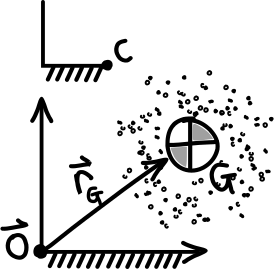
\includegraphics[width=0.3\textwidth]{Figures/EnergyAccounting}\par
\end{centering}
\caption[Diagram: Energy Accounting]{Energy accounting. This figure shows how to find the center of mass for a general system of point masses. The center of mass can be be described in any reference frame. [chris: why is this figure called Energy Accounting?]}
\label{fig:EnergyAccounting}
\end{figure}
%

\begin{equation}
\vr_{G/C} = \frac{\sum \vr_{i/C} m_{i}}{\sum m_{i}}
\label{eq:CenterOfMass1}
\end{equation}

Upon simple rearranging, equation \ref{eq:CenterOfMass1} yields 

\begin{equation}
m_{tot} \vr_{G/C} = \sum_{i} \vr_{i/C} m_{i}
\label{eq:CenterofMass2}
\end{equation}

where $m_{tot} = \sum m_{i}$. If equation \ref{eq:CenterOfMass1} is differentiated with respect to time, it relates the velocity of the system's center of mass to the velocities of the objects that compose the system. For a system of particles, the linear momentum is the sum of the linear momentum of each particle.

\begin{equation}
\vL = \sum_{i} m_{i} \vv_{i} = m_{tot} \vv_{G}
\end{equation}

Proceeding naturally, the linear momentum balance for a system of point masses

\begin{equation}
\sum_{i} \vF_{i}^{ext} = \vLdot
\end{equation}

Only external forces are relevant for LMB. Internal forces are defined as being between two masses within the system, and Newton's second law requires these forces to cancel each other. The external forces can arise from fields such as gravity, or contact with a surface or a mass that is not part of the system.

The angular momentum of the system with respect to a point $C$ is defined as

\begin{equation}
\vHC = \sum_{i} \vr_{i/C} \times m_{i} \vv_{i}
\end{equation}

For the purposes of this text, the point $C$ is fixed in space. This requirement allows the simplification of time derivatives of the angular momentum. The positions and velocities can be written relative to the center of mass of the system, yielding

\begin{equation}
\vHC = \sum_{i} (\vr_{i/G} + \vr_{G/C}) \times (\vv_{i/G} + \vv_{G/C}) m_{i}
\end{equation}

When the terms in this equation are expanded, the angular momentum is

\begin{align}
\vHC &= \sum_{i} \vr_{i/G} \times \vv_{i/G} m_{i} + \vr_{G/C} \times \vv_{G/C} \sum_{i} m_{i} \notag \\
& + \sum_{i} \vr_{i/G} m_{i} \times \vv_{G/C} + \vr_{G/C} \times \sum_{i} \vv_{i/G} m_{i}
\label{eq:AMBSystem}
\end{align}

Based on the definition of the center of mass, the summation $\sum \vr_{i/G}m_{i}$ and its derivatives are zero. As a result, the second two terms of equation \ref{eq:AMBSystem} are zero. The first term in the expansion is a sum of the angular momentum of each particle in the system with respect to the center of mass of the system. The second term is the angular momentum of the system's center of mass with respect to the arbitrary point $C$. Thus the angular momentum is concisely written as

\begin{equation}
\vHC = \vH_{/G} + \vH_{G/C}
\end{equation}

The utility of angular momentum expressions is primarily for understanding the behavior of a system after a collision. On the other hand, Angular momentum balance is used in general to solve for the time-dependent loading on or motion of a system. The quantity of interest for angular momentum balance (AMB) is the time rate of change of the angular momentum. 

\begin{align}
\vHdotC &= \sum_{i} \vr_{i/G} \times \va_{i/G} m_{i} + \vr_{G/C} \times m_{tot} \va_{G} \\
 &= \vHdot_{/G} + \vHdot_{G/C} 
\end{align}

The differentiation actually yields two other terms as a result of the product rule of differentiation, but those terms vanish because $\vv_{i} \times \vv_{i} = 0$. AMB, provided in equation \ref{eq:AMB}, is expressed similarly to LMB.

\begin{equation}
\sum_{i} \vM_{/C}^{ext} = \vHdotC
\label{eq:AMB}
\end{equation}

The kinetic energy of a system of point masses is

\begin{equation}
\KE = \frac{1}{2} \sum_{i} m_{i} (\vv_{i} \cdot \vv_{i})
\end{equation}

The kinetic energy can be split into (1) the kinetic energy of all the point masses in the system with respect to the center of mass of the system, and (2) the kinetic energy of the center of mass of the system. Logically, a collection of particles that are in circular orbit around a fixed center of mass still has kinetic energy even though its center of mass is not moving. If the velocity is written as with respect to the center of mass of the system, the kinetic energy is expressed as

\begin{equation}
\KE = \frac{1}{2} \sum_{i} m_{i} (\vv_{G} + \vv_{i/G}) \cdot (\vv_{G} + \vv_{i/G})
\label{eq:CollectionKE2}
\end{equation}

One of the terms in the expansion of equation \ref{eq:CollectionKE2} vanishes because of the defintion of the center of mass. This yields

\begin{align}
\KE &= \frac{1}{2} \sum_{i} m_{i} v_{i/G}^2 + \frac{1}{2} m_{tot} v_{G}^2 \\
&= \KE_{/G} + \KE_{G}
\label{eq:Konig}
\end{align}

$\KE_{/G}$ denotes the ``relative'' kinetic energy, and $\KE_{G}$ denotes the ``center of mass'' kinetic energy. equation \ref{eq:Konig}, is known as Konig's theorem (also seen as K\"{o}nig or Koenig).

\section{The Point Mass Model} %(notes page 9-12)
\label{sec:ThePointMassModel}
\index{models of locomotion!point mass}

\begin{quote}

\emph{``A wealthy playboy is disappointed with his stable of racehorses. He hires an economist, a biologist, and a mathematician to advise him how to develop a winning racehorse. The economist devises a system of incentives to motivate the horses to produce optimal speed. After several horses die of starvation, the playboy fires the economist. He fires the biologist after being told that he will have an award winning racehorse in only 200 generations of careful breeding. Finally, the playboy asks the mathematician if he has solved the problem. The mathematician excitedly answers that after much deep thought he has worked out a beautiful solution: First assume the horse is a sphere...''}

\end{quote}

One way to model locomotion is by assuming the entire body is a point mass. This is a useful way to model a human because this assumption greatly reduces the complexity of the equations of motion needed to describe human locomotion. The model may also be accurate to a certain degree; a human's legs account for about only 44\% of the mass of the body \cite{winter92}\todo{Chris: 44\% doesn't sound too low} . We focus only on simple and abstract expressions for the energy interactions of the motion, as the motion itself is basic. \todo{Alan: this last sentence could use some clarification} 

A human can be reduced to a point mass as shown in figure \ref{fig:PersonFBD} if the complex operation of muscles, arms, and legs are neglected. In this free body diagram, the weight of the human acts at its center of mass, the rest of the body is massless, and both friction and normal forces may act at its feet in the appropriate directions. Additionally, forces such as drag can counter forward motion, and such forces act at the center of mass of the human. 

% FIGURE
\begin{figure}[h]		% h="here" t="top" b="bottom" p="separate page"
\begin{centering}
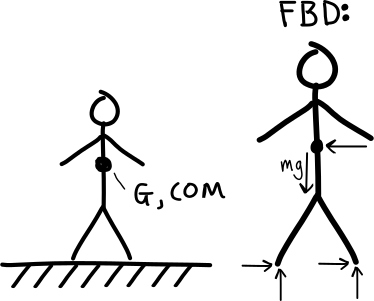
\includegraphics[width=0.4\textwidth]{Figures/PersonFBD}\par
\end{centering}
\caption[Diagram: Free Body Diagram of a Human]{Free body diagram of a human. For the point mass model of a human, the human is reduced to a single point mass located at its center of mass. The force of gravity acts at the center of mass, as well as air drag if it is included. The force of friction and the normal ground reaction act at the human's massless feet. Of course, internal forces do not appear in the free body diagram.\todo[inline]{Alan: I am not sure if that horizontal vector was meant to model drag or not when I drew this... I'm just hoping it wasn't for something that I'm forgetting right now. }}
\label{fig:PersonFBD}
\end{figure}
%

Although walking appears to be a smooth process, it can actually be viewed as a series of collisions. The collisional nature of this point mass motion is illustrated in figure \ref{fig:Bounce}. In essence, the point mass model of a human is a bouncing particle. The particle does not collide directly with the ground, but collides through massless legs. The objective here is to find a relation between the work $W$ performed by the locomotive and the metabolic energy cost $E_{m}$\index{metabolic cost} of providing that work \cite{ruina05}. This work is performed by the locomotive's muscles to overcome the collision of the point mass in each stride. Positive work denotes work done \emph{by} the muscles on the skeleton.

The stride, or gait cycle, is divided into a falling portion that occurs before the collision of the mass with the ground, and a rising portion after the collision. The collision provides an impulsive vertical upward force that results in a new vertical velocity of the mass. If drag is neglected, there are no forces in the horizontal direction and the locomotive travels at a constant horizontal speed.

The minus sign and positive sign in figure \ref{fig:Bounce} denote the motion before and after the collision. Before the collision, the leg muscles are in \emph{eccentric}\index{contraction!eccentric} contraction, which means they are elongating under tension. In this ``contraction'', the muscles are performing negative work on the body. After the collision, the leg muscles are in \emph{concentric}\index{contraction!concentric} contraction, which means they are shortening and doing positive work on the body.

% FIGURE
\begin{figure}[h]		% h="here" t="top" b="bottom" p="separate page"
\begin{centering}
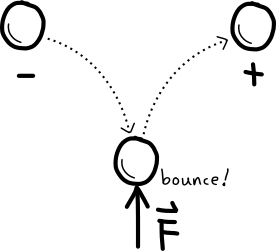
\includegraphics[width=0.3\textwidth]{Figures/Bounce}\par
\end{centering}
\caption[Diagram: Point Mass Model of Human Locomotion]{Point mass model of human locomotion. The human is a single point mass that periodically collides with the ground. The legs of the human are ignored so that the ground reaction is a single vertical force that helps redirect the velocity of the human. The minus sign and positive sign denote the motion before and after the collision.}
\label{fig:Bounce}
\end{figure}
%

Since we desire a relationship between energy (metabolic cost) and total work (muscle work) over a single stride, we apply the work-enegy theorem to this model over a single stride.

\begin{align}
P &= \vF \cdot \vv \notag \\
W &= \int \vF \cdot d\vr \notag \\
  &= E^{+}_{K} - E^{-}_{K} \notag \\
 &= \Delta E_K
\label{eq:CollisionalWork}
\end{align}
\index{collisional work}

where $E_{K}$ is the kinetic energy of the mass, $E_{K}^{+}$ is its kinetic energy after the collision, and $E_{K}^{-}$ is its kinetic energy before the collision. If we consider steady locomotion on level ground, then the motion is periodic and the kinetic energy does not change from stride to stride. By equation \ref{eq:CollisionalWork}, the net work from stride to stride must be zero as well. If the muscle work in a stride is divided into positive and negative portions as described above, then

\begin{equation}
W = W_{pos} + W_{neg} \approx 0
\label{eq:CollisionalWork2}
\end{equation}

equation \ref{eq:CollisionalWork2} is not an equality because some work goes into nonconservative energy dissipation, such as the deformation of parts of the body that are not muscle.

\todo[inline]{Alan: a general note on the use of "metabolic." The net-zero work concept makes sense if you're thinking only of work in the traditional energetics sense of the word. I feel like many people to whom this whole subject may be new would have trouble with the net-zero work concept because they may think "oh, well then why do I get tired, need to eat, etc. after walking with a steady periodic motion?" The answer is because the way muscles work, you still consume calories to do the negative work. It's not like we're getting energy back by falling. The next section explains this well, with the "b1" and "b2" constants, but the lead-in may be a little confusing. I don't know if this should be made explicit or not.}

We are now equipped to relate muscle work to metabolic energy cost. Recalling figure \ref{fig:MetabolicCost}, the metabolic cost can be expressed as

\begin{displaymath}
   E_{m} = \left\{
     \begin{array}{lr}
       b_{1} W & : W \geq 0\\
       b_{2} |W| & : W < 0
     \end{array}
   \right.
\end{displaymath}

where $E_{m}$ is always positive, $W$ is muscle work, $b_{1}$ is an empirical conversion factor for negative muscle work (as with the eccentric contraction), and $b_{2}$ is an empirical conversion factor for positive muscle work (as with the concentric contraction). The metabolic cost of one stride is then:

\begin{align}
E_{m} &= b_{1} W_{pos} + b_{2} |W_{neg}| \\
&\approx (b_{1} + b_{2})W_{pos}
\end{align}

Collecting in terms of $W_{pos}$ is possible because of the principles used to make the approximation in equation \ref{eq:CollisionalWork2}. If $W_{pos}$ is nearly equal to $|W_{neg}|$, one can be substituted for the other and the sum of the empirical constants $b = b_{1} + b_{2}$ may then be collected as one expression. Figure \ref{fig:MetabolicCost} indicates that $b_{1}\approx4$ and $b_{2}\approx1$. This means that the caloric energy spent by the body while walking is approximately 5 times the positive work required to move the body. 

\todo[inline]{[chris: can we quantify how much energy this actually is? I can use the discussion of muscles in section \ref{sec:IntroductionToMuscles}, or could refer the reader to employ methods provided in section \ref{sec:OptimizationInLocomotion}] \\ Alan: I think the best we can do is to refer people to section \ref{sec:OptimizationInLocomotion}. That deals with the integration along the path, which is really the only way to quantify the energy used (by the model).}

The trajectory traced by the center of mass in our point mass model shows that the motion is not smooth. This conflicts with our own perception of our motion as being a smooth process. The point mass motion is better applied to the motion of a hopping frog. This ``gait" is described by figure \ref{fig:HoppingFrogModel}. The definition for the cost of transport (COT) is easily applied here to provide 

\begin{equation}
COT = \frac{E_{m}}{mgd} = \frac{bW_{pos}}{mgd}
\end{equation}

For more detail about the hopping frog model, see Rashevsky 1948 \cite{rashevsky48}.

% FIGURE
\begin{figure}[h]		% h="here" t="top" b="bottom" p="separate page"
\begin{centering}
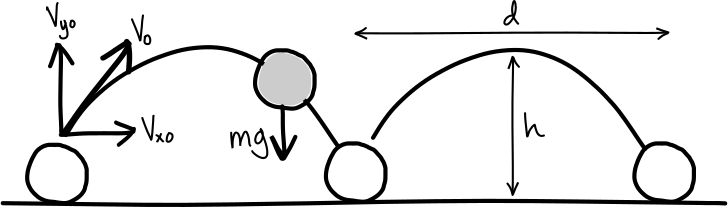
\includegraphics[width=0.8\textwidth]{Figures/HoppingFrogModel}\par
\end{centering}
\caption[Diagram: Hopping Frog Model]{Hopping frog model. The point mass model applies better to the motion of a hopping frog. This motion is characterized by two parameters: a jump distance $d$ and height $h$ of the hops.}
\label{fig:HoppingFrogModel}
\end{figure}
%

However, most animals continue traveling throughout this collision. In fact, the kinetic energy of a locomotive typically remains constant through steady motion \cite{ruina05}). Additionally, the up and down motion traced by the center of mass is usually much smaller than the forward motion. In terms of figure \ref{fig:HoppingFrogModel}, this means that the change in $h$ throughout a gait cycle is much smaller than $d$. For these reasons, we explore a more detailed model of the legs' trajectory and the forces upon the body from the ground.

\todo[inline]{Alan: the hopping frog model stuff either needs to be cut out, or explained better in a way that makes it clear why it's even here.}

\begin{comment}
For conservation of energy, the positive muscle work must be the same as the net mechanical energy lost in one stride \cite{ruina05}. 
\end{comment}

\section{The Collisional Model} % (notes page 12-19)
\label{sec:TheCollisionalModel}
\index{models of locomotion!collisional}

We developed the point mass model under the claim that legs can be ignored since the mass of legs is often significantly less than that of the whole body. However, legs are useful for accurately describing the collision of the body with the ground.

%[chris]: how do we deal with one leg at a time?

This model incorporates, initially, a single massless leg to allow for a more detailed force interaction \cite{ruina05}. A simple illustration of the collisional model is given in figure \ref{fig:LegDiagram}. The collision does not occur at a single point but over a contact region $W$ in between the falling and rising portions of the stride. Instead of a directly upward force upon the point mass from the ground collision, the force on the point mass is conveyed through the locomotive's legs throughout the entire contact region. The leg only conveys a force in compression, and there are no moments generated by the collision (e.g. a hip torque). Although the collision occurs over a distance, the collision still occurs quickly ($\Delta t \rightarrow 0$). As a result, the force associated with the impact dominates non-collision forces such as weight.

% FIGURE
\begin{figure}[h]		% h="here" t="top" b="bottom" p="separate page"
\begin{centering}
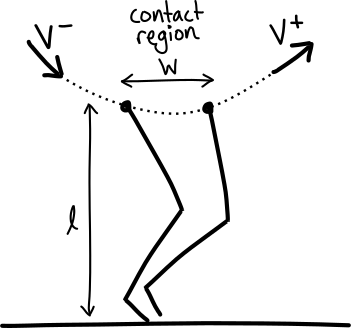
\includegraphics[width=0.4\textwidth]{Figures/LegDiagram}\par
\end{centering}
\caption[Diagram: Legs in the Collisional Model]{Legs in the collisional model. The impact of the ground on the locomotive is conveyed through massless legs. The impact occurs over a contact region $w$, which is the horizontal distance that the locomotive moves while (one of) its legs are in contact with the ground. The speed before the contact is $v^{-}$ and the speed after the collision is $v^{+}$. During the contact, the distance between the center of mass of the locomotive and the ground is approximated as $l$.}
\label{fig:LegDiagram}
\end{figure}
%

If we approximate that $W \ll l$, then the angle of the force $F$ is constant throughout the collision. In figure \ref{fig:CollisionDiagram}, the angle of the force is given by the unit vector $\hat{\lambda}$. The velocity of the point mass before and after the collision is given by $\mathbf{v}^{-}$ and $\mathbf{v}^{+}$, respectively. The collision causes a net deflection $\phi \ll 1$, which can be decomposed into components

\begin{equation}
\phi = \phi^{-} + \phi^{+}
\label{eq:PhiDecompose}
\end{equation}

that describe the direction of the initial and final velocities relative to the line given by $\hat{t}$.

%[chris]: is the rest of the mass, from waist up, considered to be a point mass?

% FIGURE
\begin{figure}[h]		% h="here" t="top" b="bottom" p="separate page"
\begin{centering}
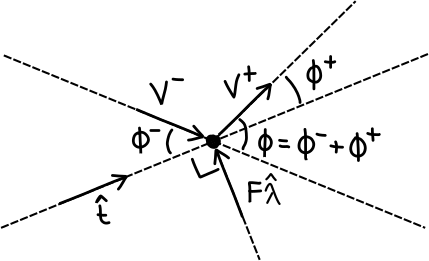
\includegraphics[width=0.5\textwidth]{Figures/CollisionDiagram}\par
\end{centering}
\caption[Diagram: Collisional Model Impulse]{Collisional model impulse. This diagram describes the change in velocity (direction and magnitude) that occurs during the collision of the leg with the ground. The contact $w$ is assumed to be small, but this diagram is ``located'' at the center of mass throughout the collision. The direction is constant in the direction of $\ul$. The unit vector $\ut$ is defined as perpendicular to $\ul$. The incoming deflection of the velocity is the angle $\phi^{-}$ between $v^{-}$ and $\ut$. The outgoing deflection of the velocity is the angle $\phi^{+}$ between $v^{+}$ and $\ut$.}
\label{fig:CollisionDiagram}
\end{figure}
%

\subsubsection*{Kinetic energy and the collision}

Collisions are classically viewed as dissipative interactions. In this case however, the muscular mechanisms involved in the collisions can even permit the interaction to increase the kinetic energy of the locomotive. We decompose the velocity of the point mass into components as $\mathbf{v} = v_{\lambda} \ul + v_{t} \hat{\mathbf{t}}$ so that we can write the kinetic energy of the mass as in equations \ref{eq:CollisionsKE}.

\begin{equation}
E_{K} = E = \frac{1}{2}m(v_{\lambda}^{2} + v_{t}^{2})
\label{eq:CollisionsKE}
\end{equation}

In this section, the kinetic energy is written as $E$ for clarity. The change in kinetic energy as a result of the collision is then $\Delta E = E^{+} - E^{-}$, where

\begin{align}
E^{-} &= \frac{1}{2}m[(v_{\lambda}^{-})^2 + (v_{t}^{-})^2]  \notag \\   
E^{+} &= \frac{1}{2}m[(v_{\lambda}^{+})^2 + (v_{t}^{+})^2] \notag
\end{align}

We can simplify these energy terms using the assumptions we have made. During the collision, no forces act in the $\hat{t}$ direction, so $v_{t}^{+} = v_{t}^{-}$. Since $\phi$ is small, $\sin{\phi} \approx \phi$ and so the velocity in the direction of $\hat{\lambda}$ before and after the collision is simply $v_{\lambda}^{-} = -v \phi^{-}$ and $v_{\lambda}^{+} = v \phi^{+}$.

% FIGURE
\begin{figure}[h]		% h="here" t="top" b="bottom" p="separate page"
\begin{centering}
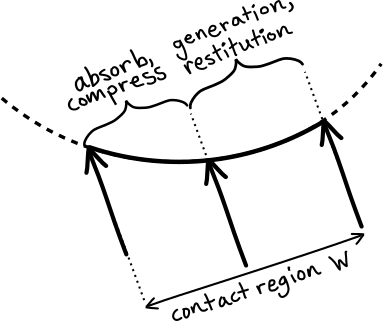
\includegraphics[width=0.4\textwidth]{Figures/BounceEnergy}\par
\end{centering}
\caption[Diagram: Energy in the Collisional Model]{Energy in the collisional model. The collision is divided into two portions: In the initial absorption portion, kinetic energy $E_{a}$ is absorbed (not all lost though) while the human approaches the ground. In the subsequent generation portion, the human generates and recovers kinetic energy in the quantity $E_{g}$ while starting to rise.}
\label{fig:BounceEnergy}
\end{figure}
%

The collision can be divided into two portions as in figure \ref{fig:BounceEnergy}, an absorption/compression portion and a generation/restitution portion, The change in kinetic energy across the collision can be written in terms of these portions of the collisions.

\begin{align}
\Delta E^{*} &= E_{g} - E_{a} \notag \\
  &= \frac{1}{2} m v^{2} \displaystyle\left[ (\phi^{+})^{2} - (\phi^{-})^{2} \displaystyle\right] \notag \\
 &= mv^{2} \left( \frac{\phi^2}{2} - \phi \phi^{-} \right)
\label{eq:GenerateAbsorbKE}
\end{align}

where $E_{a}$ is the absorbed energy and $E_{g}$ is the generated energy in the collision, the $v_{t}$ terms drop out, and equation \ref{eq:GenerateAbsorbKE} has made use of equation \ref{eq:PhiDecompose}. It is important to understand that this is the change in kinetic energy over just the collision, not over the entire gait cycle. For this reason, the change in kinetic energy is designated with a superscript asterisk. This distinction will be important when expressing the metabolic cost of locomotion later in this section. equation \ref{eq:GenerateAbsorbKE} has been written in its apparently contrived form to bridge it to an expression that employs impulse.

% FIGURE
\begin{figure}[h]		% h="here" t="top" b="bottom" p="separate page"
\begin{centering}
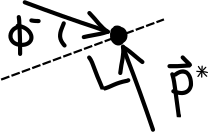
\includegraphics[width=0.18\textwidth]{Figures/Impulse}\par
\end{centering}
\caption[Diagram: Impulse in the Collisional Model]{Impulse in the collisional model. The impulse acts along the direction of the impact force $\ul$.}
\label{fig:Impulse}
\end{figure}
%

The impulse delivered to the point mass is $\mathbf{P}^{*} = P^{*}\hat{\lambda}$, as shown in figure \ref{fig:Impulse}. Using our approximations for velocity, the impulse is

\begin{align}
\vec{\mathbf{P}}^* &= mv(\phi^{+} - (-\phi^{-}))\ul\\
P^* &= mv\phi
\label{eq:CollisionImpulse}
\end{align}

Using this impulse, the two terms in equation \ref{eq:GenerateAbsorbKE} become

\begin{equation}
\Delta E^{*} = \frac{ (P^{*})^{2}}{2m} + \vec{\mathbf{P}}^{*} \cdot \vec{\mathbf{v}}^{-}
\label{eq:GAKE2}
\end{equation}

Equation \ref{eq:GAKE2} can be most easily understood by expressing its second term as equation \ref{eq:GenerateAbsorbIntermediate2} to arrive back at equation \ref{eq:GenerateAbsorbKE}.

\begin{align}
\vec{\mathbf{v}}^{-} &= v(-\phi^{-} \ul + 1\hat{\mathbf{t}}) \label{eq:GenerateAbsorbIntermediate1} \\
(P^{*} \ul) \cdot \vec{\mathbf{v}}^{-} &= (mv\phi)(-v\phi^{-})(\ul \cdot \ul) \label{eq:GenerateAbsorbIntermediate2}
\end{align}

where the small angle approximation $\cos{\phi} \approx 1$ has been made. In general, $\Delta E^{*}$ can be either positive or negative. \todo[inline]{chris: we don't use this form of delta E, so should we include it?}

Typically, the change in velocity of colliding masses is described by a \textit{coefficient of restitution} $e_{r}$, which is the relative speed of separation divided by the relative speed of approach of two colliding masses. This quantity is useful because it describes how elastic a collision is.

\begin{displaymath}
   e_{r} = \left\{
     \begin{array}{lr}
       1 & : \mbox{perfectly elastic}\\
       0 & : \mbox{perfectly plastic}
     \end{array}
   \right.
\end{displaymath}

For the collisional model, this coefficient is 
\begin{displaymath}
e_{r} = \frac{|v_{\lambda}^{+}|}{|v_{\lambda}^{-}|} = \frac{\phi^{+}}{\phi^{-}}
\end{displaymath}

However, this coefficient is not so useful for the scenario in which $\phi^{-} = 0$. This would be a ``collision'' that is not elastic, but actually ``generative'', such as jumping. Remember, the collision here is not necessarily strictly dissipative. For this reason we define a \textit{coefficient of generation} $e_{g}$. \index{coefficient of generation} \index{generation!coefficient of}

\begin{align}
e_{g} &= \frac{\mbox{[relative speed of separation] - [relative speed of approach]}}{\mbox{[relative speed of separation] + [relative speed of approach]}} \notag \\
&= \frac{\phi^{+} - \phi^{-}}{\phi^{+} + \phi^{-}}
\label{eq:CoefficientOfGeneration}
\end{align}

This cofficient has the properties:

\begin{displaymath}
   e_{g} = \left\{
     \begin{array}{ll}
     	1 & : \mbox{solely generative}, e_{r} = \infty\\
        0 & : \mbox{perfectly elastic}, e_{r} = 1\\
       -1 & : \mbox{perfectly plastic}, e_{r} = 0\\
     \end{array}
   \right.
\end{displaymath}

With some algebra,  $e_{g}$ for the collisional model can be expressed as 

\begin{displaymath}
e_{g}=\frac{\Delta E^{*}}{mv^{2}\phi^{2}/2}
\end{displaymath}

This is the ratio of the energy gained in the collision to the amount of energy that \emph{would} be in absorbed in a fully plastic collision with the same $v$ and $\phi$ \cite{ruina05}. This also yields another formula for the change in kinetic energy across the collision

\begin{equation}
\Delta E^{*} = e_{g} \frac{mv^{2} \phi^{2}}{2}
\label{eq:GenerateAbsorbKE3}
\end{equation}

We now endeavor to find the metabolic cost of locomotion for this collisional model, where the metabolic cost $E_{m} = b[\mbox{positive muscle work}]$. The quantity $b$ resembles an inverse efficiency, akin to a coefficient of performance from thermodynamics, and takes on a value between 4 and 5 for muscles and between 1.2 to 2 for motors. The \textit{elastic recovery coefficient} \index{elastic recovery coefficient} \index{coefficient!elastic recovery} $r$ is the fraction of absorbed energy $E_{a}$ that has been usefully or elastically stored and is thus available for muscle work as $E_{g}$, and $1-r$ is the fraction of absorbed energy that has been lost. This coefficient allows us to write

\begin{align}
\mbox{Positive generated muscle work} &= E_{g} - rE_{a} \\
\mbox{Absorbed energy that is lost} &= E_{a}(1-r)
\label{eq:ElasticRecovery}
\end{align}

The absorbed energy can be lost by general dissipation, or by negative muscle work that is not stored elastically.

\subsubsection*{Metabolic cost}

We now seek to determine the metabolic cost of locomotion using the collisional model. The collision occurs during only a small portion of the gait cycle. In general, energy interactions must occur during the other portions of the gait to maintain conservation of energy. Thus, the metabolic cost here is an \textit{inferred} metabolic cost \index{metabolic cost!inferred} because we assume that the minimum amount of positive work is performed throughout the remainder of the gait cycle. That is, the amount of positive work performed is only as much positive work as is required to recover from dissipation or energy loss in the collision. Basically, the locomotive is not kicking its feet between collisions.

We can express the metabolic cost in terms of $E_{a}$, $E_{g}$, and $r$. The use of an \textit{inferred} cost requires the examination of two different cases.

\begin{itemize}
\item \textbf{Dissipative collision}: $e_{g} \leq 0$, $\Delta E^* \leq 0$, $E_{g} \leq E_{a}$. Energy is lost over the course of the collision. To conserve energy, at least $E_a - rE_a$ positive work must be performed during the gait (outside of the collision). By using this quantity as the minimum positive work performed,

\begin{align}
E_{m}& = bE_{a}(1-r) \notag \\
 &= b\left(\frac{m v^{2} \phi^{2}}{8}\right)(1-r)(1-e_{g})^2
\label{eq:MetabolicCostCollisionalNeg}
\end{align}

For a perfectly plastic collision, $e_g$ = -1, with no energy recovery from muscles, $r$ = 0, $E_{m} = b E_{a}$.

\item \textbf{Generative collision}: $e_{g} \geq 0$, $\Delta E^* \geq 0$, $E_{g} \geq E_{a}$. Energy is gained over the course of the collision. Thus, the positive work performed throughout the gait must be at least the positive work performed during the collision.

\begin{align}
E_{m} &= b(E_{g} - r E_{a}) \notag \\
 &= b\left(\frac{m v^{2} \phi^{2}}{8}\right)\left[(1-r)(1-e_{g})^2 + 4e_{g}\right]
\label{eq:MetabolicCostCollisionalPos}
\end{align}

For a solely generative collision or jump from rest, $e_{g}$ = 1, with no energy recovery, $E_{m} = b \phi^2 v^2 m / 2$.
\end{itemize}

Again, the first case corresponds to a net energy loss during the collision, and a net energy gain during the remainder of the gait. The second case corresponds to a net energy gain during the collision, but a net energy loss during the remainder of the gait. In this formulation, it is assumed that the kinematic parameters $v$ and $\phi$ are known. The coefficients $e_{g}$ and $r$ could be obtained experimentally. The derivation of equations \ref{eq:MetabolicCostCollisionalNeg} and \ref{eq:MetabolicCostCollisionalPos} is left to the reader. A valuable result from these formulas is that a pseudo-elastic \index{pseudo-elastic} collision has a quarter of the metabolic cost of a fully plastic (absorbing) collision. A pseudo-elastic collision is just like a perfectly elastic collision in that the kinetic energy before and after the collision is the same (alas, $e_{g} = 0$) except that some energy $is$ dissipated in the collision but is replaced by additional muscle work. However, this is not apparent from the kinematics.

\subsubsection*{No-cost locomotion and multiple collisions}

Is it possible to achieve locomotion at no energy cost? \todo[inline]{chris: include why this would be neat} Logically, it is valuable to explore ways for a locomotive to minimize its $COT$. Remember that we have assumed that the cost of locomotion mostly comes from collisions. Then a model of locomotion in which collisions do not occur could potentially exhibit a very low $COT$. This question can be explored by examining \textit{brachiation}\index{brachiation}, which is the motion of swinging between overhead supports. This motion is exhibited by gibbon apes and by children on monkey bars. The kinematics of this motion is described in figure \ref{fig:Brachiation}. The locomotive's path alternates between pendular when swinging on a tree branch, and parabolic when in free flight subject to gravity \cite{bertram99}.

% FIGURE
\begin{figure}[h]		% h="here" t="top" b="bottom" p="separate page"
\begin{centering}
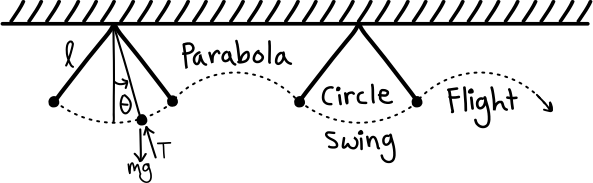
\includegraphics[width=0.7\textwidth]{Figures/Brachiation}\par
\end{centering}
\caption[Diagram: Brachiation]{Brachiation. Brachiation is the motion of swinging between overhead supports, as apes oft do. The motion consists of pendular swinging and a free flight. If the path of the motion is smooth, there is no collision and the motion is conservative.}
\label{fig:Brachiation}
\end{figure}
%
If the intersection of the parabola and circular arc is smooth (the direction of velocity is continuous), then no collision is required to redirect the locomotive's velocity from down to up. If no collision occurs, then the locomotion has no energy cost (neglecting friction). This model can be adapted to locomotion on the ground, since the model is analagous to upside-down running \cite{ruina05}. This can be done if the tension in the pendular motion is replaced with compression.

% FIGURE
\begin{figure}[h]		% h="here" t="top" b="bottom" p="separate page"
\begin{centering}
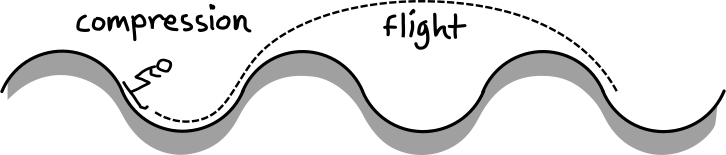
\includegraphics[width=0.7\textwidth]{Figures/Moguls}\par
\end{centering}
\caption[Diagram: Ski Slope Moguls]{Ski slope moguls. An analogue to brachiation is skiing on moguls, or small snow hills. The motion consists of a smooth path that alternates between ``compression'' and free flight.}
\label{fig:Moguls}
\end{figure}
%

A situation in which the pendular motion is characterized by compression is with skiing across snow moguls, as in figure \ref{fig:Moguls}. While in the trough between moguls, a skiier's velocity is redirected by a centripetal ``compressive" normal force. The skiier leaves the trough with a velocity that is parallel to the slope of the mogul at the point of departure. If the skiier enters the next trough with a velocity parallel to the mogul at the point of contact, then the velocity is continuous and no collision has occurred. In other words, no collision plane can be defined.

However, we have only moved the brachiation to the ground, and skiing is still very different from walking. A modified collisional model can resemble brachiation. In this modified collisional model, the locomotive experiences multiple collisions with the ground contact in each gait cycle rather than a single collision.

% FIGURE
\begin{figure}[h]		% h="here" t="top" b="bottom" p="separate page"
\begin{centering}
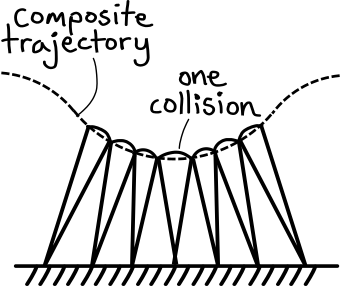
\includegraphics[width=0.3\textwidth]{Figures/MultipleCollisions}\par
\end{centering}
\caption[Diagram: Multiple collisions in the Collisional Model]{Multiple collisions in the collisional model. The collisional model is modified so that there are $n$ collisions per step, each conceivably executed by a different leg. The cost of locomotion is reduced by a factor of $n$ as compared to that for a one-legged locomotive.}
\label{fig:MultipleCollisions}
\end{figure}
%
\todo[inline]{chris: i think this entire chapter needs to be much clearer about what we're modeling. is it humans or what?}

Consider $n$ collisions that deflect the velocity of the locomotive by $\phi/n$, where $\phi$ is the total deflection from the $n$ collisions that is equivalent to the deflection $\phi$ from the single-collision model (figure \ref{fig:MultipleCollisions}). In this figure, it can be assumed that these $n$ collisions are executed by an $n$-legged locomotive and that each collision is performed by a different leg; the model is an abstraction from real scenarios. The parameters $v$, $e_{g}$ and $r$ are not changed in the $n$-collision model. Since the change in energy $\Delta E^*$ from a single collision is proportional to $\phi^2$, the metabolic cost for a single collision is reduced by a factor of $n^2$. Since these lower-cost collisions occur $n$ times, the \emph{total} cost of locomotion is reduced by a factor of $1/n$. As $n \rightarrow \infty$, the metabolic cost goes to zero.

This generalization allows the consideration of a number of gaits that describe at least two legs in the gait cycle. \todo[inline]{chris: gaits are discussed fundamentally in Optimization of Locomotion - Choosing a gait. should that be moved here? Alan: I think the section you're referring to is appropriate where it is, because it's discussing the choice in the context of optimization.} Four biped (two-legged) gaits are considered, as labeled (1) through (4) in the \textit{hodograph}\index{hodograph} in figure \ref{fig:Hodograph}. The hodograph contains plots of the velocity vector of the point mass as it evolves over the course of the collision. The full vector is only drawn in its initial and final positions, but the vector traces the dotted line path for the gait considered. The vector is plotted as always starting from the same location to depict how its magnitude changes as its direction changes by the full deflection $\phi$. The locomotive is indeed moving forward through the collision, though this is not apparent in the figure. The first of the two collisions is performed by a leg from a previous stance, and the second collision by a leg entering a new stance. Remember that velocity corresponds to a certain amount of kinetic energy, and for steady periodic motion the kinetic energy at the start of each gait cycle must be the same. Thus, the length of $v^{-}$ must be the same in every gait cycle. If negligible work is done during other portions of the gait, then the length of $v^{+}$ must be the same as the length of $v^{-}$. 

% FIGURE
\begin{figure}[h]		% h="here" t="top" b="bottom" p="separate page"
\begin{centering}
\subfloat[hodograph]{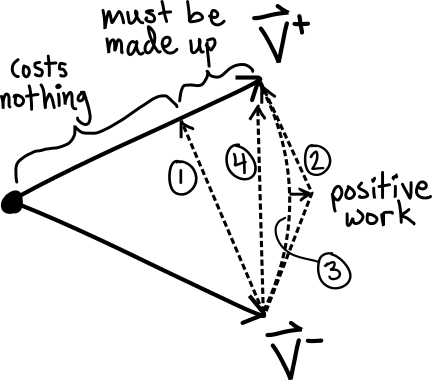
\includegraphics[width=0.3\textwidth]{Figures/Hodograph}\label{fig:Hodograph}}
\subfloat[incoming and outgoing impulses]{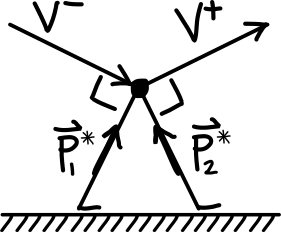
\includegraphics[width=0.3\textwidth]{Figures/StepTransition}\label{fig:StepTransition}}
\subfloat[simultaneous impulse force time history (for case 4)]{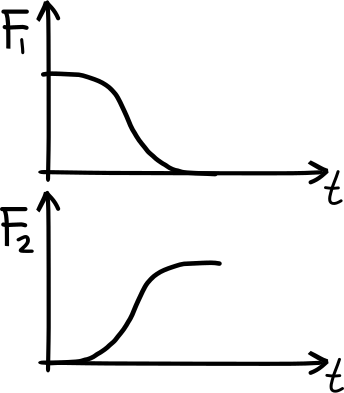
\includegraphics[width=0.3\textwidth]{Figures/ForcesFollowCircle}\label{fig:ForcesFollowCircle}}
\end{centering}
\caption[Diagram and Figure: Two-Collision Gaits in the Collisional Model]{Two-collision gaits in the collisional model. The hodograph (a) describes the four two-collision gaits explored in this section. A hodograph describes how a vector changes in both magnitude and direction by plotting the vector from the same point. The next diagram (b) shows the two impulses that belong to the first and second collisions that appear in some of the four gaits: the first impulse is perpendicular to the incoming velocity, and the second impulse is perpendicular to the outgoing velocity. The plots in (c) describe for case 4 the time history of the simultaneous forces that correpsond to the incoming and outgoing impulses. \todo[inline]{chris: subfigure captions need formatting}}
\label{fig:Ncollisional}
\end{figure}
%

\begin{itemize}
\item \textbf{Case 1, Fully plastic:} If the first impulse (collision) in figure \ref{fig:StepTransition} is taken away, then only the second impulse remains. This second instantaneous impulse removes the velocity along the direction of impact, and so this collision is purely plastic. The collision is termed ``passive" because no msucle work is performed during the collision. It is for this reason that this is the only case in which $v_{+}$ is not the same length of $v_{-}$. This means that the energy represented by the distance between the end of path (1) and the end of path (4) must be generated by work outside of the collision part of the gait cycle. The collision itself has an inferred metabolic cost $E_{m1} = \phi^{2} v^{2} m b/2$.

\item \textbf{Case 2, Pure generative-Pure absorbing:} As in figure \ref{fig:StepTransition} the first instantaneous impulse is purely generative, with $\phi^{-} = 0$ and $e_{g} = 1$. The second impulse is purely plastic/absorbing, as $\phi^{+} = 0$ and $e_{g} = -1$. The first impulse is a pre-emptive push-off from the previous stance. The second instantaneous impulse is part of the new stance.  If the first impulse is included, then the the inferred metabolic cost $E_{m2} = E_{m1}/4$ (using equation \ref{eq:MetabolicCostCollisionalPos}).

\item \textbf{Case 3, Constant energy:} The impulse to the point mass is always perpendicular to the velocity, and so no work is performed on the point mass. In the previous two cases, the impulses acted at different instantaneous times. In this case, however, both impulses act simultaneously over a short duration  of time as in figure \ref{fig:ForcesFollowCircle}. For this reason, the dotted path (3) in figure \ref{fig:Hodograph} is curved rather than piecewise linear as for the other cases. $F_{1}$ is the force corresponding to impulse $P_1^*$ and $F_{2}$ is the force corresponding to impulse $P_2^*$. The magnitudes of the forces vary so that the net impulse is always perpendicular to the velocity at a given instant. The inferred metabolic cost is $E_{m3} = E_{m1}/3$.

\item \textbf{Case 4, Simultaneous impulse:} The impulse is directly upward for the duration of the collision. This requires that $F_{1} = F_{2}$ throughout the collision. For this reason, the dotted path (4) is vertical. This has an inferred metabolic cost $E_{m4} = E_{m1}/2$.
\end{itemize}

This collisional model is fairly flexible, and can also be used to examine quadruped gaits, as with horses.

\todo[inline]{chris: this comes off as a theoretical ploy or an indication of an inconsistent theory; how can people actually walk so they're making multiple collisions? should make statement about how this is a mechanics theory. this section could also include a derivaiton of all inferred metabolic cost results for the 4 cases}

\section{Introduction to the SLIP Model} %(notes page 26)
\label{sec:SLIP}
\index{models of locomotion!SLIP}

The last three decades have seen substantial focus on a mass-spring model of locomotion that is now popularly called the Spring-Loaded Inverted Pendulum model. The model has prevailed because it is very simple but is rich in its ability to understand the control of locomotion. \todo[inline]{chris: i made this up, but i feel like it's true} For this reason, the model is explored in depth in sections \ref{sec:SpringLoadedInvertedPendulum} and \ref{sec:RaibertHoppingRobot}. For even more detail on the SLIP model, refer to Raibert \cite{raibert95}, Poulakakis \cite{poulakakis07,poulakakis07b}, and McGeer. The SLIP model is described by figure \ref{fig:SLIPSetup}. The locomotion is modeled with a single leg and a point mass body. The leg is a single massless link; there is no knee joint.

% FIGURE
\begin{figure}[h]		% h="here" t="top" b="bottom" p="separate page"
\begin{centering}
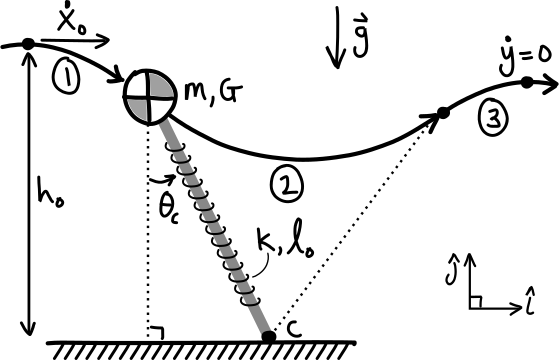
\includegraphics[width=0.7\textwidth]{Figures/SLIPSetup}\par
\end{centering}
\caption[Diagram: SLIP Model]{SLIP model. A point mass with mass $m$ at point $G$ is attached to a spring leg with spring constant $k$ and rest length $l_{0}$.  The gait starts when the position (x,y) of $G$  reaches the condition $\dot{y} = 0$. The subsequent motion is determined by the values for $\dot{x}_{0}$ and $h_{0}$. The leg makes contact with the ground at point $C$, and at contact is deflected from the vertical by an angle $\theta{c}$.}
\label{fig:SLIPSetup}
\end{figure}
%

The model is concerned with the stance portion of the gait cycle, which is defined in figure \ref{fig:SLIPGait} as the portion of the gait during which the leg is contacting the ground.  The initial conditions for a gait cycle are $\dot{x}_{0}$, the horizontal velocity, and $h_{0}$, the height of the locomotive, at the start of the gait cycle. The gait cycle starts at the point or moment at which $\dot{y}(x,t) = \dot{y}_{0}(x) = 0$. The angle that the leg makes with a vertical at the time of contact is $\theta_c$. The initial contact angle $\theta_c$ is the most important parameter in this model. For now, assume that $\theta_c$ is reset to the same value at the start of each stance. Later, $\theta_c$ will be controlled in order to explore the stability of the model. Throughout the stance, point C does not slip.

% FIGURE
\begin{figure}[h]		% h="here" t="top" b="bottom" p="separate page"
\begin{centering}
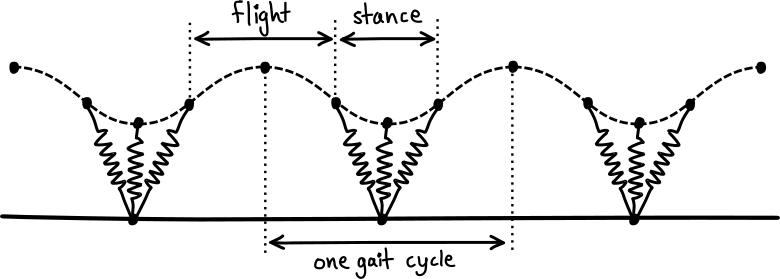
\includegraphics[width=0.9\textwidth]{Figures/SLIPGait}\par
\end{centering}
\caption[Diagram: SLIP Gait]{SLIP gait. The SLIP gait cycle can be divided into a flight, when the leg is not in contact with the ground, and a stance.}
\label{fig:SLIPGait}
\end{figure}
%

One way in which this model is distinct from the collisional model is that the contact of the locomotive with the ground is not impulsive. Additionally, it makes more sense to describe this model in terms of force interactions, rather than energy interactions as for the point mass and collisional models. The leg is modeled as a spring with spring constant $k$ and rest length $l_0$. As a result, the motion is also fully elastic, not quasi-elastic. This means that locomotion in this model is more efficient than in most cases of the collisional model since there is energy dissipation in the collisional model.

The gait cycle is divided into three portions, as denoted in figure \ref{fig:SLIPSetup}: (1) incoming flight, (2) stance, and (3) outgoing flight. The free body diagrams in figure \ref{fig:SLIPFBD} correspond to the three portions of the gait cycle. Linear momentum balance on the point mass yields

\begin{displaymath}
   m\vec{\mathbf{a}} = \left\{
     \begin{array}{ll}
        -mg \hat{\mathbf{j}} & : \mbox{flight, (1) and (3)} \\
       -mg \hat{\mathbf{j}} + \hat{\mathbf{F}}_s & : \mbox{stance, (2)} \\
     \end{array}
   \right.
\end{displaymath}

where $\hat{\mathbf{F}}_s$ is given by Hooke's Law,

\begin{equation}
\vec{\mathbf{F}}_s = k (l_0 - |\vec{\mathbf{r}}_{G/C}| ) \frac{\vec{\mathbf{r}}_{G/C}}{|\vec{\mathbf{r}}_{G/C}|}
\end{equation}

% FIGURE
\begin{figure}[h]		% h="here" t="top" b="bottom" p="separate page"
\begin{centering}
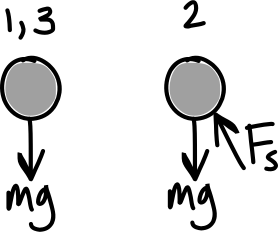
\includegraphics[width=0.2\textwidth]{Figures/SLIPFBD}\par
\end{centering}
\caption[Diagram: Free Body Diagrams for the SLIP Model]{Free body diagrams for the SLIP model. The locomotive in the SLIP model is a point mass. The left free body diagram corresponds to flight (labeled 1 and 3 in figure \ref{fig:SLIPSetup}) and the right free body diagram corresponds to stance. In stance, the force conveyed through the leg $F_{s}$ changes direction, unlike in the collisional model.}
\label{fig:SLIPFBD}
\end{figure}
%

The outgoing flight begins when the length of the leg returns to its rest length. During the flight, the locomotive follows a parabolic trajectory. This is similar the brachiation\index{brachiation} discussed in section \ref{sec:TheCollisionalModel}.

Although figure \ref{fig:SLIPGait} in this section seems to indicate that the SLIP motion is perfectly periodic, the motion over several gaits is not necessarily so. The motion is only periodic if $\dot{x}(t)$ and $h(t)$ take on the initial values $\dot{x}_{0}$ and $h_{0}$ at the end of the first gait cycle when $\dot{y}(t) = 0$. A periodic gait cycle means that the motion is stable. Logically, it is the stable case that is interesting, The stable motion is characterized by appropriate choices for $\dot{x}_0$ and $h_0$, depending on the other parameters of the model. The SLIP model can portray both walking and running depending on how $\dot{x}_0$ and $h_0$ are chosen. Both modes of locomotion can be stable.


[chris: if we want to talk about actual numbers for metabolic cost, see Ruina's simplest walker paper]



%%%%%%%%%%%%%%%%%%%%%%%%%%%%%%%%%%%%%%%%%%%%%%%%

\chapter{Passive Dynamics of Legged Locomotion}
\label{sec:PassiveDynamicsOfLeggedLocomotion}
\index{passive dynamics}

In section \ref{sec:SLIP} it was said that the SLIP locomotive could achieve
stable motion if initial conditions are appropriate. The fact that such motion
can sustain itself without any active feedback or input (an isolated system)
means the motion is passively stable. Thus, it may be possible to achieve
locomotion passively. This has various implications, especially for the design
of efficient (and thus more human-like) walking robots \cite{collins}. To build
up to an analysis of passive SLIP motion, we first examine the passive 2D
motion of a rimless wheel rolling down an incline.


%%%%%%%%%%%%%%%%%%%%%%%%%%%%%%%%%%%%%%%%%%%%%

% I just put this section here from the "introduction to stability" It may be spread around to other places. 

\section{Introduction to Stability} % (notes page 20-26)
\label{sec:IntroductionToStability}
\index{stability}

Understanding the passive dynamics of the models presented in Chapter
\ref{sec:ModelingLeggedLocomotion} requires a basic understanding of the
concept of stability. We consider locomotion to be a stable periodic motion of
a dynamic system, where the dynamic system is defined by ordinary differential
equations and sometimes collision equations. The motion of a dynamic system is
considered to be stable when the system is capable of rejecting disturbances.
A legged animal or robot that is moving with a stable gait, given some
perturbation in its motion, will return to the motion it was performing before
the perturbation was introduced. Experiment and theory have both shown that
certain legged animals and robots can walk or run with a stable motion without
any control; the motion is passively stable. We will see later on that the
mathematical description for such motion is a stable fixed point on a Poincare
section or map. 

% FIGURE
\begin{figure}[h]		% h="here" t="top" b="bottom" p="separate page"
\begin{centering}
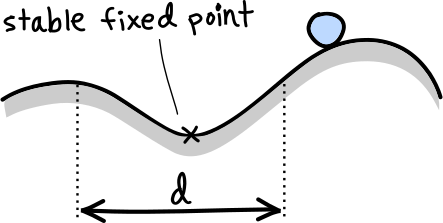
\includegraphics[width=0.55\textwidth]{Figures/BallOnHill}\par
\end{centering}
\caption[Diagram: Ball in a Valley]{Ball in a valley. If the ball is released
from the hill to the right at a height that is no greater than that of the hill
to the left, the ball will remain in the valley between hills. After some time,
the ball comes to rest at the stable fixed point at the bottom of the valley.
The steady state position of the ball can also be thought of as periodic motion
in which the ball is found at the stable fixed point at the end of each period
of the motion. This periodic motion mindset is useful for locomotion models.}
\label{fig:BallOnHill}
\end{figure}
%

Imagine a system like the one shown in figure \ref{fig:BallOnHill}: two hills,
with a valley between them, and a ball that starts on the side of the larger
hill. Imagine that the interaction between the ball and the hill is \emph{not}
frictionless, but the rolling resistance is small. When the ball is released,
it rolls left down the hill, passing by the lowest point in the valley,
and rolls over the peak of the smaller hill. Now imagine the ball starts a
little bit lower on the side of the larger hill, such that it rolls through the
valley, and does not roll past the peak of the smaller hill. It reaches some
maximum height, and rolls back the way it came. The ball oscillates back and
forth until it comes to rest at the bottom of the valley. 

Though slightly un-intuitive, one can think of the motion of the ball as
periodic in time. When the ball is resting at the bottom, we consider the ball
to be in ``motion," where the period of the motion is infinitesimal. The
resting point is considered a stable fixed point, because for every period of
the motion, the ball returns to that point. If the ball's ``motion" is
disturbed by an external force, after some number of periods it will return to
the stable fixed point. In this case, it is a little silly to think of it that
way, because between periods, the ball is still at stable fixed point during
its ``motion." \todo{get rid of preceding sentence?} The path that it
follows along the hill as it settles to that fixed point can be thought of as
the basin of attraction: if the ball starts anywhere in the basin, it reaches
the stable fixed point. 

In the case of the ball in figure \ref{fig:BallOnHill}, the basin of attraction
is two-dimensional. The ball can be assumed to be on the surface of the hill,
and its state can be described by two parameters: position along the path, and
velocity in the direction of travel. A Poincare map is a visualization of these
two parameters sampled once per period, in two-dimensional space, as in figure
\ref{fig:BasinOfAttraction}. Parameters like position and velocity can be
assigned to the $x$ and $y$ axes of the Poincare map, and the stable fixed
point can be located on the map. Figure \ref{fig:BasinOfAttraction} is a
generalized version of a Poincare map. In the case of the ball on the hill, the
stable fixed point would be at position $y = 0$ and velocity $x = 0$. A general
fixed point is marked with a star on the map, as shown in figure \ref{fig:BasinOfAttraction}. 

% FIGURE
\begin{figure}[h]		% h="here" t="top" b="bottom" p="separate page"
\begin{centering}
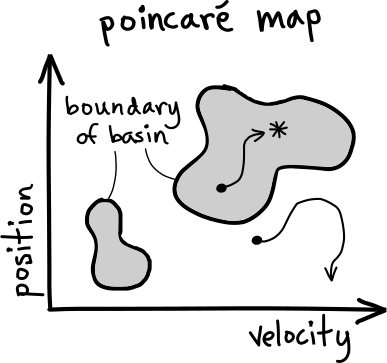
\includegraphics[width=0.3\textwidth]{Figures/BasinOfAttraction}\par
\end{centering}
\caption[Diagram: Poincare Map with Basins of Attraction]{Poincare map with basins of attraction. The map, drawn here for a general system, has coordinates of position and velocity. Points on the map denote the position and velocity state of a system at the end of each period of the system's motion. Basins of attraction are shaded, and fixed points are labeled as stars. If the initial state of a system, denoted as a dot, is within a basin of attraction, the system will tend toward the fixed point contained in that basin. If the initial state lies outside a basin, its configuration in time does not tend toward a particular steady motion.}
\label{fig:BasinOfAttraction}
\end{figure}
%

\todo{can there be a basin of attraction without a fixed point, as is
shown in the figure?}

The basin of attraction is made up of all the states (position and velocity)
that the system can have initially and still return to the stable fixed
point. In the ball example, it is important to note that the ball may start in
the region $d$ shown in figure \ref{fig:BallOnHill}, but if the velocity is
nonzero and too great, the ball may never reach the stable fixed point. 

\todo{change the previous sentence to ``if the velocity is
leftward, the ball will never reach the stable fixed point''?}

In general, it is possible to have part of the basin of attraction detached
form the part that contains the fixed point, as is shown in figure
\ref{fig:BasinOfAttraction}.

The stable fixed point is generally called an attractor, and up to this point
we have been thinking of the attractor as a single point on the Poincare map.
However, it is also possible that the attractor could be a complicated curve or
region. These complicated regions are sometimes called ``strange attractors."
Functionally, strange attractors are the same as a stable fixed point. If the
state of the system lies within the attractor, it will return to somewhere else
within that attractor one period later, just as a system would return to the
stable fixed point one period later. Figure \ref{fig:Attractors} shows the
difference between the two attractors.

% FIGURE
\begin{figure}[h]		% h="here" t="top" b="bottom" p="separate page"
\begin{centering}
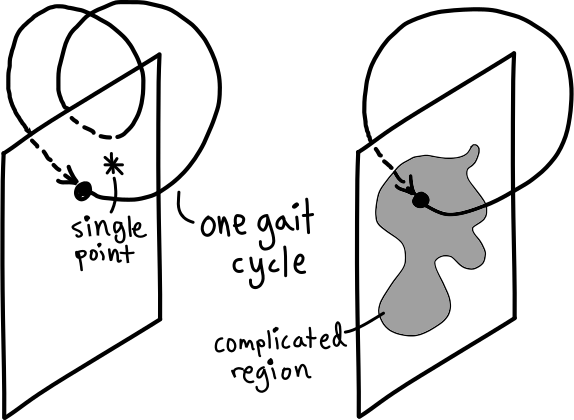
\includegraphics[width=0.5\textwidth]{Figures/Attractors}\par
\end{centering}
\caption[Diagram: Single Point Attractors and Strange Attractors]{Single point
attractors and strange attractors. The left Poincare section is for a single
point attractor, denoted by the star. The right Poincare section is for a
strange attractor, where the shaded area is the strange attractor. If the
system's state is within an attractor region, the system's state at the end of
each period will lie within the attractor. Note that the basin of attraction is
not shown for either attractor. The strange attractor on the right could be
enclosed by a larger basin of attraction. If a disturbance is introduced that
doesn't move the trajectory outside the basin of attraction, the trajectory
will return to the complicated region after some time.}
\label{fig:Attractors}
\end{figure}
%

\todo[inline]{I like how the loop shows a period. maybe axes again would help?
I don't know. Also this might be confusing since gray
was also used to show the basin of attraction in a previous figure. Also the
figure seems to indicate that for a strange attractor, for every period you do
come back to the same state.}

The section shown on the left of figure \ref{fig:Attractors} is an example of a
single point attractor, showing what might happen if a disturbance is
introduced. The trajectory traced around the section shows that the motions are
periodic, and do not quite pass through the stable fixed point on each period.
As long as the trajectory of the state passes through the basin of attraction,
the trajectory of the state will return to the stable fixed point, and become a
single loop like in the section shown on the right. 

As may be apparent from the previous two figures, much of our analysis of
stability is rooted in the state-space representation of systems. In such a
representation, there is a state at which the robot is operating. If we
introduce a disturbance to the state, perhaps $\epsilon$, we want to know if
the state space representation returns to what it was before the disturbance
was introduced. More tools for analyses like this can be found in books on
feedback control, such as Ogata \cite{ogata09} (Root Locus, Nyquist, etc).
These tools will not be used extensively in this chapter, but understanding the
reasons for their use in other systems will be helpful to understanding
stability analyses of legged locomotion models. 

%%%%%%%%%%%%%%%%%%%%%%%%%%%%%%%%%%%%%%%%%%%%

\section{Rimless Wheel} % (notes page 20-26)
\label{sec:RimlessWheel}
\index{rimless wheel dynamics}

The motion of a rimless wheel is a classical problem that exhibits some basic
aspects of passive stable motion and permits a nice introduction to examining
the stability of locomotion models. Consider the rimless wheel in figure
\ref{fig:RimlessWheel}, with massless spokes and a mass $m$ at its center, that
is rolling down an incline $\gamma$ under the force of gravity along $\ul$. The
wheel has $N$ spokes of length $l$, and each spoke is separated from the next
by the angle $\phi$. The moment of inertia of the wheel about its center $G$ is
$I$. The angle between the incline's normal and the spoke that is in contact
with the incline is $\theta = \theta(t)$. The wheel pivots without slip about
the end of this spoke, at point $C$. While pivoting, the wheel's center of mass
undergoes a motion that can be described as \textit{unstable falling}
\cite{coleman96}. This smooth motion occurs in between the plastic collisions
of the spokes with the incline.

% FIGURE
\begin{figure}[h]		% h="here" t="top" b="bottom" p="separate page"
\begin{centering}
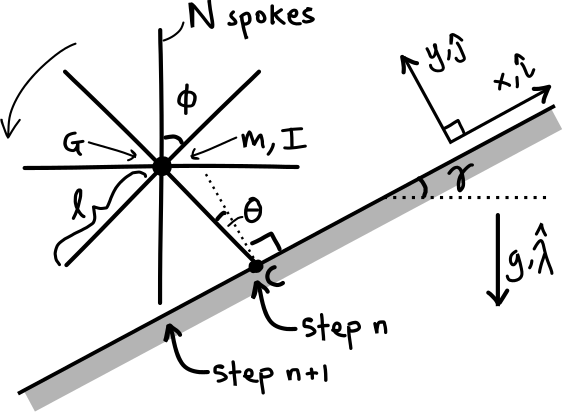
\includegraphics[width=0.6\textwidth]{Figures/RimlessWheel}\par
\end{centering}
\caption[Diagram: Rimless Wheel]{Rimless wheel. A rimless spoked wheel rotates
down an incline with slope $\gamma$. The $N$ massless spokes of length $l$ are
separated equally by the angle $\phi$ . The mass $m$ is located at the center of
the wheel, and the wheel has moment of inertia $I$. The orientation of the
wheel is specified by the angle $\theta$ that the spoke contacting the incline
makes with the incline's normal.}
\label{fig:RimlessWheel}
\end{figure}
%

Our objective with the rimless wheel is to compute its motion, given the
parameters above, and to examine its stability. The motion has two portions:
smooth motion and collisions.  The motion is most likely (but not necessarily)
periodic, so these two portions repeat again and again. Under the right
conditions, the wheel is able to achieve stable motion without any active
control.

\textbf{Smooth ``flight":} The velocity of the mass is continuous between
collisions. Angular momentum balance is a natural choice for finding the
motion, since angular momentum balance about point $C$ avoids the
undesired unknown of the reaction force at $C$. Using the free body diagram in
figure \ref{fig:RimlessSmoothAndCollision}a,

\begin{align}
\Sigma \vec{\mathbf{M}}_{/C} &= \dot{\vec{\mathbf{H}}}_{/C} \notag \\
l \hat{\mathbf{e}}_r \times mg \ul &= \vec{\mathbf{r}}_{G/C} \times m\vec{\mathbf{a}}_G + I \dot{\omega} \hat{\mathbf{k}}
\label{eq:RimlessAMB}
\end{align}

where $\hat{\mathbf{e}}_{r}$ is a unit vector pointing from the contact point $C$ to the center of mass of the wheel $G$. The unit vectors in equation \ref{eq:RimlessAMB} can be written explicitly, and the acceleration can be written in polar coordinates.

\begin{align}
\hat{\mathbf{e}}_{r} &= - \sin{\theta} \ui + \cos{\theta} \uj \\
\ul &=  - \sin{\gamma} \ui - \cos{\gamma} \uj \\
\va_{G} &= l \thetaddot \ueth - l \thetadot^{2} \uer
\end{align}

After substituting these expressions into equation \ref{eq:RimlessAMB}, employing the trigonometric sine sum identity and performing some additional algebra, we arrive at a system of two first-order nonlinear differential equations that can be solved perhaps with a computer solver.

\begin{align}
\dot{\theta} &= \omega \label{eq:RimlessODE2} \\
\dot{\omega} &= \frac{mgl}{I + m l^2} \sin(\theta + \gamma) \label{eq:RimlessODE1}
\end{align}

This equation of motion is very similar to that of an inverted pendulum,
considering that the coefficient in equation \ref{eq:RimlessODE1} is constant,
and that $\gamma$ is constant as well. As with any differential equation in
time, its solution requires initial conditions. The rotation of the wheel
initially is $\theta_{0} = \theta_n^{+}$, the rotation at the end of the $n$-th
collision. We choose this to be $-\phi/2$ because the end of the collision is
ambiguous. The angular speed at the start of the ``flight'' is $\omega_{0} =
\omega_{n}^{+}$, the angular speed of the wheel after the $n$-th collision. For
the first flight, this value is simply chosen. For subsequent motion, this
value comes from the spoke collision calculation for the $n$-th collision. To
obtain this, we must examine the spoke collision.

\textbf{Spoke collision:} Initial conditions for the angular speed \emph{after} the first ``flight'' are required to solve equations \ref{eq:RimlessODE2} and \ref{eq:RimlessODE1}. The initial position $\theta_{n+1,0}$ is always set as $\phi/2$, but the initial angular speed $\omega_{n+1,0}$ takes on the the angular speed at the end of the $n$+1-th collision, $\omega_{n+1}^{+}$. It is the objective of this spoke collision calculation to determine $\omega_{n+1}^{+}$ from the angular speed before the collision $\omega_{n+1}^{-}$. This relationship is found from conservation of angular momentum about point $C$ when the wheel is in the configuration shown in figure \ref{fig:RimlessSmoothAndCollision}b.

\begin{align}
\vec{\mathbf{H}}_{/C,n+1}^{-} &= \vec{\mathbf{H}}_{/C,n+1}^{+}
\label{eq:RimlessAM}
\end{align}

If there are no external torques about the point about which the angular momenum is calculated, then the angular momentum direclty before and directly after the collision must be the same. The only force that could cause a moment about the pivot point $C$ is the weight of the center of the wheel. However, the collision occurs over a short enough time period that the weight can be ignored. Again, the contact impulse at point $C$ does not contribute to the angular momentum about point $C$.

% FIGURE
\begin{figure}[h]		% h="here" t="top" b="bottom" p="separate page"
\begin{centering}
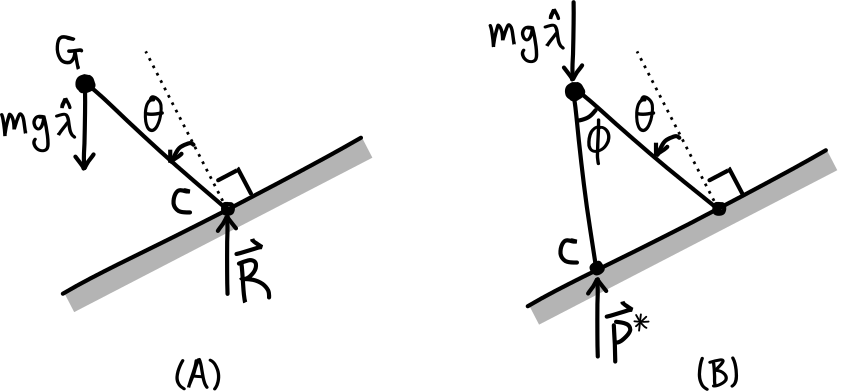
\includegraphics[width=0.7\textwidth]{Figures/RimlessSmoothAndCollision}\par
\end{centering}
\caption[Diagram: Rimless Wheel Free Body Diagrams]{Rimless wheel free body diagrams. Diagram (A) is a free body diagram for the smooth ``flight'' of the wheel. Diagram (B) is a free body diagram for the spoke collision of the wheel.}
\label{fig:RimlessSmoothAndCollision}
\end{figure}
%

The angular momentum before collision $n+1$ is

\begin{equation}
\vec{\mathbf{H}}_{/C,n+1}^{-} = \vec{\mathbf{r}}_{G/C} \times m\vec{\mathbf{v}}_{G}^{-} + I \omega_{n+1}^{-} \vec{\mathbf{k}}
\label{eq:RimlessHMinus}
\end{equation}

The angular momentum after collision $n+1$ is

\begin{equation}
\vec{\mathbf{H}}_{/C,n+1}^{+} = (I + ml^{2} ) \omega_{n+1}^{+} \hat{\mathbf{k}}
\label{eq:RimlessHPlus}
\end{equation}

Here, the moment of inertia used is about point $C$. Accordingly, this moment of inertia is the sum of the centroidal moment of inertia and a term from the parallel axis formula. By equating these two momenta and expressing explicity all the terms in equation \ref{eq:RimlessHMinus}, the angular speed after the collision is given by

\begin{equation}
\omega_{n+1}^{+} = \frac{I + ml^{2} \cos{\phi}}{I + ml^2} \omega_{n+1}^{-}
\label{eq:RimlessOmegaPlus}
\end{equation}

We see that the angular speed changes by a factor that depends only on the mass
and geometry of the wheel.

Now that we have our initial conditions for the smooth flight. we can piece
together the ``flight'' and collision. A qualitative description of the rimless
wheel motion is given by the graphs in figure \ref{fig:RimlessPlots}. Collision
$n$ ends at $t = 0$ and collision $n+1$ starts at $t = t^*$. The wheel rotates
quickly with $\omega = \omega_{n}^{+}$ right after the collision. Depending on
$\phi$, the mass may start its smooth ``flight'' motion before or \emph{at} the
apex of its ``flight'' path. If $\phi$ is sufficiently large, the mass slows
down as its mass is elevated to the apex of the path. If not, the mass starts
its ``flight'' at the apex.  The minimum angular speed is achieved at the apex
of the smooth "flight". The wheel accelerates downward from its apex as the
next spoke approaches collision. Just before the collision, the wheel rotates
with angular speed $\omega = \omega_{n+1}^{-}$ (figure
\ref{fig:RimlessPlots}b).

% FIGURE
\begin{figure}[h]		% h="here" t="top" b="bottom" p="separate page"
\begin{centering}
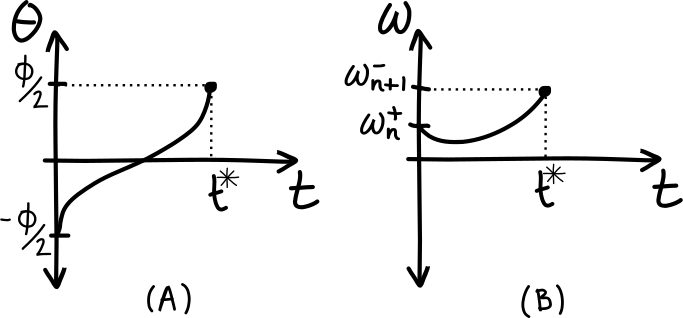
\includegraphics[width=0.7\textwidth]{Figures/RimlessPlots}\par
\end{centering}
\caption[Plot: Rimless Wheel State vs. Time for Smooth ``Flight'']{Rimless
wheel state vs. time for smooth flight. Plot (A) shows the rotation of the
wheel throughout the smooth ``flight'', up until the time $t^{*}$ when the
collision occurs. The flight is defined as occuring between $\theta = -\phi/2$
and $\theta = \phi/2$. Plot (B) shows the angular speed throughout the smooth
``flight'', which starts at $\omega_{n}^{+}$ and ends at $\omega_{n+1}^{-}$.}
\label{fig:RimlessPlots}
\end{figure}
%
\begin{comment}
 The dip in the curve depends on the the spoke separation $\phi$.
\end{comment}

% FIGURE
\begin{figure}[h]		% h="here" t="top" b="bottom" p="separate page"
\begin{centering}
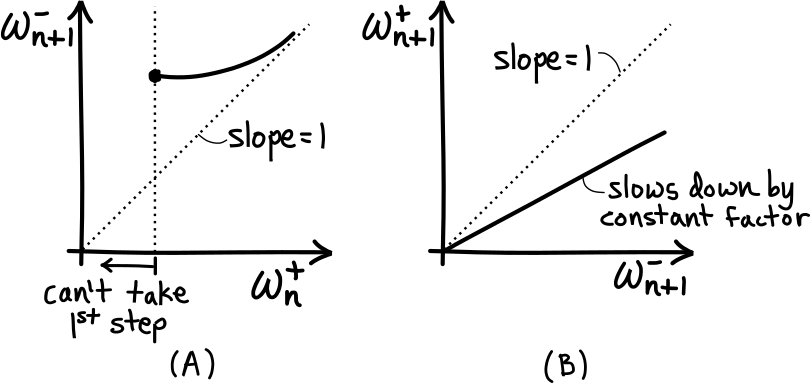
\includegraphics[width=0.7\textwidth]{Figures/RimlessPlots2}\par
\end{centering}
\caption[Plot: Rimless Wheel Angular Speed Relations]{Rimless wheel angular speed relations. Plot (A) provides $\omega_{n+1}^{-}$ at the end of the ``flight'' from $\omega_{n}^{+}$ from the beginning of the ``flight''. Plot (B) provides the angular speed after the collision $\omega_{n+1}^{+}$ from the angular speed before the collision $\omega_{n+1}^{-}$.}
\label{fig:RimlessPlots2}
\end{figure}
%
\begin{comment}
The curve asymptotically approaches $\omega_{n+1}^{-} = \omega_{n}^{+}$ as gravity has less time to accelerate the wheel for faster initial angular speeds. 
\end{comment}

The periodic evolution of the wheel's angular speed before and after collisions
is described by figure \ref{fig:RimlessPlots2}. Figure \ref{fig:RimlessPlots2}a
describes the change in angular speed between the beginning and end of the
smooth flight. There is a threshold value below which continued motion is not
possible and the wheel does not proceed continually down the incline. In this
case the wheel does not have enough momentum after the collision to move
through the apex of the smooth flight path. For greater initial speeds
$\omega_{n}^{+}$, the wheel starts the smooth flight with more momentum and
thus finishes the flight with a greater final speed $\omega_{n+1}^{-}$. The
curvature in this relation results from the fact that the force of gravity
contributes less to the increased final speed for higher values of the initial
speed. For large $\omega_{n}^{+}$ the flight occurs quickly enough that the
downward acceleration due to gravity does not have the time to noticably
increase the speed of the wheel.

Figure \ref{fig:RimlessPlots2}b picks up where figure \ref{fig:RimlessPlots2}a
leaves off, literally. This figure provides the difference between the speed
$\omega_{n+1}^{-}$ before the subsequent collision and the speed
$\omega_{n+1}^{+}$ after the subsequent collision.  \todo{The angular speed of
the wheel is discontinuous through the collision since the collision is not
elastic. chris: i now think the collision is elastic} The slope of the straight
line in figure \ref{fig:RimlessPlots2}b is given by the constant factor in
equation \ref{eq:RimlessHPlus}. The slope here can be thought of as a
coefficient of restitution.

\begin{comment}
Keep in mind that the curves in these plots are dependent on the parameters of
the rimless wheel model. For example, if $\gamma = 0$ then the incline becomes
a flat surface and the motion is not as interesting as for the general case
examined here. \todo[inline]{Chris: remove?: If $\gamma = 0$, the motion cannot
be stable if the collisions are not perfectly elastic.}
\end{comment}

% FIGURE
\begin{figure}[h]		% h="here" t="top" b="bottom" p="separate page"
\begin{centering}
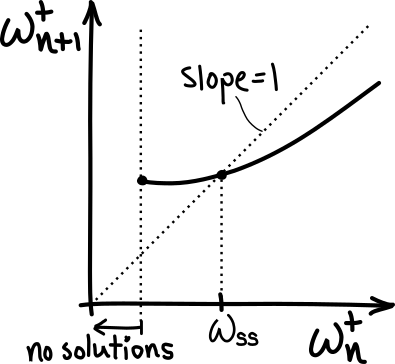
\includegraphics[width=0.3\textwidth]{Figures/RimlessStrideFunction}\par
\end{centering}
\caption[Plot: Rimless Wheel Stride Function]{Rimless wheel stride function. Provides the angular speed at the start of a ``flight'' from the angular speed at the start of the previous ``flight''. This figure is generated from a composition of the plots in figure \ref{fig:RimlessPlots2}. The point at which the curve intersects the $\omega_{n+1}^{+} = \omega_{n}^{+}$ line is a stable fixed point.}
\label{fig:RimlessStrideFunction}
\end{figure}
%

We now consider the stability of the rimless wheel. The composition of the
graphs in figure \ref{fig:RimlessPlots2} yields figure
\ref{fig:RimlessStrideFunction}, which is called a \emph{stride
function}\index{stride function}. The stride function can be used to understand
how the motion of the wheel evolves over numerous collisions. To determine the
motion of the wheel, or $\omega_{n+1}$, throughout multiple cycles of its
motion, use the following procedure with figure
\ref{fig:RimlessStrideFunction}:

\begin{enumerate}
\item Choose an initial value $\omega_{0}^{+}$ on the $\omega_{n}^{+}$-axis.
\item Trace this point up to the thick curve. This point on the thick curve provides the value of $\omega_{1}^{+}$ on the vertical axis.
\item Now $n = 1$; find the value of $\omega_{1}^{+}$ on the horizontal axis by
    tracing horizontally to the \textit{slope = 1} line.
\item Trace vertically from the \textit{slope = 1} line to the thick line to discover the value of $\omega_{2}^{+}$ on the vertical axis.
\item Repeat.
\end{enumerate}

\todo[inline]{Chris: I'd say we should put in a basin of attraction plot here
but am I right that we cannot do so, since, there is only one variable, that
determines stability?}

Again, the angular speed at the beginning of the smooth flight must surpass a
threshold value. If the initial angular speed in a given period has the steady
state value $\omega_{ss}$, then the subsequent motion is steady and periodic
until the wheel is perturbed. Note that the threshold angular speed, the steady
state angular speed, and the shape of the curve in the figure are all functions
of the model's parameters. Since the curve is increasing everywhere, all values
of $\omega_n^+$ above the threshold cause $\omega_n^+$ (and $\omega_{n+1}^{+}$)
to tend toward $\omega_{ss}$. That is, this system always tends toward the
stable fixed point $\omega_{ss}$ for the parameters used for figure
\ref{fig:RimlessStrideFunction}.

\section{Spring Loaded Inverted Pendulum} %(notes page 27-30)
\label{sec:SpringLoadedInvertedPendulum}

We now return to the SLIP model presented in section \ref{sec:SLIP} and analyze
its passive stability. In order to do so, we must first give careful thought to
the construction of its Poincare map.

Remember that the Poincare map is constructed by sampling the variables that
describe the motion of the system once per period, and plotting those points.
Therefore, we must assume that the model travels with a periodic gait. For the
SLIP model of walking and running, the system's state can be fully described by
four state variables related to the model's center of mass: $x$, $y$,
$\dot{x}$, and $\dot{y}$. The contact angle of the leg, $\theta_{c}$, is
considered to be an initial condition, and is not a part of the system state.

The point at which one ``slices'' the gait cycle is called a Poincare section,
and we must choose a section for our map. Our choice of section affects the
number of equations which we must solve to fully define the motion of the
hopper. We hope to choose a section that minimizes the number of equations.
Also, a Poincare map of a system ideally uses only two state variables.
However, this may not always be possible.  There are quite a few options for
points along the SLIP gait cycle to construct a Poincare map. There are peaks
and valleys in the gait trajectory of the center of mass of the model, as shown
in figure \ref{fig:SLIPSections}.   Six possible sections are:

\begin{enumerate}

\item Transition from stance to flight. Choosing this transition point allows
    the gait trajectory to be built from only two segments: a stance phase and
    a parabolic flight phase. \todo{how many section variables?}

\item Transition from flight to stance. No need to worry about
    $y=l_{0}\cos{\theta_{c}}$. \todo{what?} Three section state variables: $x$, $\dot{x}$, and
    $\dot{y}$.

\item Point of maximum height in flight: $\dot{y}=0$. Three section state variables: $x$, $\dot{x}$, and $y$.
\label{item:MaxHeight}

\item Point of minimum height in stance: $\dot{y}=0$. Three section state variables: $x$, $\dot{x}$, and $y$.

\item Point where the spring is maximally compressed.

\item Point where the stance leg is vertical.

\end{enumerate}

% FIGURE
\begin{figure}[h]		% h="here" t="top" b="bottom" p="separate page"
\begin{centering}
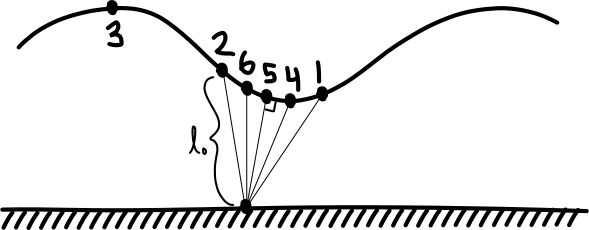
\includegraphics[width=0.6\textwidth]{Figures/SLIPSections}\par
\end{centering}
\caption[Diagram: SLIP Options for Poincare Sections]{SLIP options for Poincare sections. Various points in the gait cycle of the SLIP model can be used to generate a Poincare map. The section, or a particular slice of the periodic gait cycle, can fully define the motion. Each section is defined by a different occurence. Six different options are proposed, and option 3 is considered in more detail.}
\label{fig:SLIPSections}
\end{figure}
%

Though all of the options are valid, section \ref{item:MaxHeight} will be
analyzed here in further detail. This section reduces the four-dimensional
phase space using $x$, $y$, $\dot{x}$, and $\dot{y}$ to a three-dimensional
state space using only $x$, $\dot{x}$, and $y$ because it is known that
$\dot{y} = 0$ at the section slice. Additionally, we do not need to know $x$ in
order to predict the motion of the center of mass because the center of mass is
traveling only in the $x$ direction, and its location relative to the $x$-axis
is irrelevant if the motion is periodic. Getting rid of $x$ reduces our state
space to two dimensions. Given $y_{n}$ and $\dot{x}_{n}$, we want to predict
$y_{n+1}$ and $x_{n+1}$, where $n$ is an index through sequential
sections of the periodic motion.

Given the model and the free body diagram presented in section \ref{sec:SLIP},
we can calculate the trajectory of the center of mass. Such knowledge will
allow us to analyze the stability of SLIP motion. We can the trajectory with a
numerical ordinary differential equation (ODE) solver. Two such solvers are
MATLAB's ODE45 and ODE112. For the remainder of this section, we will describe
the simulation of the SLIP model in the context of MATLAB.

The SLIP model features three distinct segments of motion for the chosen
Poincare section. The first is the parabolic flight from the top of the
trajectory to where the leg initially touches the ground. This first segment of
motion is described by one set of differential equations. The second segment of
motion is the stance phase, in which the leg contacts the ground and the spring
is compressed. This segment is described by a different set of differential
equations. Finally, the third segment is again parabolic flight, described by
the same differential equations as the first segment. The transition between
the segments of motion can often be detected with an event detection feature of
the ODE solver, as is the case in MATLAB.

\begin{comment}
In the world of legged locomotion, it is important to analyze the stability of
locomotion models.
\end{comment}

Equipped with a choice for a Poincare section, we are almost ready to analyze
the passive stability of the SLIP model. We first require a stride function, or
return map, that describes how the center of mass changes state from $y_{n}$
and $\dot{x}_{n}$ to $y_{n+1}$ and $\dot{x}_{n+1}$.  For clarity in this
analysis, we define $q_{1}\equiv y_{n}$ and $q_{2}\equiv\dot{x}_{n}$. We also
define $\mathbf{q}$ as a vector of the two states $q_{1}$ and $q_{2}$, The
vector $\mathbf{q}_{n+1}$ is a function of $\mathbf{q}$, and so we define
$\mathbf{q}_{n+1} = \mathbf{f}(\mathbf{q})$.  We split the vector function
$\mathbf{f}(\mathbf{q})$ into two scalar functions, one for each state variable.

\begin{align}
q_{1,n+1}= f_{1}(q_{1,n},q_{2,n}) \notag \\
q_{2,n+1}=  f_{2}(q_{1,n},q_{2,n})
\label{eq:FullFunctionDefinition}
\end{align}

For a given $\mathbf{q}_{n}=[q_{1,n},q_{2,n}]^{T}$, the fixed point that
describes periodic motion occurs when
$\mathbf{q}_{n+1}=\mathbf{f}(\mathbf{q}_{n})=\mathbf{q}_{n}$. This fixed point
can be found using a method similar to that used to find the fixed point for
the motion of the rimless wheel. However for this problem, the calculations
will be performed in two dimensions, not one.

Given some kind of simulation that uses MATLAB's ODE solvers to calculate the
trajectory of the center of mass, We can obtain values for $q_{n}$ and
$q_{n+1}$ by simulating the motion using an ODE solver, as described above.
This provides us with an implicit definition of the function $\mathbf{f}$,
seeing as the ODE solver provides $\mathbf{q}_{n+1}$ from $\mathbf{q}_n$.
Equipped with $\mathbf{f}$, we can solve for the fixed point of the system
using a numerical nonlinear root-finder, such as MATLAB's FSOLVE.  However,
roofinders require that the problem takes the form $\mathbf{g}(\mathbf{q})=0$,
so we define a function $\mathbf{g}(\mathbf{q}) \equiv
\mathbf{f}(\mathbf{q})-\mathbf{q}$. To obtain periodic motion, the goal is to
solve for $\mathbf{q}$ such that $\mathbf{g}(\mathbf{q})=0$. This solution is
called the ``root'' and will be referred to here as $\mathbf{q}^{*}$.

 \begin{align}
 \begin{bmatrix}
 f_{1}(q_{1},q_{2}) \\
 f_{2}(q_{1},q_{2})
 \end{bmatrix}
 -
 \begin{bmatrix}
 q_{1} \\
 q_{2}
 \end{bmatrix}
 =
 \begin{bmatrix}
 0 \\
 0
\end{bmatrix}
\label{eq:GDefinition}
\end{align}


After solving equation \ref{eq:GDefinition}, it is desirable to know if the
motion is stable near this fixed point. To assess the stability of the fixed
point $\mathbf{q}^{*}$, the function $\mathbf{f}(\mathbf{q})$, must first be
linearized about $\mathbf{q}^{*}$.  This can be done with the first two terms
of a Taylor expansion:

\begin{equation}
    \mathbf{f} ( \mathbf{q} ) = \mathbf{f} ( \mathbf{q}^{*} ) +
    \frac{d}{d\mathbf{q}}\mathbf{f} (\mathbf{q}^{*}) ( \mathbf{q}
    - \mathbf{q}^{*} )
\label{eq:LinearShorthand}
\end{equation}

If the function $\mathbf{f}(\mathbf{q})$ is expanded, a matrix called the
Jacobian, $\mathbf{J}$, reveals itself. By examining the expanded form of the
Taylor approximation of $\mathbf{f}(\mathbf{q})$, it is easy to see why the
Jacobian determines the stability of the motion described by
$\mathbf{f}(\mathbf{q})$:

\begin{align}
\begin{bmatrix}
f_{1} (q_{1},q_{2}) \\
f_{2} (q_{1},q_{2}) 
\end{bmatrix}
=
\begin{bmatrix}
q_{1}^{*} \\
q_{2}^{*}
\end{bmatrix}
+
\begin{bmatrix}
\displaystyle\frac{\partial f_{1}}{\partial q_{1}} &  \displaystyle\frac{\partial f_{1}}{\partial q_{2}} \\
\displaystyle \frac{\partial f_{2}}{\partial q_{1}} & \displaystyle \frac{\partial f_{2}}{\partial q_{2}}
\end{bmatrix}
\begin{bmatrix}
\epsilon_{1} \\
\epsilon_{2}
\end{bmatrix}
\label{eq:LinearLonghand}
\end{align}

We define the Jacobian as

\begin{equation}
    \mathbf{J} = 
\begin{bmatrix}
\displaystyle\frac{\partial f_{1}}{\partial q_{1}} &  \displaystyle\frac{\partial f_{1}}{\partial q_{2}} \\
\displaystyle \frac{\partial f_{2}}{\partial q_{1}} & \displaystyle \frac{\partial f_{2}}{\partial q_{2}}
\end{bmatrix}
\label{eq:Jacobian}
\end{equation}



For the motion to be periodic, it has already been shown that
$\mathbf{f}(\mathbf{q})$ must equal $\mathbf{q}^{*}$. Any time a given step
$\mathbf{q}$ is given as input to the return map $\mathbf{f}(\mathbf{q})$, the
return map must output the input.  The $\mathbf{q}$ that accomplishes this is
called $\mathbf{q}^{*}$ by definition. If the input $\mathbf{q}$ deviates from
this ideal $\mathbf{q}^{*}$ and causes $\mathbf{f}(\mathbf{q})$ to output
something other than the input $\mathbf{q}$, the motion is considered stable if
the system eventually returns the ideal $\mathbf{q}^{*}$ after a few periods.

This can be seen by examining the second term on the right side of equation
\ref{eq:LinearLonghand}, where $\epsilon_{1}$ is the error associated with
$q_{1}$ and $\epsilon_{2}$ is the error associated with $q_{2}$. These errors
$\epsilon_{1}$ and $\epsilon_{2}$ represent a disturbance introduced by
variation in the terrain or environment of the hopping robot. Every time the
robot goes through one gait cycle, the errors $\mathbf{\epsilon}$ will change
from some initial disturbance $\mathbf{\epsilon}_{0}$, based on the difference
between \todo{epsilon bold is not working out!!} the fixed point
$\mathbf{\mathbf{q}}^{*}$ and the output $\mathbf{f}(\mathbf{q})$, and the
values of the elements in the Jacobian, $\mathbf{J}$.
\todo{this previous sentence can still be made a little clearer I think}
\todo{how is the Jacobian calculated? I guess from the physical equations?}

Though the values of the elements of the Jacobian do not change with each step
(or period), the change in the errors $\mathbf{\epsilon}$ causes the value of
the second term of the right side of equation \ref{eq:LinearLonghand} to either
shrink or grow with each step. Whethe the error shrinks or grows depends on
$\mathbf{J}$. If the errors $\mathbf{\epsilon}$ grow, so does the second term
of the right side of equation \ref{eq:LinearLonghand}, and the motion of the
hopper is unstable. So the important question is: does the initial perturbation
$\mathbf{\epsilon}_{0}$ grow? This can be determined by examining the
product of the Jacobian and the perturbation vector $\mathbf{\epsilon}_{n}$:

\begin{align}
\begin{bmatrix}
\epsilon_{1,n+1} \\
\epsilon_{2,n+1}
\end{bmatrix}
=
%\begin{bmatrix}
%J_{11} &  J_{12} \\
%J_{21} &  J_{22} 
%\end{bmatrix}
\mathbf{J}
\begin{bmatrix}
\epsilon_{1,n} \\
\epsilon_{2,n}
\end{bmatrix}
\label{eq:ErrorAndJacobian}
\end{align}

\todo[inline]{I changed an equation here quite a bit, replacing the 2x2 J with
just the matrix symbol for the Jacobian. This might make this section harder to
read cursorily quickly}

\begin{comment}
In equation \ref{eq:ErrorAndJacobian} the subscripts denote the associated
element of $\mathbf{f}(\mathbf{q})$.
\end{comment}

In the following analysis, subscripts denote the step in the simulation. It is
clear that $\mathbf{\epsilon}_{1} = \mathbf{J}\mathbf{\epsilon}_{0}$ and
$\mathbf{\epsilon}_{2} = \mathbf{J}\mathbf{\epsilon}_{1} =
\mathbf{J}\mathbf{J}\mathbf{\epsilon}_{0}$.  It follows then that
$\mathbf{\epsilon}_{n} = \mathbf{J}\mathbf{\epsilon}_{n-1} =
\mathbf{J}^{n}\mathbf{\epsilon}_{0}$.  The goal here is to discover if
$\mathbf{\epsilon}_{n}$ decays to zero as $n$ reaches infinity.  If that is
true, then the hopper is stable. By making use of the eigenvector definition,
the value of $\mathbf{\epsilon}_{n}$ as $n$ reaches infinity can be found:

\begin{equation*}
    J \mathbf{v} = \lambda \mathbf{v}
\end{equation*}

Given that for this problem, $\mathbf{J}$ is a $2 \times 2$ matrix, there are
two eigenvalues $\lambda_i$ and two corresponding eigenvectors $\mathbf{v}_i$
that satisfy the eigenvector definition:

\todo[inline]{We have an issue here with subscripts! I'm not sure how to
resolve this right now\ldots}

\begin{align*}
    \mathbf{J} \mathbf{\epsilon} =& \mathbf{J} (a_{1}\mathbf{v}_{1}+a_{2}\mathbf{v}_{2}) \\
=&a_{1}\lambda_{1}\mathbf{v}_{1}+a_{2}\lambda_{2}\mathbf{v}_{2}
\end{align*}

where

\begin{equation*}
    \mathbf{\epsilon} = a_1 \mathbf{v}_1 + a_2 \mathbf{v}_2
\end{equation*}

Generalizing for the $n$-th step gives the following:

\begin{equation*}
    J^{n}\mathbf{\epsilon} = \lambda_{1}^{n}a_{1}\mathbf{v}_{1}+\lambda_{2}^{n}a_{2}\mathbf{v}_{2}
\end{equation*}

which decays as $n$ reaches infinity for all $a_{1}$ and $a_{2}$ if and only if
$|\lambda_{1}| < 1$ and $|\lambda_{2}| < 1$.

\todo[inline]{The Jacobian does vary with time, right? but we currently say
otherwise.}

Now we know that we can determine if the motion of the SLIP system is stable by
looking at its eigenvalues. To do so, we need to know what the Jacobian is.
There are a few different ways to find the Jacobian.  The easiest way to
find the Jacobian is to have a root-finding program output the Jacobian when it finds the root $q^*$. MATLAB's FSOLVE can do this. Another way is to refer to
equation \ref{eq:LinearLonghand} and find the partial derivatives by taking a
limit:

\begin{equation}
\frac{\partial y}{\partial x}\bigg|_{x^{*}}
=\lim_{h \to 0} \frac{y(x^{*}+h)-y(x^{*})}{h}
\label{eq:FindingJacobian}
\end{equation}

Finally, one could find $\mathbf{J}$ by using an infinitesimally small value
$\delta$ to approximate the error in \ref{eq:FindingJacobian},
and solve for $\mathbf{J}$:

\todo[inline]{this used to say ``to approximate the partial derivatives''. did
i make a mistake by changing this?}

\begin{equation}
J= \frac{1}{\delta}
\begin{bmatrix}
    f_{1}\left(\mathbf{q}^{*}+\begin{bmatrix} \delta \\ 0 \end{bmatrix}\right)
        - f_{1}(\mathbf{q}^{*}) & f_{1}\left(\mathbf{q}^{*}+\begin{bmatrix} 0
            \\ \delta \end{bmatrix}\right) - f_{1}(\mathbf{q}^{*}) \\[3mm]

            f_{2}\left(\mathbf{q}^{*}+\begin{bmatrix} \delta \\ 0
            \end{bmatrix}\right) - f_{2}(\mathbf{q}^{*}) &
            f_{2}\left(\mathbf{q}^{*}+\begin{bmatrix} 0 \\ \delta
            \end{bmatrix}\right) - f_{2}(\mathbf{q}^{*})
\end{bmatrix}
\label{eq:FindingQStar}
\end{equation}

\todo[inline]{What is done in practice, is htis last result the easiest to
calculate, and it happens to be sufficiently accurate? What affects the
stability (initial conditions)}

We took three steps to determine if the SLIP motion is stable or unstable,
depending on the parameters used to define the model. This requires choosing a
Poincare section around which we can view the motion as periodic. Then, we
numerically define a function $\mathbf{f}(\mathbf{q})$ with which we can
determine the system's fixed point(s). By approximating
$\mathbf{f}(\mathbf{q})$ with a two-term Taylor series, we discover the
Jacobian matrix. By writing the Jacobian matrix using an eigenvalue
decomposition, we can determine if the system is stable or unstable around a
given fixed point.

\section{Simplest Walker} % (notes page 31-34)
\label{sec:SimplestWalker}
\index{simplest walker}

The rimless wheel model described in section \ref{sec:RimlessWheel} can be
modified logically in order to create a model of a simple bipedal gait. With
the rimless wheel, only two spokes at any given time are involved in the
interesting dynamics of the motion. Naturally, these two spokes can be thought
of as simple legs. In fact, Garcia \cite{garcia97} asserts that this model is
the simplest (irreducible) model of walking. As figure
\ref{fig:SimplestWalkerPendulum} hints, this model is a simplification of a
double pendulum model that was studied by others in the 1980's
\todo[inline]{need citation}. Indeed, this model contains two single pendula
rotating about the a single joint at the hip.

% FIGURE
\begin{figure}[h]		% h="here" t="top" b="bottom" p="separate page"
\begin{centering}
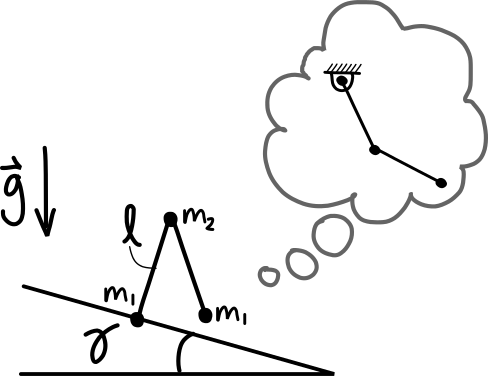
\includegraphics[width=0.5\textwidth]{Figures/SimplestWalkerPendulum}\par
\end{centering}
\caption[Diagram: Simplest Walker Model]{Simplest walker model. This model
consists of only two massless links of length $l$ joined at the hip, with
masses $m_{1}$ and $m_{2}$ at the ends of the links. For certain slopes of the
incline $\gamma$, stable motion is possible.}
\label{fig:SimplestWalkerPendulum}
\end{figure}
%

\subsection*{System description}
\label{sec:SimplestWalkerSystemDescription}

Similar to the rimless wheel model, the locomotive is traverseing an incline
defined by the angle $\gamma$. The leg that is in no-slip contact with the
incline is called the \textit{stance leg} and the other leg is called the
\textit{swing leg}\index{stance leg}\index{swing leg}. The legs are both
massless and have a length $l$. The mass of the hips is $m_{2}$, and the mass
of each foot is $m_{1}$, with $\beta = m_{1} / m_{2} \ll 1$.

% FIGURE
\begin{figure}[h]		% h="here" t="top" b="bottom" p="separate page"
\begin{centering}
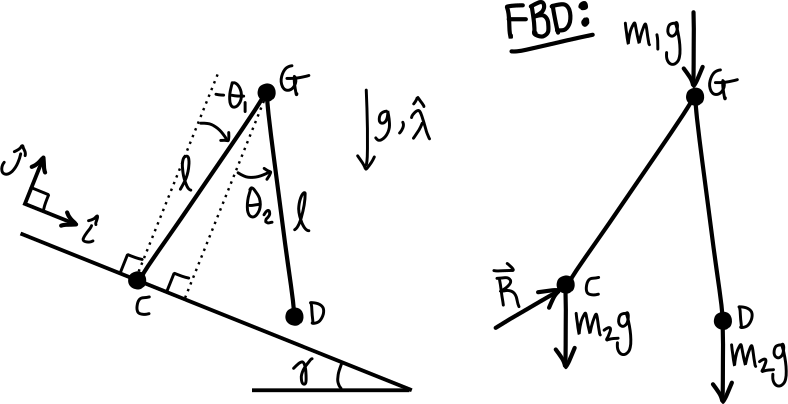
\includegraphics[width=0.8\textwidth]{Figures/SimplestWalkerFBD}\par
\end{centering}
\caption[Diagram: Simplest Walker Free Body Diagram]{Simplest walker free body diagram. The configuration of the model is defined by the rotations $\theta_{1}$ and $\theta_{2}$. Weights act at all three masses, and a ground reaction force acts at the contact point $C$.}
\label{fig:SimplestWalkerFBD}
\end{figure}
%

Unlike the rimless wheel, this system has two degrees of freedom because the
angle between the legs is not fixed. The configuration of the locomotive is
defined by the angles $\theta_1$ and $\theta_2$ and the corresponding angular
speeds $\dot{\theta}_1$ and $\dot{\theta}_2$. Both angles are defined with
respect to the normal of the incline. The free body diagram of the model in
figure \ref{fig:SimplestWalkerFBD} describes this locomotive in more detail.
The forces present in the full system are the weight of each mass and the
reaction force of the incline against the stance leg $\vec{\mathbf{R}}$ (the
vector sum of static friction and normal force). The motion proceeds under the
force of gravity. A free body diagram of the swing leg (not shown) would reveal
a force in the swing leg that is required to maintain the joint constraint at
point $G$. This force is decomposed into two components: tension $T$ along the
swing leg and a force $F$ perpendicular to the swing leg.

\todo{perhaps show an FBD of the swing leg}

\begin{comment}
[chris: in Alan's notes where is F's line of action?]
\end{comment}

\subsection*{Equations of Motion}
\label{sec:SimplestWalkerSystemDescription}

There are six unknowns in this model: the angular acceleration of each degree
of freedom, $\ddot{\theta}_{1}$ and $\ddot{\theta}_{2}$, the tension $T$ and
perpendicular force $F$ in the swing leg, and the two components of the support
force $\vec{\mathbf{R}}$. The system is described by two free body diagrams and
three momentum balances for each diagram. This gives six equations with which
we can solve for all six unknowns. To obtain only the motion of the locomotive
and avoid the support forces and internal forces, only angular momentum balance
is required for each of the two free body diagrams. For the full system free
body diagram, angular momentum balance about $C$ yields

\begin{align}
\Sigma \vM_{/C} &= \vHdot_{/C} \notag \\
(\vr_{G/C} \times m_{1} g  \ul ) + (\vr_{D/C} \times m_{2} g  \ul ) &= (\vr_{G/C} \times m_{1} \va_{G}) + (\vr_{D/C} \times m_{2} \va_{D})
\label{eq:SimplestWalkerAMB1}
\end{align}

where $ \ul $ is directed downward, in the direction of gravity.

Likewise, angular momentum balance of just the swing leg about $G$ yields

\begin{align}
\Sigma \vM_{/G} &= \vHdot_{/G} \notag \\
\vr_{D/G} \times m_{2} g  \ul  &= \vr_{D/G} \times m_{2} \va_{D}
\label{eq:SimplestWalkerAMB2}
\end{align}

To solve these equations, expressions for $\vec{\mathbf{a}}_{G}$ and $\vec{\mathbf{a}}_{D}$ are required.

\begin{align}
\va_{G} &= -\dot{\theta}_{1}^{2} \vr_{G/C} + \ddot{\theta}_{1} \uk \times \vr_{G/C} \\
\va_{D}  &= \va_{G} + \va_{D/G} \notag \\
 &= \va_{G}  -\dot{\theta}_{2}^{2} \vr_{D/G} + \ddot{\theta}_{2} \uk \times \vr_{D/G}
\end{align}

\todo[inline]{I'm not sure the signs for accelerations are correct here, since
theta's are defined positive for cw rotations}

where $\vr_{G/C} = l (- \sin{\theta_{1}} \ui +\cos{\theta_{1}} \uj)$ and
$\vr_{D/G} = l (\sin{\theta_{2}} \ui - \cos{\theta_{2}} \uj)$. The equations
can be greatly simplified if the feet have no mass, $\beta = 0$.


As with the rimless wheel, equations \ref{eq:SimplestWalkerAMB1} and
\ref{eq:SimplestWalkerAMB2} describe the dynamics of the model during the
smooth ``flight''. The solution for the smooth flight motion requires
information about the inelastic collision that occurs between flights. The
instant at which the collision starts is called
\textit{heelstrike}\index{heelstrike}. At heelstrike, point $C$ collides with
the incline and the collision is analyzed by the following equalities across
the collisions

\begin{align}
\vHdot_{/C}^{+} &= \vHdot_{/C}^{-} \notag \\
\vHdot_{/G}^{+} &= \vHdot_{/G}^{-} \notag
\label{eq:SimplestWalkerCollision}
\end{align}

These equations result in expressions that are very similar to equations
\ref{eq:RimlessHPlus} and \ref{eq:RimlessHMinus} for the rimless wheel, except
that this time there are two degrees of freedom to manage. As for the rimless
wheel, the weight of the masses can be ignored in the angular momentum
expressions since the collisions occur so quickly. The coupled differential
equations for $\theta_{1}$ and $\theta_{2}$ and the collision equations are
presented in \cite{garcia97}. \todo{we really don't want to show the derivation
here? I think there needs to be more meat here before we jump into
``stability'',
and our discussion on stability needs to align with our discussion of stability
from previous sections}

\subsection*{Bifurcation}
\label{sec:SimplestWalkerBifurcation}

The equations of motion in this model are actually
\emph{nonlinear}\index{nonlinear}. This means that for certain system
parameters the motion of the locomotive may be chaotic, and so small changes in
initial conditions can result in largely different motions. The simplest walker
model exhibits the \emph{period-doubling}\index{period-doubling} phenomenon as
the angle of the incline $\gamma$ is increased. The period-doubling is captured
in the bifurcation diagram\index{Poincare map} in figure
\ref{fig:SimplestWalkerEigenvalues}.

A bifurcation diagram is a graph in which the value of a state variable of the
model over many periods of the motion is plotted as a function of some
parameter of the model. The natural parameter to use in this case is the angle
of the incline $\gamma$. The vertical axis of this bifurcation diagram holds
the step length for each gait cycle. For small inclines, the step length is
constant for each gait cycle. This is shown in the graph, where there is only
one curve to the left of the dotted vertical line. The point where the curve
splits into two curves is called a \emph{bifurcation point}\index{bifurcation
point}.

\todo[inline]{step length is measured along the incline?}

% FIGURE
\begin{figure}[h]		% h="here" t="top" b="bottom" p="separate page"
\begin{centering}
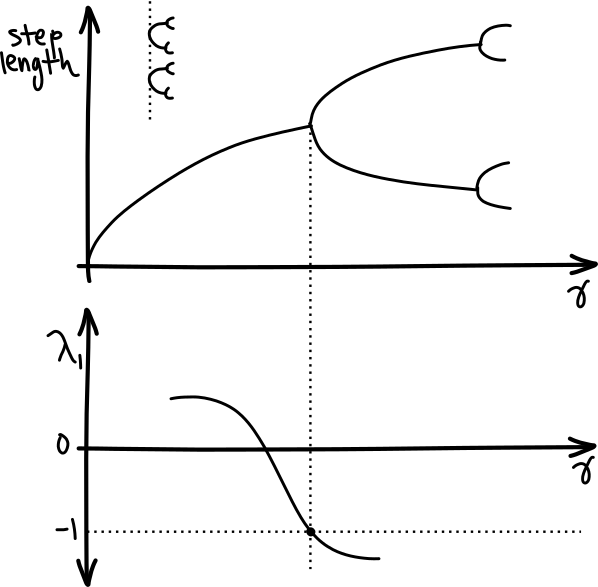
\includegraphics[width=0.6\textwidth]{Figures/SimplestWalkerEigenvalues}\par
\end{centering}
\caption[Plot: Simplest Walker Bifurcation and Eigenvalues]{Simplest walker
bifurcation and eigenvalues. The top plot is a bifurcation diagram that shows
the step length for many gait cycles for a given value of $\gamma$, as $\gamma$
is varied. The bottom plot shows the first eigenvalue of the Jacobian of the
system's Poincare map (map not shown). Eigenvalues of $\lambda = -1$ correspond
to bifurcation points, and consequently, \emph{period-doubling}. Beyond
$\gamma = \gamma^{*}$, the simplest walker executes a limping period-2 gait in
which step length alternates between two values.}
\label{fig:SimplestWalkerEigenvalues}
\end{figure}
%

\todo[inline]{figure: show 0.015 rad, or put in a variable for the gamma value
like gamma star. also, show arrows on the curves to show that they continue
on. Split figure into 4.12(a) and 4.12(b)}

The nonlinear behavior of the model is determined by the Jacobian of the
Poincare map. The first eigenvalue $\lambda$ of this Jacobian follows the curve
presented in figure \ref{fig:SimplestWalkerEigenvalues}. The values of $\gamma$
for which the eigenvalue $\lambda = -1$ are the incline angles at which
bifurcation occurs. After this bifurcation point, the motion is described as
being \textit{period-2}. This means that the step length alternates between two
values between gait cycles. This motion resembles limping, because one leg
takes larger steps than the other.

For $0 < \gamma < \gamma^{*}$ rad, the motion of the simplest walker model is
stable. The fact that such a simple mechanical model of locomotion has stable
solutions without actuation or control hints that the coordinated locomotion is
mostly mechanical. This view is in constrast with a view that states
coordinated locomotion results from muscle action or from neurological control
\cite{garcia97}.

For an in-depth description of the nonlinear behavior of this model, 
refer to Garcia \cite{garcia97}.


\section*{Passive Models of Locomotion}

All the models presented in this chapter and chapter
\ref{sec:ModelingLeggedLocomotion} are very simple. Mass has been concentrated
at the hip or at the foot. More detailed dynamic models of locomotion can be
developed in a somewhat logical fashion. The models can be extended by
including distributed masses for the legs, or perhaps links for the upper body.
For these situations, analytical descriptions quickly become cumbersome. It is
important though to examine if such detailed models add any new information or
provide any additional accuracy. There is an elegance to the ability to make
important conclusions about animal locomotion from the motion of only a few
point masses.


\begin{comment}
-eigenvalues less than one means stability.
-describe poincare/stability
-detail that dHdt vs Hdot only if C is not moving
-didnt talk about the passive nature of the locomotion
\end{comment}


%%%%%%%%%%%%%%%%%%%%%%%%%%%%%%%%%%%%%%%%%%%%%%%%

\chapter{Controlling Legged Locomotion}
\label{sec:ControllingLeggedLocomotion}
\index{control}

There are many different elements of legged locomotion control. This chapter covers two of the more well-known control algorithms: the first being a control algorithm based on the hopping robot from previous chapters, the second is a popular algorithm used by many robots in existence called the zero-moment-point method. The latter typically makes heavy use of motors placed at the joints that are being controlled to keep the center of mass of the robot in a desirable location, where the former uses a more dynamic placement-based method that keeps the robot's trajectory on a desired path.

%\section{Central Pattern Generator} % (notes page 67)
%\label{sec:CentralPatternGenerator}
%
%Central Pattern Generator: CPG. A collection of nerves that fire in sequence, generating "fictive locomotion" with no feedback from muscles. If the CPG were the whole story, locomotion would be feedforward. In reality, there is definitely feedback to the CPG.
%
%[ALAN] NEEDS MORE. Could be a very interesting section about the cat experiments from McMahon... I will have to hunt down that book somewhere here...

\section{Raibert Hopping Robot} %(notes page 34-39)
\label{sec:RaibertHoppingRobot}
\index{Raibert Robot}

Given the SLIP model of locomotion discussed in section \ref{sec:SLIP}, we want to know how we can control such a model. 

$I_{body}<<ml_{0}^{2}$: can't control $\theta_{c}$ in stance.
$I_{leg}<<I_{body}$: can control $\theta_{c}$ in flight.

Now let's assume compression in the spring is elastic: $E_{tot}$ = constant. The only control is $\theta_{c}$ at first contact. There are multiple approaches to control:

\subsection*{First Approach} Find a period solution. Given $l_{0}$, $k$, $m$, and $g$, find a $\theta_{c}^{*}$, $\dot{x}^{*}$, and $h^{*}$, at the apex of the hopper's flight, that will cause a motion that returns the hopper to the same conditions. Figure \ref{fig:SLIPPeriodicMotion} shows how we can find these initial conditions. By assuming symmetry about the apex of the motion, we can start the center of mass at its lowest point, with the spring compressed, and release it at a chosen velocity. If we then measure the angle at which the leg departs the ground, the height the center of mass reaches at the apex, and the forward velocity of the center of mass at the apex, we can use these quantities as our initial $\theta_{c}^{*}$, $\dot{x}^{*}$, and $h^{*}$.

% FIGURE
\begin{figure}[h]		% h="here" t="top" b="bottom" p="separate page"
\begin{centering}
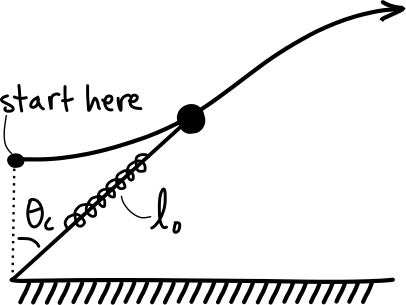
\includegraphics[width=0.4\textwidth]{Figures/SLIPPeriodicMotion}\par
\end{centering}
\caption[Diagram: SLIP Initial Conditions for Periodic Control]{SLIP initial conditions for periodic control. This diagram explains how to find initial conditions for the periodic method of SLIP control. If the motion is symmetric about the apex of the motion path, the initial conditions at the apex can be found by launching the mass from its lowest position at a chosen velocity.}
\label{fig:SLIPPeriodicMotion}
\end{figure}
%

However, this method of using periodic motion to control the locomotion of the hopper will likely be unstable. Nothing about this method of control indicates that the hopper will be able to reject disturbances in its gait. Previously, in section \ref{sec:SpringLoadedInvertedPendulum}, we briefly discussed using a linear controller to control the speed of the hopper: 

\begin{equation}
\theta_{c}=\theta_{c}^{*}+k(\dot{x}-\dot{x}^{*})+k_{2}(h-h^{*})
\label{eq:LinearController}
\end{equation}

In equation \ref{eq:LinearController}, the $k_{2}(h-h^{*})$ term is redundant because of energy conservation. 

***ASIDE ON EIGENVALUES was here in the notes. Page 36. Is it needed? I don't think it flows.***

\subsection*{Second Approach}

Insight and intuition. Raibert's way. Assume that energy is fixed. Observe that contact time, $T$, is almost independent of $\theta_{c}$. One can imagine that the hopper is simply a spring and a mass, fixed to the ground as shown in figure \ref{fig:SLIPCorrection}. The part of the trajectory of this spring-mass system that we care about is the lower half, which is analogous to the hopper's motion when the leg is touching the ground. This part of the motion of the hopper is assumed to be the same as this half-sine curve, with some correction made for the effect of gravity. 

% FIGURE
\begin{figure}[h]		% h="here" t="top" b="bottom" p="separate page"
\begin{centering}
\includegraphics[width=0.6\textwidth]{Figures/SLIPCorrection}\par
\end{centering}
\caption[Diagram: SLIP Height Correction for Raibert Control]{SLIP height correction for Raibert control. Height of the hopper is plotted in time through the stance phase of the SLIP motion, which is marked between the corrections. For Raibert control, the motion of the hopper in the stance phase is equivalent to that of a simple vertically oscillating mass-spring system. This results in a sinusoidal hopper height as a function of time with a correction for the constant acceleration due to gravity.}
\label{fig:SLIPCorrection}
\end{figure}
%

The sine curve can be described as

\begin{equation}
y=y_{0}+A\sin{\left(t\sqrt{k/m}\right)}
\label{eq:SineCurve}
\end{equation}

Since we only care about the bottom half of the sine curve, we can surmise the following:

\begin{equation}
T\sqrt{k/m}=\pi
\label{eq:SineArgument}
\end{equation}

But we must also consider the correction:

\begin{equation}
T=\pi\sqrt{m/k}+\mbox{correction}
\label{eq:ContactTime}
\end{equation}

Note here that $T$ is not the period of the sine curve, but the contact time of the leg on the ground. The period of the hypothetical sine curve of the hopper's motion would be $2T$.

Then, we observe that steady motions are symmetric in the stance phase of the total trajectory. This is shown in figure \ref{fig:SLIPSymmetry}. 

% FIGURE
\begin{figure}[h]		% h="here" t="top" b="bottom" p="separate page"
\begin{centering}
\includegraphics[width=0.45\textwidth]{Figures/SLIPSymmetry}\par
\end{centering}
\caption[Diagram: SLIP Symmetrical Stance Phase for Raibert Control]{SLIP symmetrical stance phase for Raibert controll. Since in the stance phase the height of the hopper is a sinusoidal function of time, the motion path is symmetrical. If the horizontal speed of the hopper is approximately constant, the width of the stance phase is $d = \dot{x}T$. This symmetry also allows for the painless calculation of $\theta_{c}$ requied to enforce this symmetry.}
\label{fig:SLIPSymmetry}
\end{figure}
%

Based on this assumption, we can derive a function that gives $\theta_{c}$ as a function of the horizontal speed of the center of mass of the hopper. To get that relationship, we first assume that the horizontal speed $\dot{x}$ is approximately constant throughout the entire gait cycle. This makes the calculation for $d$ trivial, $d=\dot{x}T$. From geometry then, we observe:

\begin{equation}
l_{0}\sin{\theta_{c}}=\frac{\dot{x}T}{2}
\label{eq:SLIPDistance}
\end{equation}

Since we are interested in $\theta_{c}$ as a function of $\dot{x}$, we solve equation \ref{eq:SLIPDistance} for $\theta_{c}$:

\begin{equation}
\theta_{c}=\arcsin{\left(\frac{\dot{x}T}{2l_{0}}\right)}
\label{eq:SLIPContactAngleBalance}
\end{equation}

Where $T$, the contact time, is found in equation \ref{eq:ContactTime}.

This derivation of $\theta_{c}$ is based entirely in the stance phase of the gait cycle, meaning all we have done is find a $\theta_{c}$ in terms of $\dot{x}$ that will keep the stance phase symmetric. Therefore we can think of this as a balance controller: given an initial forward velocity, the hopper will continue to go at that velocity, relatively unaffected by the balance controller's choice for $\theta_{c}$. To consider the linear speed controller that we found before, we simply add it to the balance controller:

\begin{equation}
\theta_{c}=\arcsin{\left(\frac{\dot{x}T}{2l_{0}}\right)}+k\left(\dot{x}-\dot{x}_{d}\right)
\label{eq:HopperController}
\end{equation}

K in this case must be small. This approach is similar to the first approach, but where the first has two free parameters, this tells us how to assign one of those parameters, $\theta_{c}$.

The second level of control: regulating energy level. First approach: measure E and add to it: $\mbox{energy}=k(E_{desired}-E)$. Second approach, Raibert style: dissipation per hop is monotonic in height. The dissipation per hop does not depend on the height of the hop. 

The third level of control: body orientation. Figure \ref{fig:SLIPBodyControl} shows the forces on a hopping robot's body that can be applied by motors. We can apply a moment on the leg during stance:

\begin{equation}
M=-k\theta_{b}-c\dot{\theta}_{c}
\label{eq:HopperBodyControl}
\end{equation}

% FIGURE
\begin{figure}[h]		% h="here" t="top" b="bottom" p="separate page"
\begin{centering}
\includegraphics[width=0.5\textwidth]{Figures/SLIPBodyControl}\par
\end{centering}
\caption[Diagram: SLIP Free Body Diagram for Control]{SLIP free body diagram for Control. A free body diagram for the SLIP model was presented in section \ref{sec:SLIP}. This free body diagram also includes a moment $M$ acting at the hinge which is used for leg angle control.}
\label{fig:SLIPBodyControl}
\end{figure}
%

Assume all three controls are effectively decoupled. Each applies a very small amount of noise to the other. 

Going back to the first approach: root finding to get a periodic solution. What if we didn't care about the hopper returning to its initial conditions on the first bounce, but rather we wished it to return to the initial conditions after two bounces? We can solve numerically for this, and we call it a ``period two'' solution. Figure \ref{fig:SLIPPeriodic} shows the trajectory of the state-space map. Period two solutions in legged locomotion are typically seen as a ``limp.'' 

Text from the notes that I don't really know how to make sense of: `` Or you could look at the period one solutions, at what happens when you do one perturbation, and you get an eigenvalue of neg. 1, then in 2 steps, you get back to where you were. ''

% FIGURE
\begin{figure}[h]		% h="here" t="top" b="bottom" p="separate page"
\begin{centering}
\includegraphics[width=0.4\textwidth]{Figures/SLIPPeriodic}\par
\end{centering}
\caption[Diagram: SLIP Periodicity and Limping]{SLIP periodicity and limping. The planes are phase-space planes. To the left is a description of typical systems, in which a operates at a single fixed point, and the system has the same state at the same point in any two periods. To the right is a description of a system operating in period 2, in which the state of the system alternates between two solutions at the end of each period. In the context of locomotion, this latter case is typically a model for limping gaits.}
\label{fig:SLIPPeriodic}
\end{figure}
%

\section{ZMP and Capture Point Method} %(notes page 60-64)
\label{sec:ZMPAndCapturePointMethod}
\index{ZMP}
\index{capture point method}

One popular method used to control modern legged robots is the zero-moment-point (ZMP) method. Honda's Asimo robot is a good example of a robot whose gait dominated by this method of control. Before getting into the details of this method of control, it is important to understand the basic result of using the ZMP method. Imagine a bipedal walking robot that uses the ZMP method of control. At any point in its gait, freeze the robot and lock all of its joints. Neglecting the momentum of the limbs, if the robot were frozen at any point in its gait, it would be able to stand. Each frozen frame of the robot's gait is a statically stable position because there is no \textit{net moment} on the robot's body. 

The method of control requires careful control of the joint angles. It also requires that the feet have some surface area that makes complete contact with the ground. In other words, the feet of the robot must be completely flat to make use of the torques produced at the joints. 

The basic program for operation of a robot that uses ZMP control starts with specifying all the joint angles of the robot as a function of time. This means that almost everything about the state of the system and its centers of mass is known. The velocities, joint forces, acceleration, torques, etc. can all be calculated. To calculate the forces in the system, an open kinematic chain can be used. Start with an open limb, like a hand, and do the free body diagram and momentum balances for it. Once the forces acting on the hand are calculated, the forces on the connecting limbs can also be calculated. 

%%
%% Vukabrotovic 1968,2004.
%%

The two-dimensional feet shown in figure \ref{fig:ZMPFoot} are statically equivalent. Since the ground only pushes upwards on the foot, all realizable force distributions have a ZMP inside the foot. The figure shows where the name ``Zero Moment Point" comes from; the ZMP is the point on the foot where the net force vector can be moved such that no net moment is exerted on the foot. 

% FIGURE
\begin{figure}[h]		% h="here" t="top" b="bottom" p="separate page"
\begin{centering}
\includegraphics[width=0.5\textwidth]{Figures/ZMPFoot}\par
\end{centering}
\caption[Diagram: Zero Moment Point at Foot]{Zero moment point control at foot. An equivalent force system exists such that only a resultant force exists, and acts a so-called zero moment point. The location of the ZMP is determined by selecting a value for $\theta_{i}(t)$.}
\label{fig:ZMPFoot}
\end{figure}
%

One way of programming a robot to walk with a stable motion that uses this concept is to start with a specified joint angle control scheme in time, $\theta_{i}(t)$ and calculate the resulting ZMP at the foot. Then, check that the ZMP is always inside the outline of the foot. If the ZMP is not inside the foot, try different joint angle control scheme $\theta_{i}(t)$. However, this control strategy is incomplete. To find a working $\theta_{i}(t)$, the process needs to be repeated until a working $\theta_{i}(t)$ appears, which could take considerable time. It is helpful to know \textit{how} to change $\theta_{i}(t)$ such that we get a control scheme where the ZMP is always inside the foot. 

Consider a person standing in one place, as in figure \ref{fig:ZMPPerson}. In this diagram, C is the zero moment point. D is the desired location of the zero moment point. G is the point on the foot which is directly below the person's center of gravity. To stand still, G must equal C.

% FIGURE
\begin{figure}[h]		% h="here" t="top" b="bottom" p="separate page"
\begin{centering}
\includegraphics[width=0.2\textwidth]{Figures/ZMPPerson}\par
\end{centering}
\caption[Diagram: Zero Moment Point Control for Humans]{Zero moment point control for humans. The point $C$ is the ZMP, the point $G$ is located at the horizontal position of the center of mass, and the point $D$ is a desired location of the ZMP for control purposes. When $C$ and $G$ are at the same point, the human can stand still.}
\label{fig:ZMPPerson}
\end{figure}
%

Taking an angular momentum balance with respect to C, the average system rotation is in the direction of C to G. For example, the sum of the moments with respect to C is in the counter-clockwise direction. If $\vHdot_{/G'}$ is negligible, G accelerates away from C:

\begin{equation}
\vHdot_{/C}=\vr_{G'/C}\times\va_{G'}m+\vHdot_{/G'}
\label{eq:ZMPAMB}
\end{equation}

So an appropriate balance scheme is the following: place C so that G is between C and D, and G moves towards D as a result. Given that there is a force at the ankle, the ankle torque directly controls the location of C. This is a similar control scenario as the torque control of an inverted pendulum. 

%%
%% Perhaps expand upon the inverted pendulum stuff...
%%

Now consider a person walking. A similar ZMP control strategy to the one applied to standing can also be used for walking. The first step in a ZMP walking control strategy is to generate a trajectory of the robot and all the joints such that the ZMP is always inside the convex hull of the feet. The convex hull of the feet is illustrated by figure \ref{fig:ConvexHull}; it is the region of minimum perimeter that includes the outlines of both feet. When there is only one foot on the ground, the convex hull of the feet is the same as the outline of one foot. 

% FIGURE
\begin{figure}[h]		% h="here" t="top" b="bottom" p="separate page"
\begin{centering}
\includegraphics[width=0.3\textwidth]{Figures/ConvexHull}\par
\end{centering}
\caption[Diagram: Convex Hull of Feet]{Convex hull of feet. This diagram shows both feet in a top down view, and both feet are contacting the ground. The shaded area is the convex hull of the feet, which is the minimum-perimiter closed linear spline that includes both feet. If only one foot is on the ground, then the convex hull is the outline of only that one foot. For ZMP control, the zero moment point must be within the convex hull at all times.}
\label{fig:ConvexHull}
\end{figure}
%

The next step in a ZMP walking control strategy is to apply it to a robot and correct errors if the measured C does not equal D. There are three ways to correct for such errors. The first is corralling like for standing; however, this strategy doesn't work if G is outside of the convex hull. The second way to get C to equal D is to quickly bend the body to move the center of mass and exert a force at the feet. The third way is to adjust a step the robot was going to take anyway. The robot should take a bigger step if falling unintentionally forwards, and smaller if falling backwards. This is where the concept of capture regions comes from. A capture region is a set of places that a robot can put its foot and then find a control strategy that will allow it to end up standing still, given that the robot is already falling from one foot to the other.

%%
%% Cite Jerry Pratt for something in here. 
%% I had also wanted to mention something about stilts in here. 
%%



%%%%%%%%%%%%%%%%%%%%%%%%%%%%%%%%%%%%%%%%%%%%%%%%

\chapter{Energetics of Locomotion}
\label{sec:EnergeticsOfLocomotion}
\index{energetics}

In this book, the description of locomotion has been grounded in understanding the relevant dynamics through energy. Chapter \ref{sec:Introduction} introduced the cost of transport $COT$ as a metric for locomotion. Chapter \ref{sec:PropertiesOfMotorsAndMuscles} describes the peak power that muscles can produce, and introduces the metric of \textit{metabolic cost}. The models developed in chapter \ref{sec:ModelingLeggedLocomotion} include discussions of metabolic cost and energy loss from collisions.

Energy is such an important aspect of locomtion because it seems that locomotives may move in such a way as to minimize the metabolic cost of locomotion. Likewise, the metabolic cost can be minimized for the models of locomotion presented in this text. If the metabolic cost of locomtion is available for a given dynamics model of locomotion, then it may be possible to determine the parameters of the model that minimize that cost. These ideas are explored in chapter \ref{sec:OptimizationInLocomotion}. This chapter serves to bridge the topics that have been explored already to the ideas of energy optimization by providing a more thorough background in energy and muscle work.

\section{Power for Mechanical Systems} %(notes page 39, 43-49)
\label{sec:PowerforMechancialSystems}

This section contains a review of some fundamental ideas in classical dynamics, and moves onto some thermodynamics and a description of muscles that extends beyond what was presented in Chapter \ref{sec:PropertiesOfMotorsAndMuscles}.

The systems considered in introductory dynamics courses often do not require one to consider internal forces. This is fine, because it is only the external forces and torques that must be present in equations of momentum balance. After all, internal forces do not appear in free body diagrams.  Internal forces are usually more relevant in a statics course, or for analyzing failure of a system; they are not required for determining rigid body motion with momentum balance.  However, internal forces are relevant when using energy and power to describe motion.  Accordingly, a locomotive's motion depends on both internal forces and external forces. The free body diagram of a car only includes external forces, such as gravity, normal forces, and friction. The internal forces do not appear in a free body diagram of the entire car, but would appear in a free body diagram of just the engine, or of just the transmission (figure \ref{fig:CarForces}).

% FIGURE
\begin{figure}[h]		% h="here" t="top" b="bottom" p="separate page"
\begin{centering}
\includegraphics[width=0.3\textwidth]{Figures/CarForces}\par
\end{centering}
\caption[Diagram: Forces in and on a car]{Forces in and on a car. During typical operation, a car has both internal forces and external forces acting upon it. The internal forces may arise from the transmission or the passengers, while the external forces consists of gravity, ground reaction, and friction.}
\label{fig:CarForces}
\end{figure}
%

Humans, animals and robots are like cars in that they are not propelled solely by external forces (such is the case with point masses). What implications does this have for energy, and more intuitively, power? It is enlightening to develop equations for power with a distinction between internal and external forces. The instantaneous power required to force a particle that is traveling at a velocity $\vv$ is

\begin{align}
\vF_{tot} \cdot \vv  &=  m\va \cdot \vv = \frac{d}{dt} \left(\frac{m v^2}{2}\right) \\
 P &= \KEdot
\end{align}

where the chain rule of differentiation has been employed, $d(v^{2})/dt = 2v(dv/dt)$. This provides the logical work-energy theorem result for a particle, that $P = \dot{\KE}$. Of course in this case the total force is also the total external force, since a single particle cannot have any internal forces.

The power required to move a collection of particles, or a system of particles and rigid bodies, is

\begin{align}
 \sum_{i} \vF_{i} \cdot \vv_{i}  &=  \sum_{i} \frac{d}{dt}\left(\frac{m_{i} v_{i}^{2}}{2}\right) = \sum_{i} \KEdot_{i}\\
P^{tot} &= \KEdot
\label{eq:PowerCollectionOfParticles}
\end{align}

where $\vF_{i}$ is the total force on particle $i$ whose velocity is $\vv_{i}$, and $\KEdot$ is the time rate of change of the system's total kinetic energy. Equation \ref{eq:PowerCollectionOfParticles} can be used to describe the power developed with a system as simple as a two-particle system, or as complicated as a car. In the latter case, the system is comprised mostly of rigid bodies, in which case the forces and velocities are of the centers of mass of the rigid bodies.

As we mentioned, it is important to make a distinction between internal and external forces. Consider a collection of particles (no rigid bodies). The total force on particle $i$ can be split up as $\vF_{i} = \vF_{i}^{int} + \vF_{i}^{ext}$. If we make this distinction, the power can be written as the sum of an internal power and an external power.

\begin{align}
P^{tot} &= \sum_{i} (\vF_{i}^{int} + \vF_{i}^{ext}) \cdot \vv_{i} = P^{int} + P^{ext}\\
P^{int} &= \sum_{i} \vF_{i}^{int} \cdot \vv_{i} \\
P^{ext} &= \sum_{i} \vF_{i}^{ext} \cdot \vv_{i}
\end{align}

The power-\.{energy} relationship is then

\begin{align}
P_{tot} &=  \KEdot\\
P^{int} + P^{ext} &= \KEdot_{/G} + \KEdot_{G}
\label{eq:PowerInternalExternal}
\end{align}

where $\KEdot_{/G}$ is the time derivative of the sum of the kinetic energy of each particle with respect to the center of mass of the system, and $\KEdot_{G}$ is the time derivative of the kinetic energy of the center of mass of the system. Accordingly, these last two terms are

\begin{align}
\KEdot_{/G} &= \frac{d}{dt} \sum_{i} \frac{m_i}{2}(v_{i} - v_{G})^{2} = \frac{d}{dt} \sum_{i} \frac{m_i}{2} v_{i/G}^{2} \\
\KEdot_{G} &= m_{T} \frac{d}{dt} v_{G}^{2}
\end{align}

where $v_{G}$ is the speed of the center of mass of the system, and $m_{T} = \sum m_i$ is the total mass of the system. These two equations come from Konig's theorem, equation \ref{eq:Konig}, which was derived in \ref{sec:EquationsOfMotion}. We arrived at equation \ref{eq:PowerInternalExternal} by working with power rather than work because the math for power is simpler. For a formulation that starts with work instead, refer to the classical dynamics text by Greenwood \cite{greenwood}.

Equation \ref{eq:PowerInternalExternal} describes power through a sum of internal forces and external forces, and describes the time rate of change of kinetic energy as a sum of a ``relative'' kinetic energy, and a center of mass kinetic energy. It may seem that these terms correspond to each other; that the internal forces cause an internal power equivalent to $\KEdot_{/G}$ and that the external forces cause an external power equivalent to $\KEdot_{G}$. For example, if a car is in neutral and the driver depresses the accelerator, then the car has internal forces that contribute to an internal power that \textit{is} equivalent to $\KEdot_{/G}$ since the engine does turn. There is no external power since the external forces ground reaction act at stationary points and $\KEdot_{G} = m_{T}(0)^2/2 = 0$. The proposed correspondence holds.

However, this correspondence is incorrect in general. Consider the car in figure \ref{fig:CarForces} once again. A free body diagram of this car illustrates that if the car is accelerating, its acceleration is a result of the horizontal external force acting at the bottom of its wheels. Additionally, $\KEdot_{G}$ is increasing since it is a function of $v_{G}$. While this external force is necessary to give rise to $\KEdot_{G}$, this force does not create the power that contributes to $\KEdot_{G}$. The velocity of a wheel at the point at which the horizontal external friction force is instantaneously zero from the no-slip condition. Thus, this external force does not produce any power. Instead, the relation between external force and $\KEdot_{G}$ is developed by first noting that

\begin{equation}
\KEdot_{G} = \frac{d}{dt} \KE_{G} = m_{T}  \frac{d}{dt} (\vv_{G} \cdot \vv_{G}) = m_{T} \va_{G} \cdot \vv_{G}
\end{equation}

and then by dotting Newton's second law with $\vv_{G}$

\begin{align}
( \vF^{ext} &= m_{T} \va_{G} ) \cdot \vv_{G} \\
\vF^{ext} \cdot \vv_{G} &= \KEdot_{G} \label{eq:CarExternalForce}
\end{align}

The left hand side of equation \ref{eq:CarExternalForce} is \emph{not} external power (the term is revisited later), but nonetheless the external force can be seen to relate to the center of mass kinetic energy of the car. The internal forces that generate power that contribute to $\KEdot_{G}$ are in the engine, the transmission, and so on. While it is possible to develop physically meaningful conceptions of mass, acceleration, force, and kinetic energy, the left hand side of equation \label{eq:CarExternalForce} has no perceptible conceptual or physical meaning.

We elucidate this distinction by using one of the simplest systems of particles possible, as described in figure \ref{fig:ParticleExplosion}. Two masses are attached to each other by a spring with spring constant $k$, and the right mass is fixed to a wall. The system is excited, and the left mass oscillates. The center of mass of the two particle system is located at the midpoint between the masses. There is an external reaction force from the surface on the right particle, $F_{ext}$ that enforces the fixed constraint on the right mass.

% FIGURE
\begin{figure}[h]		% h="here" t="top" b="bottom" p="separate page"
\begin{centering}
\includegraphics[width=0.4\textwidth]{Figures/ParticleExplosion}\par
\end{centering}
\caption[Diagram: Two Masses on a Spring]{Two masses on a spring. Two masses are attached to each other by a spring with spring constant $k$, and the right mass is fixed to a wall. This simple example can illustrate how  internal and external power contribute to the kinetic energy of a system of particles. The external reaction force acts at a stationary mass, and thus does not produce any power. It is rather the internal power generated by the spring force that gives rise to the kinetic energy of both the left mass and the system of particles.}
\label{fig:ParticleExplosion}
\end{figure}
%

In this example, it is clear that $\KEdot_{G}$ is nonzero, since the center of mass has motion, but this motion arises from the power developed by the internal spring force $k\Delta x$, not from the external reaction force $F_{ext}$. The external reaction force acts at a stationary point, and thus does not develop any power. In the limit as $m_L/m_R \rightarrow \infty$, the system becomes a single oscillating mass, and the internal work becomes equivalent to the center of mass kinetic energy.

Thus, the relation between internal power, external power, ``relative'' kinetic energy and center of mass kinetic energy is more elusive than it may seem at first.

\subsection*{Power in Biomechanics}
\label{sec:Power in Biomechanics}
\index{external power}

In biomechanics, the terms ``internal power'' and ``external power'' do not
refer to the terms $P^{int}$ and $P^{ext}$ as they have been defined in this
text. We can clarify this difference for systems of point masses (no rigid
bodies). The biomechanics internal power $P_{bio}^{int}$ and external power
$P_{bio}^{ext}$ are defined by

\begin{align}
P_{bio}^{int} &= \sum_{i} F_{i} \cdot \vv_{i/G} \\
P_{bio}^{ext} &= \sum_{i} F_{i}^{ext} \cdot \vv_{G} = \vv_{G} \cdot \sum_{i} F_{i}^{ext}
P^{tot} &= P_{bio}^{int} + _{bio}^{ext} \\
\end{align}

The biomechanics internal power is the sum across particles of the \emph{total}
force on each particle multiplied with its velocity \emph{relative to the
center of mass}. The biomechanics external power is the sum across particles of
the total external force on each particle multiplied with the velocity of the
entire system's center of mass. This is equivalent to treating the system as a
single point mass with velocity $v_{G}$ and with a total external force
$F^{ext} = \sum F_{i}^{ext}$ acting upon it.

The biomechanics power terms have the nice feature that

\begin{align}
P_{bio}^{int} &= \KEdot_{/G} \label{eq:PbioInt}  \\
P_{bio}^{ext} &= \KEdot_{G}  \label{eq:PbioExt}
\end{align}

However, this is the extent of the usefulness of the biomechanics usage of internal power and external power. Additionally, 

\begin{itemize}
\item The definition of power requires that in the term $\vF \cdot \vv$, the
    force $\vF$ acts at the point which has velocity $\vv$. This is not true
    for $P_{bio}^{ext}$, since external forces do not necessarily act at the
    center of mass of a system (the system may not even have physical material
    at the center of mass).
\item The biomechanics power definitions cannot be related to the power
    generated by actuators or muscles.
\item The mechanics power definitions have the benefit that to evaluate power,
    the velocities of points at which no force is applied do not need to be
    known. If the force at a point $F_{i}$ is zero, then $F_{i}\cdot\vv_{i} = \mathbf{0} \cdot \vv_{i} =
    0$.
\item $P_{bio}^{int}$ is never useful and never provides any insights, and also counterintuitively depends on external forces.
\item $P_{bio}^{ext}$ is only useful for particle models.
\end{itemize}

In the biomechanics literature, the phrases ``internal power'' and ``external
power'' are often confused as referring to the terms $P^{int}$ and $P^{ext}$,
while the phrases actually refer to the $P_{bio}^{int}$ and $P_{bio}^{ext}$.
Keep in mind that the discussion here focuses on particle systems, and not
systems of rigid bodies.

\subsection*{Rigid object systems}

A locomotive can be approximated as a system of linked rigid bodies. Potentially, a locomotive is modeled better as a system of linked rigid bodies than as a collection of point masses, especially if the aim is to understand how muscles affect the motion of the locomotive. The time rate of change of the total kinetic energy of a locomotive $\KEdot$ can be expressed in terms of the forces and moments acting on the rigid bodies that compose a locomotive in a way that is slightly more detailed than equation \ref{eq:PowerInternalExternal}.  Again, the locomotive can have both internal and external forces. Starting from equation \ref{eq:PowerInternalExternal} and noting that $\vv_i = \vv_{G} + \vv_{i/G}$ and $\vv_{i/G} = \vomega_{G} \times \vec{\mathbf{r}}_{i/G}$, the power-\.{energy} relation is

\begin{align}
\KEdot &= P^{tot} \notag \\
 &= \sum_{i} (\vF_{i}^{int} + \vF_{i}^{ext} ) \cdot ( \vv_{G} + \vomega_{G} \times \vec{\mathbf{r}}_{i/G})
\end{align}

The right hand side can be expanded, and one of the resulting terms is

\begin{equation}
\sum \vF_{i}^{int} \cdot (\vomega_{G} \times \vec{\mathbf{r}}_{i/G}) \notag
\end{equation}

Using vector properties, this term can be rewritten as

\begin{equation}
\vomega \cdot \sum \vec{\mathbf{r}}_{i/G} \times \vF_{i}^{int} \notag
\end{equation}

This term vanishes, since according to Newton's second law, each internal force on a link also has an equal and opposite force acting on some other link. Through other simplifications, the power-\.{energy} relation eventually becomes

\begin{equation}
\KEdot = \sum_{i} \vF_{i}^{ext} \cdot \vv_{i} + \sum_{i} \vomega_{G} \times \vM_{i}^{ext}
\end{equation}

where $\vM_{i}^{ext}$ is the total external moment on link $i$. Thus, the energy of a rigid body system only depends on external forces and external moments. This conclusion seems to contradict the earlier statement that indicates that the kinetic energy of the center of mass of the system can recieve contribution from internal forces and internal power. [chris: doesn't it?] Consult any standard advanced dynamics textbook for a more thorough understanding of this derivation.

\section{Thermodynamics of Locomotives}
\label{sec:ThermodynamicsofLocomotives}
\index{thermodynamics}

In the context of internal forces an internal power, it makes sense to apply to the First Law of Thermodynamics to a model of a locomotive. Thermodynamics is particularly useful when trying to perform experiments on locomotives: how can metabolic cost be measured? Answering such a question requires knowledge of the ways that energy flows about a body. Previously, we have only dealt with the total \emph{mechanical} energy. The total energy of a locomotive, which is a closed system, is the sum of its kinetic energy $\KE$ and its internal energy $U$. Potential energy is neglected. The time rate of change of the total energy of a locomotive is

\begin{equation}
\KEdot + \dot{U} = P^{ext} + \dot{Q} + \dot{W}
\label{eq:Thermodynamics1}
\end{equation}

The external power $P^{ext}$ arises from friction, the heat input term $\dot{Q}$ arises from temperature differences, and the work term $\dot{W}$ arises from external work input to the system. Friction and the work term can be neglected, since sliding does not often occur with locomotives and so no power is lost to friction, and no odd external work inputs are considered. The time rate of change of the internal energy of the locomotive is

\begin{equation}
\dot{U} = -P^{int} + [\mbox{heat source}] + \dot{E}_{chem}
\label{eq:Thermodynamics2}
\end{equation}

The power terms are logically separated along the internal-external divide: the internal power is part of the time derivative of the internal energy. The $P^{int}$ term must have a negative sign in front of it to remain consistent with equation \ref{eq:PowerInternalExternal}, but because any energy used to do work inside the system must obtain that energy from the system. In the example of the car, the internal power in the engine related with the force of combustion products against piston heads comes from decreasing the enthalpy of the combustion products. For familiarity, the heat production term is commonly expressed in heat transfer texts as $\dot{q}'''V$, a heat production density multiplied by a volume. This can come from internal friction of body parts, but more likely from the heat produced by the inefficiency of thermodynamic processes. The chemical energy $\dot{E}_{chem}$ is the useful energy that is made available by the processing of chemicals such as ATP or fat. It is this term that is related to the oxygen consumption of animals that is often used to measure the metabolic cost of locomotion.

Combining equations \ref{eq:Thermodynamics1} and \ref{eq:Thermodynamics2}, the assumptions for $P^{ext}$ and $\dot{W}$, and expanding the kinetic energy term provides

\begin{equation}
P^{int} + (\dot{Q} - [\mbox{heat prod}]) - \dot{E}_{chem} = \KEdot_{/G} + \KEdot_{G}
\end{equation}

Typically, $\dot{Q} < 0$ since the body is at a higher temperature than the surrounding atmosphere, and $\dot{E}_{chem} < 0$ so that energy is removed from the internal energy of the body and is made useful as kinetic energy. The heat flow terms have been grouped to provide a net heat flow term for clarity.

\section{Locomotives and Muscle Power}
\label{sec:LocomotivesAndMusclePower}
\index{muscle power}

The general ideas presented so far can now be applied in a more direct fashion to humans and animals. Just as the engine in an automotive gives rise to internal forces and power that ultimately move the automobile, the muscles in an animal give rise to internal power that move the locomotive. The following assumptions and simplifications are made

\begin{itemize}
\item \textbf{Negligible gravity power:} Logically, this text is only concerned with mostly horizontal translation of the locomotion's center of mass. Thus, the force of gravity does not create a substantial external power (the force of gravity is perpendicular to the center of mass's velocity, and so the dot product of the two quantities is small). This would not be true for locomotion down or up a substantial incline.
\item \textbf{Negligible friction power:} Energy is not removed from the system (the locomotive) by either air friction or sliding. Sliding can occur, but only for a frictionless contact.
\item \textbf{Negligible ground deformation:} Energy is not removed from the system as a result of the collisions of limbs with the ground.
\end{itemize}

To a large extent, these assumptions are made so that the $P^{ext}$ term in the thermodynamic energy balance can be neglected. Additionally, internal friction is also neglected. Internal friction can come from frictional joints or from the inelastic compression of non-muscle soft tissue. As a result, the only relevant power source (or sink) in the system is the internal power generated by muscles or by joints in the locomotive. That is,

\begin{equation}
P = P^{int} + \cancel{P^{ext}} = \sum_{i} P_{i}^{joint} + \sum_{j} P_{j}^{musc}
\end{equation}

A joint, such as an elbow, can be analyzed by first developing a free body diagram of the joint, as in figure \ref{fig:ElbowFBD}.

%
% FIGURE
\begin{figure}[h]		% h="here" t="top" b="bottom" p="separate page"
\begin{centering}
\includegraphics[width=0.8\textwidth]{Figures/ElbowFBD}\par
\end{centering}
\caption[Diagram: Free Body Diagram of an Elbow]{Free body diagram of an elbow. To analyze an animal's joint using mechanics, the physical model of the joint (including bones and muscles) is reduced to a free body diagram with a single force-couple system in at the joint.}
\label{fig:ElbowFBD}
\end{figure}
%

The muscle can be modeled as a spring that acts between two points on different bones. There are likely many forces acting on a joint, but they can be reduced to an equivalent single force and moment. The power generated at the joint is then given by the resultant moment and the angular velocity at which the joint is opening or closing.

\begin{equation}
P_{i}^{joint} = \vM \cdot \vomega_{rel}
\end{equation}

% FIGURE
\begin{figure}[h]		% h="here" t="top" b="bottom" p="separate page"
\begin{centering}
\includegraphics[width=0.3\textwidth]{Figures/TwoJoints}\par
\end{centering}
\caption[Diagram: Two-Joint Muscles]{Two-joint muscles. Some muscles act through two joints via a tendon, and accordingly the power generated by the muscle is exprssed differently than for muscles that act across only one joint.}
\label{fig:TwoJoints}
\end{figure}
%

Some muscles act through two joints, as shown in figure \ref{fig:TwoJoints}. In this case, the muscle is connected to the farther bone through a tendon. The power generated by the muscle is approximated by

\begin{equation}
P_{i}^{musc} = - T \dot{l}
\end{equation}

where $T$ is the tension in the muscle and $l$ is the length of the muscle, as in figure \ref{fig:OneMuscle}.

% FIGURE
\begin{figure}[h]		% h="here" t="top" b="bottom" p="separate page"
\begin{centering}
\includegraphics[width=0.4\textwidth]{Figures/OneMuscle}\par
\end{centering}
\caption[Diagram: Muscle tension]{Muscle tension. The power generated by a muscle can be expressed as the product of the tension in the muscle and the rate of its elongation.}
\label{fig:OneMuscle}
\end{figure}
%
[chris: this would be a good place to dicuss concentric and eccentric contractions]
By analyzing muscles in this way, it is possible to quantify the overall level of muscle activity occuring in a locomotive. This provides an ``inside-out'' method of calculating the power generated by the muscles of a locomotive. Logically, this ``inside-out'' method is more arduous and riddled with complexity than perhaps an outside observation of energy usage.

\section{Measuring Power}
\label{sec:MeasuringPower}
\index{measuring power}

We can deductively determine the muscle activity by finding $P^{int}$ externally, through experiments. The simplest type of experiment is having a locomotive perform a gait on a force plate, as shown in figure \ref{fig:ForcePlate}. A likely setup is to place the force plate under a tread mill on which the locomotive moves in place. The force plate then records the vertical force exerted by the locomotive $\vF^{tot}(t)$ as a function of time.

% FIGURE
\begin{figure}[h]		% h="here" t="top" b="bottom" p="separate page"
\begin{centering}
\includegraphics[width=0.25\textwidth]{Figures/ForcePlate}\par
\end{centering}
\caption[Diagram: Force Plate]{Force plate. A force plate is used to measure the force that a locomotive exerts on the ground during its locomotion. It is possible to use a force plate to estimate the power usage of a locomotive. Multiple force plates can be used (perhaps one per foot) to obtain more detailed results.}
\label{fig:ForcePlate}
\end{figure}
%

The recorded force can be divided into two parts.

\begin{equation}
\vF^{tot}(t) = \vF^{G} + mg \uj
\end{equation}

where $\vF^{G}$ is the reaction force of the ground on the locomotive. The acceleration of the center of mass $\va_{G}(t)$ is

\begin{equation}
\va_{G}(t) = \vF^{tot}/m_{tot}
\end{equation}

The velocity, which is required to find power, is determined by integrating this acceleration over time.

\begin{equation}
\vv(t) = \vv(t=0) + \int_{0}^{t} \va(\tau) d\tau
\label{eq:VelocityIntegral}
\end{equation}

Note that the force plate measures a vertical force only. As a result, the acceleration provided is a vertical acceleration. If the locomotive maintains a constant horizontal velocity, then the error from using the force plate measurement to calculate $\va(t)$ is minimal. To find the velocity at any time, the initial velocity must be known. If the motion is assumed to be periodic, then the integral of the velocity over a period of the gait divided by the period is equal to the locomotive's average velocity. Additionally, the integral of the total acceleration over a period of the gait is zero.

\begin{align}
\bar{\vv} &= \frac{1}{T}\int_{0}^{T} \vv(\tau)d\tau \notag \\
&= \frac{1}{T} \int_0^{T} \left( \vv(0) + \int_{0}^{t} \va(t') dt' \right) dt \\
0 &= \int_{0}^{T} \va(t)dt
\label{eq:VelocityIntegralAverage}
\end{align}

Equation\ref{eq:VelocityIntegralAverage} can be solved for the initial velocity, assuming that the average velocity can also be measured. The quantities $\vv_{G}$ and $\va_{G}$ can be used to calculate $\KEdot_{G}$

\begin{equation}
\KEdot_{G}(t) = m_{tot} \vv_{G}(t) \cdot \va_{G}(t)
\end{equation}

Furthermore, the measured velocity and acceleration can be related to the biomechanics power terms introduced earlier

\begin{align}
\KEdot_{G} &= (P_{bio}^{ext})^{\prime} + P_{grav} \notag \\
&= m_{tot} \vv_{G} \cdot \va_{G} + m_{tot} g \uj \cdot \vv_{G} \label{eq:ForcePlatePower} \\
\end{align}

The prime is placed equation \ref{eq:ForcePlatePower} because the gravity power has been separated out as an external force from $P_{bio}^{ext}$. This biomechanis external power can also be called the ``center of mass power''. In the context of such force plate experiments, the terms ``internal power'' and ``external power'' in the biomechanics literature refer to the biomechanics definitions of power in equations \ref{eq:PbioInt} and \ref{eq:PbioExt}. Note that the mechanics external power, $P^{ext}$, can still be approximated as zero. [chris: need clarificaiton about how a(t) is calculated; e.g. if it includes gravity force, and why Pgrav is separated from P bio ext]

A better experiment can be performed if two force plates are used rather than just one. This method, pioneered by Donelan and Kuo \cite{donelan01}, is called the \emph{individual limbs method}\index{individual limbs method}. It is posited that a single force plate does not gather enough information. Mathematical negative/positive force cancellation causes information about energy interactions during walking to be lost.

In this case, force is measured separately for the leading and trailing legs. Two power terms are found, as in equation \ref{eq:IndividualLimbs}, one for each leg. [chris: need to actually read the donelan paper].

\begin{align}
P_{lead} &= \vF_{lead} \cdot \vv_{G} \\
P_{trail} &= \vF_{trail} \cdot \vv_{G}
\label{eq:IndividualLimbs}
\end{align}


%%%%%%%%%%%%%%%%%%%%%%%%%%%%%%%%%%%%%%%%%%%%%%%%

\chapter{Optimization in Locomotion}
\label{sec:OptimizationInLocomotion}
\index{optimization}

So far, this text has developed and analyzed various \textit{theoretical} models of locomotion without much attention to how animals actually choose to move around. What characterizes the way that animals naturally move around, and what factors influence this? Is locomotion mostly a passive mechanical behavior, or does it require subconscious cognition? How do our locomotion models compare to reality in the context of optimization? This chapter explores these question through some experiments that have been performed, and through the procedure of \textit{optimal control}. It is logical that animals are trying to optimize various quantities when choosing their motion, or when their mechanics choose their motion for them. It has long been hypothesized that animals move so as to minimize their energy use, a so-called ``principle of maximum laziness''. Such a principle was posited long ago, but is gradually being explored for various cases. Other factors though, such as joint wear, are also likely to play a role \cite{bertram01}. The knowledge of how and why animals choose a certain motion can be useful for physical training or other health-related issues, as well as for the design of energy-efficient robots.

[Things to add: Run motors fast to make them efficient., ]

\section{Energy Optimization Experiments} %(notes page 49-54)
\label{sec:EnergyOptimization}
\index{optimization}

This section focuses on two experiments that suggest animals exhibit a motion that minimizes the metabolic cost of the movement. The first experiment explores the natural relationship between the speed at which a human walks and how often the human takes a step. The second experiment explores how horses choose a gait (e.g. walk, trot, gallop).

\subsection{Speed-frequency relations}
\label{sec:SpeedFrequencyRelations}

The speed of a locomotive, for constant speed, is the distance traveled within a certain amount of time divided by that amount of time. If the locomotion is periodic, then the motion can be described with a step length $d$ and a step frequency $f$ (similar to wavelength and frequency for waves). Then, the speed of the periodic motion is

\begin{equation}
v = df
\label{eq:SpeedFrequency}
\end{equation}

Simple experiments performed in the 1980s posited that natural walking can be described by a correlation between speed and step frequency of the form

\begin{equation}
f = C v^{b} = Cd^{b/(1-b)}
\label{eq:StepFrequency}
\end{equation}

where $C$ and $b$ are empirical constants. As a result, if the speed $v$, step frequency $f$, or step length $d$ is known, the remaining two variables can be calculated from equations \ref{eq:SpeedFrequency} and \ref{eq:StepFrequency}. Human walking research has focused on the relations between $v$ and $f$ most likely because this data is easy to measure and analyze.

Now imagine an objective function $F$ that a locomotive naturally tries to minimize when moving around. This function $F$ could be the cost of transport, or it could be the amount of joint wear, or any other aspect of locomotion that may be desirable to minimize. Naturally, this function $F$ can depend on the entire description of the locomotion. $F$ most likely depends on the factors isometric srength and peak strain rate of muscles, the locomotive's weight, the locomotive's gait, joint angles, but certainly on speed, step length, and step frequency.

If the objective function $F$ is the cost of transport $COT$, it can be measured by the amount of $O_2$ consumed by a locomotive per unit distance it travels. A reasonable endeavor is to see how $F$ changes as only the factors of speed, step length, and step frequency are varied. We seek to find the minimum of the surface $F = F(v,f)$, where $d$ is given implicitly by equation \ref{eq:SpeedFrequency}. In this case, it is assumed that the surface $F$ has already been optimized for the other parameters such as joint angles. This surface is shown schematically in figure \ref{fig:Optimization} based on data from Molen \cite{molen72b} for the walking of male humans. The plot provides $O_{2}$ consumption per unit distance traveled as a function of $v$ and $d$, and implicitly $f$. Along a contour curve, the $COT$ is constant. If $F$ is well-defined (convex), it logically has a minimum for a certain pair of $v$ and $f$. This minimum is near the center of the contour curves.

% FIGURE
\begin{figure}[h]		% h="here" t="top" b="bottom" p="separate page"
\begin{centering}
\includegraphics[width=0.7\textwidth]{Figures/Optimization}\par
\end{centering}
\caption[Plot: Frequency-Speed and Oxgen Consumption Contours]{Frequency-speed and oxygen consumption contours. The curves A, B, and C come from experiment data points, and reveal a human' naturally chosen gait for fixed speed, fixed step frequency, and fixed step length, respectively. The contours show  oxygen consumption, a measure of the metabolic cost of transport, as a function of step frequency and speed. Figure is from \cite{needed} }
\label{fig:Optimization}
\end{figure}
%

Figure \ref{fig:Optimization} can help determine whether or not locomotives choose their motion so as to minimize energy cost. If this is the case, and if $F$ provides the energetic cost of transport, then the locomotive should choose \textit{naturally} the $v$ and $f$ that provide the minimum value of $F$ according to a plot like figure \ref{fig:Optimization}.

Furthermore, suppose the locomotive is constrained to move with either a fixed $v$, a fixed $f$, or a fixed $d$. Such a constraint is described by a straight line on figure \ref{fig:Optimization} that slices the surface $F$. A constrained $v$ is represented by a vertical line, constrained $f$ by a horizontal line, and constrained $d$ by a diagonal line emanating from the origin. In this constrained case, the locomotive should choose the motion that minimizes $F$ along that constraint line. This minimum value of $F$ must occur at a point where the contour curves of $F$ are tangent to the constraint line. This is the basis of the Langrage multiplier method of constrained optimization.

The three curves A, B and C in figure \ref{fig:Optimization} are constructed by connecting points at such minimum values of $F$ for a single given constraint line (e.g. $v = const.$), as the value of the constraint is varied (the constraint line is shifted). These three different constraint cases are explored in more detail.

\begin{itemize}
\item \textbf{Curve A, constant $v$}: Curve A is composed by connecting the points at the minimum of $F$ for a given fixed speed $v$, as the fixed speed $v$ is varied. An example of this case is a human walking on a treadmill that is set to a constant speed. The human chooses a step length or a step frequency, but must step at the speed of the treadmill in order to not fall off the treadmill. Based on the nature of the surface $F$ for human walking, curve A is slowly monotonically increasing.
\item \textbf{Curve B, constant $f$}: Curve B is composed by connecting the points at the the minimum of $F$ for a given fixed step frequency $f$, as the step frequency $f$ is varied. An example of this case is a human walking to the constant beat of a song. The human can still take small or large steps to control speed.  Based on the nature of $F$, curve B is monotonically increasing with a slightly steeper slope than curve A.
\item \textbf{Curve C, constant $d$}: Curve C is composed by connecting the points at the minimum of $F$ for a given step length $d$, as the fixed step length $d$ is varied. Again, on an $f-v$ plane constant step length is shown as a diagonal line going through the origin. The slope of this line is the value of $d$. An example of this case is a human that steps on only every fifth tile of a tiled floor. Based on the nature of $F$, curve C is monotonically decreasing.
\end{itemize}

These three constrained optimum curves A, B and C come directly from the shape of the contours. Also, the three curves all intersect at the minimum of $F$; this is a necessary feature of constrained optimization.

Imagine an experiment in which humans are asked to walk for a while as part of three different sets of walking trials. In the first set of trials, A, the human is instructed to walk at a given $v$, but to otherwise walk naturally. For each walking trial in this set, the human must walk at a different fixed $v$. The experimenter measures the step frequency $f$ that the human chooses. In the second set, $f$ is constrained and the chosen $v$ is measured. In the third set, $d$ is constrained and the chosen $v$ is measured. 

An empirical curve can be drawn on an $f-v$ plane for each set of trials. If the three empirical curves A, B and C are overlaid onto the constrained optimum curves A, B and C, all on an $f-v$ plane, and humans choose to naturally to walk so as to minimize $COT$, then empirical curve A should match constrained optimum curve A, and so on. This overlay would match natural walking data with energy minimization data. Thus, if the curves are the same, it means that natural walking is energy minimized walking. Of course, this experiment is much simpler than trying to develop an entire empirical surface $F$ (the entire surface $F$ is not actually required to develop any data used in the experiment).

Bertram, et al \cite{bertram01} performed the experiment described here, and found qualitative similarity between his empirical curves A, B and C, and the constrained optimum curves A, B and C, using data from Molen \cite{molen72b} to generate the constrained optimum curves. He found three mostly distinct curves A, B and C, with A and B monotonically increasing, B having a steeper slope than A, and C with either a small or negative slope. The experiment was performed on multiple humans, and the curves A, B and C varied between humans but the qualitative similarity did exist across humans. Additionally, all three curves intersected near the same point, hinting at an \emph{unconstrained} minimum point. Thus, his results buttress the hypothesis that humans naturally walk so as to minimize $COT$, even under constraints.

The experiments were actually conducted with a different aim in mind. Bertram, et al. sought to determine if equation \ref{eq:StepFrequency} holds true in general, or if it is only true for a subset of walking parameters. More precisely, does equation \ref{eq:StepFrequency} hold if the motion is constrained in some specific ways? A generally-applicable, and thus fundamental, equation would hold true regardless of the variation of other parameters. This means that empirical curves A, B and C would be exactly the same: the same step frequency is obtained for a chosen speed regardless of which parameter is held constant. Since Bertram, et al. found the three curves A, B and C to be distinct, he showed that equation \ref{eq:StepFrequency} is not as valid as was originially thought.

It is possible that the empirical curves are distinct from each other for reasons other than energy optimization. Perhaps a certain constraint causes the human to be more aware about certain aspects of his or her gait. If a human is required to walk with a fixed step length $d$ by being instructed to step on certain markings on a path, the human might focus his or her attention to the markers or ground more than he or she would if he or she was not constrained.

\begin{comment}
old notes:
-Ruina has done these experiments and found similar shapes. [HINTS]
The similarity between experimental results and the $F = COT$ surface.
-Then say: Ruina has explored this experimentally: has found qualitatively similar shapes, intersection of 3 curves nearly at the same point. See paper for experimental results.
Equation \ref{eq:SpeedFrequency} does not capture the full nature of walking, as it does not hold for all possible sets of constraints
-Conducted an experiment that indicates that humans, when walking, minimize the cost of energy given the constraints imposed on the motion.
Experiment: 3 distinct speed-frequency curves depending on the constraint
Assumption that walking person minimizes $F(v,f)$: 3 distinct speed-frquency curves 
-An experiment done by Molen \cite{molen72b} provide $O_{2}$ consumption contours qualitatively similar to those in figure \ref{fig:Optimization}.
-Ruina originially sought to see if the f = Cvb law was fundamental.

\cite{bertram01}

Molen \cite{molen72b}

to still include:
- COT surface varies depending on individual.
- of course, in Ruina's experiments it is not known for sure that the humans were choosing to walk as a result of external factors related to the type of constraint imposed. Pehraps one constraint is more natural than another.

\end{comment}

\subsection{Choosing a gait}
\label{sec:ChoosingAGait}

\begin{comment}
-introduce gaits
-analogy to gears
-at least humans and horses optimize energy with choice of gait
-cost as a function of speed: no extended gaits; get one curve
-cost as a function of speed: with extended gaits, start to see some variation, curvilinear
-cost per speed as function of speed: -if the data for each gait is edited, we see minima
-histogram: unforced, 
-two things to explore: cost per gait, for extended gaits

discovery: within each gait, there is an optimum energy usage

farley A mechanical trigger for the trot-gallop transition in horses 

MINETTI METAPHOR: BIOMECHANICS AND BIOLOGY OF MOVEMENT. , CHANGING GAITS IS LIKE CHANGING GEARS ON A BIKE \cite{nigg00}
Any model of locomotion must be associated with a particular \textit{gait}\index{gait}. 

TALK ABOUT WHY MEASURING OXYGEN IS SUFFICIENT; CHEMICAL VS MECHANICAL ENERGY. TALK ABOUT WHY MEASURING OXYGEN IS SUFFICIENT. TALK ABOUT WHY MEASURING OXYGEN IS SUFFICIENT. TALK ABOUT WHY MEASURING OXYGEN IS SUFFICIENT
\cite{hoyt81}

1-NEED ARTICLE ABOUT HUMANS
2-finish outline, considering extended gaits issue
\end{comment}

We have seen evidence that humans optimize their motion according to $COT$ when walking, but this case is only one case out of all of the possible locomotion scenarios. It concerns only one species and considers only walking. Can we make similar statements about energy optimzation for other animals, and if the motion is not confined to walking? In this section, we explore energy optimization for the motion of horses that are walking, trotting, or galloping.

A walk, a trot, and a gallop are all gaits\index{gait}. A gait is a certain periodic movement of legs \cite{hildebrand89}. Examples of human gaits are walking and running. When walking, there is a period of time when both legs contact the ground. When running, only one foot is ever in contact with the ground, and the contact accounts for a smaller portion of the motion. A gait can be characterized with a gait diagram. This type of diagram indicates the duration of time that each foot or leg of an animal is in contact with the ground. Of course, a gait can have characteristics that are not capured by such a diagram, such as the motion of the legs while they are not in contact with the ground.

In a horse's walking gait, each of the four legs is in contact with the ground for about 70\% of the gait cycle. About every quarter of a gait cycle, the horse puts down the next of four legs. In the trotting gait, the horse alternates between placing pairs of opposing legs (e.g. front left and rear right) on the ground. Each pair of legs is in contact with the ground for roughly 50\% of the gait cycle. In a gallop, the rear horse alternates between the rear pair and front pair of the legs, and each pair contacts the ground for only about 25\% of the gait cycle. This means that for a substantial portion of the gait, neither pair of legs makes contact with the ground.

What factors affect how a locomotive chooses a gait? This question was explored experimentally by Hoyt \cite{hoyt81} for the case of horses, and can be answered by a series of assertions.

\textbf{Ignoring gaits, the relation for horses between metabolic cost of transport and speed is linear.} In this experiment, a horse is required to move at a certain speed without any regard to gaits. This is easily enforced by placing the horse on a treadmill. The metabolic cost of transport is measured by the rate of oxygen consumption. Between speeds of 1 m/s and 6 m/s, a horse's rate of oxygen consumption is a linear function. At the speed of 6 m/s, a horse's rate of oxygen consumption is about 100 mL O$_2$/s.

\textbf{If a horse is constrained to use a certain gait, the metabolic cost of transport is no longer a linear function of speed.} Under the previous assertion, the horse chooses its own gait based on the speed it must travel. A horse can be trained to extend its gaits. That is, the horse uses a gait at speeds at which it would typically use a different gait. This allows the generation of three curves for metabolic cost, one for each gait, as a function of speed. These three curves approximate the curve from the previous assertion, but curve upwards at the speeds where the gait is extended. As a result of this curvature, the three concave-up curves intersect at the points where a horse would change gaits. This is required for the three curves to approximate a line if extended gaits are dropped from the plot. This means that for any speed the metabolic cost of operating in an extended gait is always higher than the metabolic cost of operating in the natural gait.

% FIGURE
\begin{figure}[h]		% h="here" t="top" b="bottom" p="separate page"
\begin{centering}
\includegraphics[width=0.8\textwidth]{Figures/HorseLocomotion}\par
\end{centering}
\caption[Plot: Energy Use vs Speed for Horses and Humans]{Energy use vs speed for horses and humans. The oxygen consumed per meter traveled, ``energy use'', is shown across three horse gaits. Horses and humans choose the gait that requires the least oxygen consumption per meter traveled. Within each gait, there is a minium value for ``energy use'', and this minimum occurs at roughly the same value for all gaits for horses.}
\label{fig:HorseLocomotion}
\end{figure}
%

\textbf{For each gait, there exists a speed at which the energy to move a unit distance is at a minimum.}  The energy to move a unit distance is given by dividing speed into the metabolic cost. If the related quantity, volume O$_2$ consumed to move 1 meter, is plotted against speed, the three curves from the previous assertion are transformed into the steep curves in the left plot of figure \ref{fig:HorseLocomotion}. Logically the walking gait is used for the slowest speeds, the trot is used for the middle speeds, and the gallop is used for the fast speeds. The portion of the walking curve that extends into the trotting region comes from an extended walking gait, and it is evident that a walking gait at trotting speeds requires more energy than trotting at those speeds.

Additionally, it is clear that for each gait, there is a minimum energy to move a unit distance. Interestingly, this minimum occurs around the same value for each gait. That means each gait has the same energy cost if a horse travels at the speed that is energetically optimal for that gait. This nature of the locomotion supports an analogy that locomotives choose gaits much like a bikerider uses gears on a bike \cite{nigg00}. A bikerider chooses gears that makes sense, in terms of energy effiency, for a certain speed. Thus when using gears, it is possible for a bikerider to use the same energy cost to travel 1 meter when travelling at 3 m/s as when travelling at 6 m/s.

\textbf{Horses naturally choose to move at the energetically optimal speed for a given gait.} This assertion is the key that connects what has been asserted about the existence of an optimum energy for each gait, and how horses choose a gait naturally. The shaded curve in figure \ref{fig:HorseLocomotion} is a histogram describing the number of times a horse travels at the corresponding speed on the horizontal axis. There are clear peaks at the speeds corresponding to optimized energy for each gait, showing that a horse naturally chooses to move at an optimal speed.

The same effect observed here for choosing gaits with horses can also be observed for humans. However the optimal energy cost for 1 meter of travel is greater than for horses. However, this optimal value is again largely independent of gait.

[talk more about humans?]

% FIGURE
\begin{figure}[h]		% h="here" t="top" b="bottom" p="separate page"
\begin{centering}
\includegraphics[width=0.4\textwidth]{Figures/BadPredictor}\par
\end{centering}
\caption[Diagram: Optimization is a Bad Predictor]{Optimization is a bad predictor. When trying to deduce input parameters that produce optimal output characteristics, working backwards in an optimization can produce large errors. The diagram shows an arbitrary function that has shifted in the x-direction. If one is looking at the output value $f(x)$ and trying to find the corresponding x, the shift will produce only a very small error in $f(x)$, yet the shift in x that caused the error could be quite large.}
\label{fig:BadPredictor}
\end{figure}
%

\section{Optimal Control} %(notes page 50-60, 64)
\label{sec:OptimalControl}
\index{control!optimal}

The experimental work presented in section \ref{sec:EnergyOptimization} seems to show that legged animals choose gaits and locomotive behaviors that minimize energy use. Though they are not proof, the individual cases strongly indicate that energy use is an important factor in determining the way animals walk, run, and trot. Could this have been predicted with a model?

Predicting this behavior requires both a model of locomotion and a way of somehow optimizing the model's gait. It is easy to see that this is an optimization problem because there is one scalar parameter to be minimized: energy use. What is less clear is what must be changed about the model's gait to find the point at which energy use is minimal. It turns out that this parameter to be changed is actually a function of time. 

% FIGURE
\begin{figure}[h]		% h="here" t="top" b="bottom" p="separate page"
\begin{centering}
\includegraphics[width=0.25\textwidth]{Figures/PointMass}\par
\end{centering}
\caption[Diagram: A Point Mass in 2D Space]{A point mass in two-dimensional space. This figure is often the starting point for the simplest model of locomotion.}
\label{fig:PointMass}
\end{figure}
%

Start with the simplest model of locomotion: the point mass model. Figure \ref{fig:PointMass} shows the point mass with a force acting on it. Imagine that the force acting on the point mass can vary with time, and its direction points in the same direction as the vector $\vr$. The vector $\vr$ stretches from point C to the point mass, where point C is the location of an imagined foot touching the ground. The foot does not move, allowing the point mass to rotate about point C, if the leg connecting the foot and point mass were rigid. Here, the length of the leg can vary. The motion of the point mass is determined by the linear momentum balance shown in equation \ref{eq:PointMassLMB}:

\begin{equation}
F(t)\frac{\vr}{|\vr|}-mg\hat{j}=m\va
\label{eq:PointMassLMB}
\end{equation}

From this momentum balance, we can extrapolate the velocity of the point mass in the x-direction and the rate of change of the distance between point C and the point mass. With these two rates, we can find a value for the energetic cost of transport, or $COT$. The $COT$ is the value that we are trying to minimize. In chapter \ref{sec:Introduction}, the idea of the $COT$ was introduced as:

\begin{equation*}
\mbox{cost of transport}=\frac{\mbox{positive muscle work}}{\mbox{weight}*\mbox{distance}} 
\end{equation*}

In this particular case, the $COT$ becomes the following:

\begin{equation}
COT=\frac{\int_{0}^{T}[F(t)\dot{l}(t)]^{+}dt}{mg*\int_{0}^{T}V_{x}dt}
\label{eq:PoinMassCOT}
\end{equation}

Here, $\dot{l}(t)$ is the rate of change of the distance between point C and the point mass. This quantity times the force as a function of time, $F(t)$, is the power function $P(t) = F(t)\dot{l}(t)$. However, it is assumed that the leg is only doing work when it is pushing off of the ground, so the power function is taken as zero if $P(t) \leq 0$. This is noted by square brackets and a plus symbol, which say:

\begin{align}
[\mbox{...}]^{+} &= [\mbox{...}] \mbox{ if } [\mbox{...}] > 0 \notag \\
&= 0 \mbox{ if } [\mbox{...}] \leq 0 \notag
\label{eq:PowerBracketNotation}
\end{align}

For this problem, a constraint on the motion of the point mass requires that $F(t)$ satisfies $V_{y}(T) = 0$, where $T$ is the half-time for a step. Before setting this up as an optimization problem, consider what a force function of time, $F(t)$ might look like. Figure \ref{fig:ForceOptimization} shows two possible force functions for two different gaits, over a the half-time $T$ of a gait. The solid line represents approximately what walking looks like, while the dotted line approximates running. These force functions can be generated experimentally by using a simple force plate measurement system like the one in figure \ref{fig:ForcePlate}. 

% FIGURE
\begin{figure}[h]		% h="here" t="top" b="bottom" p="separate page"
\begin{centering}
\includegraphics[width=0.4\textwidth]{Figures/ForceOptimization}\par
\end{centering}
\caption[Plot: Optimal Force Profiles for Bipedal Locomotion]{Optimal force profiles for bipedal locomotion. The solid line represents approximately what walking looks like, while the dotted line approximates running. These force functions can be generated experimentally by using a simple force plate measurement system like the one in figure \ref{fig:ForcePlate}. }
\label{fig:ForceOptimization}
\end{figure}
%

To discover a force function $F(t)$ in time that minimizes the $COT$, some kind of iterative optimization package must be used. The sheer magnitude of possible solutions to the optimization problem requires computer help. A good program for solving this problem is SNOPT \index{SNOPT} for MATLAB, but before working with such an optimization package, it is good to first have an understanding of optimal control in general. A short guide to solving optimal control problems with SNOPT can be found in appendix \ref{sec:UsingSNOPT}.

The central piece of optimal control is the objective function. The objective function is a function is a function of many parameters $F_{obj}(x_{1}, x_{2}, ... x_{n})$ that a program like SNOPT tries to make as big or as small possible by modifying the input parameters in a systematic way. The objective function is a scalar function.

%%______________________________________________________________
%%
%% ALAN: Things I don't fully understand, but that were mentioned in class: the Simplex Method, linearity/non-linearity of the objective function, and the objective function as an equality vs inequality. 
%%_____________________________________________________________

The next piece of optimal control are the constraint functions. There can be one or many constraint functions that bound the problem and tell the optimizing package where to look. For example, figure \ref{fig:ObjectiveFunction} shows a general objective function and two constraint functions. Imagine that the objective function is a bowl of sorts, and the goal is to reach the bottom of the bowl, shown here as the smallest circle. The circles represent level lines of the objective function, so it makes sense that the smallest circle of the level lines could be either a peak or a valley. The constraint functions are then where the optimizer looks for the solution. The constraints could be such that the two lines define an area on which the optimizer can search, or they could be such that the optimizer is limited to solutions that lay directly on the lines themselves. For this example, in the latter case, the constraints would prevent the optimizer from finding the true minimum of of the objective function. In general, a constraint function would look something like $G(x_{1},x_{2}) = N$, where the parameters $x_{n}$ of $F_{obj}$ and $G$ are the same parameters, and $N$ is a constant defined by the problem at hand. 

% FIGURE
\begin{figure}[h]		% h="here" t="top" b="bottom" p="separate page"
\begin{centering}
\includegraphics[width=0.4\textwidth]{Figures/ObjectiveFunction}\par
\end{centering}
\caption[Diagram: Objective Functions and Constraint Functions]{Two constraint functions on an objective function. The level lines of the objective function represent a three-dimensional surface. The constraint functions constrain the results of optimization problem further by removing one of the three dimensions of the objective function or establishing a relationship between two of the variables.}
\label{fig:ObjectiveFunction}
\end{figure}
%

In the case of optimal control, the goal is not simply parameter optimization, rather the goal is to find some control function in time that minimizes energy use; the optimizer attempts to minimize $F_{obj}(F(t))$, where $F(t)$ is some input function of time. In the world of legged locomotion, $F(t)$ is a ``coordination pattern" or ``control function." The function $F_{obj}$ is also called a ``functional" since it takes a function in time as an input and outputs a scalar value. 

%%______________________________________________________________
%%
%% Side note: Hamilton's Principle: poses $\vF=m*\va$ as an optimization problem, spurring modern physics. 
%%______________________________________________________________

There are a few different methods for solving optimal control problems. One could use calculus of variations, or one could use dynamic programming, a generalization of calculus of variations that utilizes the Pontriagan maximization principle. Alternatively, one could reduce the problem to parameter optimization by approximating the function $F(t)$ with parameters $x_{1}, x_{2}, ... x_{n}$. There are many ways to do this, for example with a Fourier series or a Taylor series. However, a piecewise constant function lends itself well to programming in MATLAB with optimization programs such as SNOPT. Figure \ref{fig:PiecewiseConstant} shows what an arbitrary function looks like approximated as a piecewise constant function. Each ``step'' in the function becomes a parameter, where the precision of the optimization program can be tuned by specifying the number of parameters to use to approximate the function. 

% FIGURE
\begin{figure}[h]		% h="here" t="top" b="bottom" p="separate page"
\begin{centering}
\includegraphics[width=0.35\textwidth]{Figures/PiecewiseConstant}\par
\end{centering}
\caption[Plot: Piecewise Constant Approximation of Input Function]{Piecewise constant approximation of an input function of time. This discretization simplifies the optimization problem such that the problem is tractable. The more pieces the user defines, the longer it takes for the solver to find the correct input function. As indicated in the plot, the user must also specify bounds on the horizontal axis, or in this case, the time boundaries of the input function.}
\label{fig:PiecewiseConstant}
\end{figure}
%

Remember that our goal is to find the ``best" control function, $F(t)$. The objective function $F_{obj}(x_{0}, x_{1}, \mbox{...}, x_{n})$ is the $COT$ from equation \ref{eq:PoinMassCOT}. Remember also that the power function $P(t)=F(t)\dot{l}(t)$ is only valid when positive, which is noted by the square brackets $[\mbox{...}]^{+}$. However, this function $[P(t)]^{+}$ presents a problem because it is not smooth at the origin, and therefore causes a non-smoothness in $F_{obj}$ that is problematic for optimization packages like SNOPT \index{SNOPT}. Consider figure \ref{fig:SmoothedFunction}, which shows the function $[P(t)]^{+}$ as a function of $P(t)$. To be able to use $[P(t)]^{+}$ in the objective function, a smoothed version of the function must be created.


% FIGURE
\begin{figure}[h]		% h="here" t="top" b="bottom" p="separate page"
\begin{centering}
\includegraphics[width=0.4\textwidth]{Figures/SmoothedFunction}\par
\end{centering}
\caption[Plot: Smooth Power Function]{Smoothing the power function. To use the power function $P=F(t)\dot{l}(t)$, it must be multiplied by a function (solid line) that will make the power function only exist when positive. The unit-ramp function can accomplish this for us. However, because of the non-smooth point at the origin, the unit-ramp function causes problems for the optimization solver. The function must be smoothed for it to work with the optimization solver (dotted line).}
\label{fig:SmoothedFunction}
\end{figure}
%

To smooth the power function $[P(t)]^{+}$, a little trick is used. While it is difficult to come up with a smooth version of $[P(t)]^{+}$ as shown in figure \ref{fig:SmoothedFunction}, it's easier to come up with a smooth version of its derivative. After creating a smooth version of the derivative of $[P(t)]^{+}$, integrating that function will yield a smooth version of $[P(t)]^{+}$. The derivative of $[P(t)]^{+}$ is a step function, shown in figure \ref{fig:IntegralFunction}.

% FIGURE
\begin{figure}[h]		% h="here" t="top" b="bottom" p="separate page"
\begin{centering}
\includegraphics[width=0.4\textwidth]{Figures/IntegralFunction}\par
\end{centering}
\caption[Diagram: Creating an Integral Function]{The unit-ramp function is difficult to describe mathematically as a smooth continuous function of the input variable, so we use a simple trick: find a mathematical description for the unit-step function, and integrate. The integral of the unit step function is the unit-ramp function, so we will get a reasonably accurate mathematical description of the unit-ramp function that is continuous and smooth.}
\label{fig:IntegralFunction}
\end{figure}
%

To approximate a step function as a smooth function, we can use the logistic function, shown in figure \ref{fig:LogisticFunction}.

% FIGURE
\begin{figure}[h]		% h="here" t="top" b="bottom" p="separate page"
\begin{centering}
\includegraphics[width=0.18\textwidth]{Figures/LogisticFunction}\par
\end{centering}
\caption[Plot: the Logistic Function]{The logistic function. The logistic function can be used to describe the unit-step function if the correct tuning parameter is applied, as in equation \ref{eq:LogisticFunctionTuned}. By tuning the logistic function, we can get it to look more like the unit-step function, which can then be integrated to get a mathematical description of a smooth continuous unit-ramp function.}
\label{fig:LogisticFunction}
\end{figure}
%

But notice that the top and bottom of the logistic function are not sharp right angles like in the step function. To create a sharper logistic function, a tuning parameter $\epsilon$ must be added to the function, where $\epsilon$ is an infinitely small number. The tuned logistic function then becomes:

\begin{equation}
f(x)= \frac{1}{1+e^{-x/\epsilon}}
\label{eq:LogisticFunctionTuned}
\end{equation}

Finally, integrating equation \ref{eq:LogisticFunctionTuned} gives a function that we can use to approximate the ramp function $[P(t)]^{+}$:

\begin{equation}
\int f(x) = \epsilon ln(e^{x/\epsilon}+1)
\label{eq:IntegralFunctionTuned}
\end{equation}

In both equation \ref{eq:LogisticFunctionTuned} and equation \ref{eq:IntegralFunctionTuned}, the variable $x$ should be replaced with the entire function $P(t)$ to get $[P(t)]^{+}$ as the end result. The smoothed positive function $[P(t)]^{+}$ can then be used in the objective function $F_{obj}$ and solved with an optimizer like SNOPT. Roughly, SNOPT is a Sequential Quadratic Program (SQP). Where gradient-based methods take the derivative of a function, sequential quadratic methods take the second derivative of a function. SNOPT tries to find the minimum of the function approximated as a quadratic. \index{SNOPT}


%%%%%%%%%%%%%%%%%%%%%%%%%%%%%%%%%%%%%%%%%%%%%%%%

\chapter{Similarity and Scaling} %(notes page 67-71)
\label{sec:SimilarityAndScaling}
\index{similarity}
\index{scaling}

Locomotives come in a variety of sizes. It is often possible to draw valuable conclusions about the dynamics of locomotion if the motion of different locomotives is compared. The comparison of different locomotives often requires the consideration of the different scales between the locomotives. An examination of scaling between locomotives can provide information about the relative sizes of limbs between animals, the period of a gait, and more importantly the metabolic cost of locomotion \cite{mcmahon84}. Additionally, scaling can be used to predict the speed at which similar animals transition between gaits (e.g. walking to running). 

\begin{comment}As one example, in the simplest walker model of locomotion (section \ref{sec:SimplestWalker}) the slope of the incline is related to the stance leg angle $\theta_{1}^{*}$ that is required for stable motions \cite{garcia97}. GARCIA 97, SIMPLEST WALKER PAPER, TALKS ABOUT SCALING OF STANCE LEG ANGLE WITH SLOPE, BUT THIS IS NOT THE SAME SCALING
[chris: the above paragraph should be edited to give a better sense of why we're doing this]
\end{comment}

Two systems are similar if they can be made identical by simple rescaling. This means that after rescaling, the two systems have the same shape, the same physical properties, the same governing equations, and the same solutions. One type of similarity is geometric similarity, in which two systems have exactly the same shape but have a different size. A simple case of geometric similarity is that of similar triangles.

% FIGURE
\begin{figure}[h]		% h="here" t="top" b="bottom" p="separate page"
\begin{centering}
\includegraphics[width=0.7\textwidth]{Figures/GeometricScaling}\par
\end{centering}
\caption[Diagram: Geometric Scaling of Triangles]{Geometric scaling of triangles. The left triangle and right triangle are similar to each other if $a/A = b/B = c/C$, $\phi_{i} = \theta_{i}$. The middle triangle is a generalized nondimensional triangle representing the two similar ones. The ideas of geometric scaling can be useful in locomotion.}
\label{fig:GeometricScaling}
\end{figure}
%

The leftmost and rightmost triangles in figure \ref{fig:GeometricScaling} are similar if $a/A = b/B = c/C$, $\phi_{1} = \theta_{1}, \phi_{2} = \theta_{2}, and \phi_{3} = \theta_{3}$. Additionally, if the area of the leftmost triangle is $\beta a^2$, then the area of the rightmost triangle is $\beta A^2$, where $\beta$ is a parameter given by the shape of the similar triangles.

The process of scaling often entails developing nondimensionalized models and equations. This means that key parameters of a system are scaled (divided) by logical constants that have the same units as the key parameter. For the geometric case of triangles, the nondimensionalized triangle is given by the middle triangle in figure \ref{fig:GeometricScaling} (angles are already or dimensionless). The leftmost and rightmost triangles can then be described by the nondimensionalized, or generalized, triangle and a single scaling factor: $a$ for the left triangle, $A$ for the right triangle. Suppose a triangle is used to model some interesting physics. If the model is based on a nondimensionalized triangle, then the model is correct for the infinite set of triangles that are similar to that generalized triangle. 

\subsection{The Generalized Pendulum}

The ideas of scaling are applied to the prototypical dynamics system: the point mass pendulum. The pendulum is described by figure \ref{fig:Pendulum}.

% FIGURE
\begin{figure}[h]		% h="here" t="top" b="bottom" p="separate page"
\begin{centering}
\includegraphics[width=0.25\textwidth]{Figures/Pendulum}\par
\end{centering}
\caption[Diagram: Point Mass Pendulum]{Point mass pendulum. A mass $m$ in Earth's gravity field is attached to a pin by a massless rigid link of length $L$. The rotation of the mass is $\theta$ relative to the vertical. This simple model can be generalized, and equations of motion can be formed that describe any similar pendulum.}
\label{fig:Pendulum}
\end{figure}
%

We desire to generalize the model of the pendulum, so that a single model can be applied to any \textit{similar} pendulum. To generalize this model, we list the variables that describe the model and parameters, the reference quantities for each of the variables, and the nondimensional form of those variables. The nondimensional form of a variable is the actual variable normalized by its reference quantity. A model of a pendulum requires the variables of mass $m$,  length $L$, and the parameter of acceleration due to gravity $g$. The nondimensional variables of the system are $m^{*}$ for mass, $L^{*}$ for length, and $t^{*}$ for time. These are nondimensionalized using the reference quantities, with actual units, $m_{0}, L_{0}$ and $t_{0}$. A characteristic reference time is chosen for the system,

\begin{equation}
t_{0} = \sqrt{\frac{g}{L}}
\label{eq:SimilarCharacteristicTime}
\end{equation}

This form for the reference time is chosen because terms in the expression will cause cancellations with terms that typically arise in the equations of motion. In general, an expression for the reference time arises naturally from the description of the model. The dimensionless variables are

\begin{align}
m^{*} = m/m_{0} \\
L^{*} = L/L_{0} \\
t^{*} = t/t_{0} = t/\sqrt{L/g}
\end{align}

Now, the system's variables have been nondimensionalized. There are two unknowns in the pendulum problem: the rotation of the pendulum arm $\theta(t)$ and the tension in the arm $F(t)$. The first unknown, $\theta(t)$, is determined by a linear momentum balance perpendicular to the arm of the pendulum. Since $\theta(t)$ is dimensionless, there is no need to define a $\theta^{*}$.  The typical equation of motion for a pendulum is

\begin{equation}
\frac{d^{2}}{dt^{2}}\theta + \frac{g}{L} \sin{\theta} = 0 
\end{equation}

This is provided here without derivation. To nondimensionalize this equation, $t$ is replaced with $t^{*}$ from equation \ref{eq:SimilarCharacteristicTime}. 

\begin{equation}
\frac{d^{2}}{d\left(\sqrt{\frac{L}{g}}t^{*}\right)^{2}}\theta + \frac{g}{L} \sin{\theta} = 0  
\end{equation}

The constant term is moved outside of the differential, and cancels with the coefficient of $\sin{\theta}$. 

\begin{equation}
\frac{d^{2}}{dt^{*^{2}}}\theta + \sin{\theta} = 0
\label{eq:SimilarPendulumLMB1}
\end{equation}

This differential equation then describes the motion of all pendulums that are similar to the one in figure \ref{fig:Pendulum}. 

Equation \ref{eq:SimilarPendulumLMB1} provides the motion of any similar pendulum, but does not describe the force that results from this motion. The force of interest here is the tension $F(t)$ in the arm of the pendulum. The tension is determined from linear momentum balance along the arm of the pendulum. Under the small angle approximation $\cos{\theta} = 1$ the free body diagram in figure \ref{fig:Pendulum} provides 

\begin{equation}
F -mg = mL \dot{\theta}^{2}
\label{eq:SimilarForce}
\end{equation} 

Equation \ref{eq:SimilarForce} is generalized

\begin{align}
F &= mg + \left(\frac{d}{dt}\theta\right)^2 mL \notag \\
F &= mg + \left(\frac{d\theta}{d\left(t^{*}\sqrt{L/g}\right)}\right)^2 mL \notag \\
\frac{F}{mg} &= 1 + \left(\frac{d\theta}{dt^{*}}\right)^{2}
\label{eq:SimilarPendulumLMB2}
\end{align}

Each term in equation \ref{eq:SimilarPendulumLMB2} is dimensionless, and we can define a nondimensional tension $F^{*} = F/mg$. The combination of equation \ref{eq:SimilarPendulumLMB1} and equation \ref{eq:SimilarPendulumLMB2} completely describe the dynamics of a generalized pendulum. Of course, this does not mean that \textit{all} pendulums have the same motion in time, or the same arm tension in time. For small oscillations, the period $T$ of oscillation is described by the constant $T^{2}g/L = 4\pi^{2}$. However, a single scaled equation can describe all such pendula. After obtaining a solution, the dimensional form can be found by ``unscaling". For example, $F = mgF^{*}$.

\subsection{Scaling in Locomotion}

Using the same general methodology, the different motion of two similar locomotives can be determined if the two locomotives are scaled properly and a set of dimensionless equations of motion are developed.  

% FIGURE
\begin{figure}[h]		% h="here" t="top" b="bottom" p="separate page"
\begin{centering}
\includegraphics[width=0.4\textwidth]{Figures/ScaledPerson}\par
\end{centering}
\caption[Diagram: Geometric Scaling of a Human]{Geometric scaling of a human. A natural reference length for the scaling of humans is the height $L$ of the human.}
\label{fig:ScaledPerson}
\end{figure}
%

To arrive at solutions for the dynamics, the variables of the system must be nondimensionalized. In general, the following basic reference quantities can be used to develop dimensionless variables.

\begin{itemize}
\item \textbf{Length:} scale by a characteristic length $L_{0}$, e.g. any body part. This is geometric scaling, as in figure \ref{fig:ScaledPerson}.
\item \textbf{Mass:} scale by a characteristic mass $M_{0} \propto \rho L_{0}^{3}$, e.g. total mass.
\item \textbf{Time:} scale by characteristic time $t_{0} = \sqrt{L_{0}/g}$.
\item \textbf{Force:} scale by $M_{0}g$.
\item \textbf{Moments:} scale by $M_{0} g L_{0}$
\end{itemize}

Reference quantities for other important quantities come naturally from those above. If the two locomotives being compared are largely composed of the same material (same density $\rho$), then the mass can be alternatively scaled by $L^{3}$ since $\rho$ is constant. In this case the force can be scaled by $\rho L^{3} g$. Logically, stresses are then scaled as 

\begin{align}
\frac{\mbox{Force}}{\mbox{Area}} &\propto \frac{\rho g L^3}{L^2} \notag \\
\sigma & L
\end{align}

The quantities $\rho$ and $g$ drop out of the proportion because they are constant. A practical example of constant-density geometric scaling is the similarity between mice and elephants (figure \ref{fig:ElephantMouse}). 

% FIGURE
\begin{figure}[h]		% h="here" t="top" b="bottom" p="separate page"
\begin{centering}
\includegraphics[width=0.9\textwidth]{Figures/ElephantMouse}\par
\end{centering}
\caption[Diagram: Geometric Scaling between Mice and Elephants]{Geometric scaling between mice and elephants. Although apparently unlikely, the similarity of the motion of mice and elephants is revealed through scaling. The two animals are composed of mostly the same material, which simplifies the scaling. However, muscle strength does not scale between the two animals.}
\label{fig:ElephantMouse}
\end{figure}
%
Mice and elephants are close to geometrically similar, and so similar motions between the two animals are possible if the animals are scaled correctly. This means that attributes of locomotion, such as step frequency, are functions of the scaling, e.g. $f(L)$. Additionally, mice and elephants have approximately the same density. As a result, stress (muscle stress) scales as only $\sigma \propto L$. An important feature between mice and elephants that does \textit{not} scale between the two animals (by length, by mass, or otherwise) is muscle strength. The maximum stress that muscles can endure before failing is approximately constant across animals, but the stress induced by a load scales with $L$. For such reasons, an elephant cannot climb a tree as a mouse may.

\begin{comment}
As a result, it is easier to focus on energy considerations. [chris: there should be more here. page 247 of McMahon discusses 3 implications of the fact that maximum stress that muscles can endure is const across scales. however, mcmahon uses a different dimensionless forcein general a lot more research reading needs to go into this stuff. also, like worked examples.].
\end{comment}

A particularly interesting use of scaling is the prediction of \textit{gait transitions}\index{gait transition}. A gait transition, such as that between walking and running, is described by the speed $v_{t}$ at which a locomitve naturally changes its gait. The dimensionless speed of a locomotive is 

\begin{equation}
v^{*} = \frac{v}{\sqrt{gL}}
\end{equation}

This is called the Froude number of locomotion\index{Froude number}. The Froude number appears often in fluid dynamics for scaling purposes, but is relevant here as well. While in general, different animals transition between gaits at different transition speeds $v_{t}$, it has been shown that all animals transition between a walking gait to a running gait at about $v_{t}^{*} = 1$.

So far, we have focused on geometric similarity. While various aspects of locomotion \emph{do} scale with characteristics quantities like $L$, experiments have shown that they do not scale as would be expected by simle geometric scaling. For example, one study shows that stride frequency is proportional to $L^{-.5}$, whereas geometric scaling asserts an $L^{-1}$ relation.

Other types of similarity exist, such as \emph{elastic similarity}. Similarity rules can be developed for different elastic loading scenarios, such as buckling of the leg at the knee joint. Elastic buckling similarity purports that for two similar animals to have the same resistance to the buckling, the limbs' diameter $d$ and length $l$ are related by

\begin{equation}
d \propto l^{3/2}
\end{equation} 

Note that this breaks geometric similarity, which requires $d \propto l$. Thus, it is not always possible for two systems to be similar by multiple standards.

For a more thorough examination of scaling, refer to McMahon \cite{mcmahon84}. McMahon discusses experiments that have been conducted relevant to locomotion scaling, with particular regard to biological function such as blood velocity and life span.









% APPENDIX %%%%%%%%%%%%%%%%%%%%%%%%%%%%%%%%%%%%%%%%%

\appendix

\chapter{Using SNOPT}
\label{sec:UsingSNOPT}
\index{SNOPT}



Now Javad will tell us about how to get SNOPT up and running. 

Google ``Phillip Gill."

Go to sections $>$ software and get the appropriate version of SNOPT for your machine. It's a bundle of Matlab files. 

toyusrfun.m

Objective function:

$F(x) = 3x_{1}+(x_{1}+x_{2}+x_{3})^{2}+5x_{4}$

Constraint functions: 

$4x_{2}+2x_{3} \geq 0$

$x_{1}+x_{2}^{2}+x_{3}^{2}=2$

$x_{2}^{4}+x_{3}^{4}+x_{4}=4$

$x_{1}\geq0$

$x_{4}\geq0$

Define F in the program as a function of the objective function and the constraint functions, in a column vector, with the objective function on top:

\begin{equation}
\begin{bmatrix}
\mbox{Objective Function} \\
\mbox{Constraints} \\
\mbox{...} \\
\mbox{...} \\
\mbox{...} \\
\end{bmatrix}
\label{eq:ObjectiveAndConstraints}
\end{equation}

And you have to define the function bounds:

\begin{equation}
[F_{low}]
\leq
\begin{bmatrix}
\mbox{Objective Function} \\
\mbox{Constraints} \\
\mbox{...} \\
\mbox{...} \\
\mbox{...} \\
\end{bmatrix}
\leq
[F_{upp}]
\label{eq:FunctionBounds}
\end{equation}

What's most important? THE MAJOR ITERATION LIMIT!

Now we also have to define the variable bounds:


\begin{equation}
[X_{low}]
\leq
\begin{bmatrix}
x_{1} \\
x_{2} \\
x_{3} \\
x_{4} \\
\end{bmatrix}
\leq
[X_{upp}]
\label{eq:VariableBounds}
\end{equation}

What's also useful is that Matlab has a built-in variable, eps or $\epsilon$, that is just a really tiny number, the smallest Matlab can go without rounding it away. 

Then once you've defined these things, call snopt.m:

[x, F, inform] = snopt(x, xlow, xupp, Flow, Fupp, `toyusrfun2')

where x is the initial guess.

You don't necessarily need to provide G or J.

\chapter{Exercises} %(notes page 67-71)
\label{sec:Exercises}

The following exercises were given as homework problems for the Spring 2010 offering of TAM7960 at Cornell University.

\catcode`\^^M=10      %  Makes blank lines meaningless to TeX,

%%%%%%%%%%%%%%%%%%%%%%%
\section{Cost of Transport}

\begin{enumerate}
\item A natural measure of energy use is ``The specific energetic
cost of transport",

\begin{equation}                  
COT \equiv \frac{[\textrm{Energy used}]}{[\textrm{weight}]\cdot[\textrm{distance}]}
\end{equation}

Note that weight is a force so $COT$ is a
dimensionless number.

Estimate, using whatever numbers you know or look up, the
$COT$ for the following.

\begin{itemize}
\item  a person walking
\item a person biking
\item a car (full weight)
\item a car (only counting weight of passengers)
\item a freight truck
\item a freight train
\item a passenger train (only counting weight of passengers)
\item any animal; walking, running or flying.
\end{itemize}

Make your assumptions clear and clearly identify any sources use.  It is best to have two
different estimates, based on different types of data.

\item What would be a good measure of locomotion speed for 
comparing different animals or robots?  Justify your answer
as best you can.  If you have more than one candidate, 
compare them. Use your own reasoning rather than finding metrics provided in the literature, etc.
\end{enumerate}

\newpage
%%%%%%%%%%%%%%%%%%%%%%%
\section{Motors}

\begin{center}
\begin{figure}[h]
\centering
\subfloat[worm drive.]{\includegraphics[scale =.7]{Figures/wormgear}}
\subfloat[wedge.]{\includegraphics[scale =1]{Figures/wedge}}
\end{figure}
\end{center}

\begin{enumerate}

\item  An ideal passive transmission conserves energy.
One example of a transmission is a screw-drive or ``worm drive''.   A model for the basic
mechanics of a worm drive is the wedge.

\begin{enumerate}

\item  For simplicity, assume that all sliding is frictionless and that
the parts have no mass or weight.  Think of A as the input and B as
the output. 

\begin{enumerate}

\item   Find $F_B$ in terms of $\theta$ and $F_A$.

\item From geometry (kinematics), find the sideways motion
of B in terms of $\theta$ and the motion of A.

\item Note that the results above are consistent with energy conservation.

\item Simplify all of the expressions above using a small angle approximation
($\theta \ll 1, \sin \theta \approx \theta$, \etc.)

\end{enumerate}

\item Now include friction, but just on the surface AB between the parts.  Assume a friction coefficient $\mu$ or friction angle $\phi$ with $\tan\phi = \mu$.  Assume that the
friction against the walls is still zero.  For the worm drive this is like assuming
that the shafts have good bearings but that all the friction is on the screw
surface.  Assume the wedge is traveling down. 

\begin{enumerate}
\item  Find $F_B$ in terms of $\theta$,  $F_A$ and $\mu$  (or $\phi$).
\item  Note that the kinematics is unchanged by the friction.
\item  What fraction of the power is lost?
\item  Now assume the drive is running backwards, with the wedge A
 being pushed up.  Now what fraction of the power is lost?
 
 \item Assume small angles.  Show that if $\mu$ (or $\phi$) and $\theta$ are
 such that 50\% of the power is lost when A is pushed down, 100\% is lost when B is pushed in.
 
\end{enumerate}
\end{enumerate}

\par

\item  The most common idealization of a motor includes two energy dissipation terms:
$c\omega$ in damping and $IR$ in electrical resistance.

\begin{align}
T_{m} &=  k I_{m}  - c \omega & \textrm{Torque equation}\label{firstmotoreq}\\
V_{m} &= k \omega_{m} + I_{m} R + \dot I_{m} L & \textrm{Voltage equation} \label{secondmotoreq}
\end{align}


In these equations\par
\begin{center}
  \parbox{4 in}{
\begin{description}
\item[$T_m = $] the torque the motor exerts on what it's connected to,
\item[$\omega = $] the motor angular velocity, 
\item[$I_{m} = $] the electric current through the motor, 
\item[$V_{m} = $] the voltage across the motor,
\item[$k = $] the `motor constant' or
`torque constant',  
\item[$R = $] the internal electrical resistance of the motor, and
\item[$c = $] the viscous damping constant, which also includes electrodynamic
drag,
\item[$L = $] the motor inductance which is not important for steady state operation with a DC power supply.
\end{description}
}

\end{center}

\par
From these we calculate other various quantities, for example the electric power in  and mechanical power out are 

\begin{equation}
P_{i} = V_{m} I_{m}  \centerand P_{o} = T_{m} \omega_{m}
\end{equation}


Now imagine that we also have access to a frictionless gear box with gear ratio $G$ that
changes the torque and angular velocity output to

\begin{equation}
T_{o} = G T_{m} \centerand \omega_{o} = \omega_{m}/G
\end{equation}

and also a lossless transformer with turns ratio $D$ that can 'transform' the battery
voltage to

\begin{equation}
V_{m}  =   D V_{in}  \centerand   I_{m} = I_{in}/D.
\end{equation}

You are given a motor with a fixed $k$, $c$, and $R$, and a battery with fixed $V_{in}$. Additionally, the output angular velocity ($\omega_o$) and motor power power $P_o$ are specified.

\begin{enumerate}


\item Find  $G$ and $D$ to maximize the efficiency of the system. 

\item  What is the maximized efficiency?

\item   Do the calculations above for a real motor.  The Faulhaber
4490-024B has a nominal voltage of  24 V.  This means you should use
24 V to infer the other motor constants.  The motor resistance is $R = 0.237$ $\mathrm{\Omega}$.  The  `no load' speed is 9550 rpm; this means that at 24V that $\omega =
9550 \times 2\pi/ 60\s$ when $T_m = 0$.  The stall torque is $2.406\Nm$. 
The no-load current is $0.554$ Amps (this is the current when the 24V is applied but no torque).  The torque constant is $k =0.02383 \Nm/ $Amp.

\begin{enumerate}
\item  Find the damping constant $c$.

\item  Assume that a mechanical power of  $P_{o} = 20 \watts$ is desired
at $\omega_{o} = 1 \rad/\s$ using a $24 V$ battery.  Find the best gear ratio and transformer ratio to minimize the power in $P_{i}$.  What is that minimized power?

\end{enumerate}
\end{enumerate}
\end{enumerate}

\newpage
%%%%%%%%%%%%%%%%%%%%%%%
\section{Hopping Frog}

\begin{enumerate}

\item \textbf{Reading.} Read Ruina 2005 \cite{ruina05}. Also read Rashevsky 1948 \cite{rashevsky48} if you are interested.

\item \textbf{The cost of frog jumping.}  A frog makes a sequence of
parabolic jumps, stopping and jumping again each time.  Neglect the
waiting time between jumps.

Here are some possibly relevant variables.\par
\begin{center}
  \parbox{4 in}{
\begin{itemize} 
\item[$d= $] step length (flight distance) 
\item[$\phi= $] jump angle, measured from the positive $x$ axis
\item[$t_f= $] time of flight
\item[$ v_{x0}= $] $x$ component of jump velocity = $v_{0} \cos{\phi}$
\item[$ v_{y0}= $] $y$ component of jump velocity = $v_ {0} \sin{\phi}$
\item[$v_{0} = $] launch speed $=\sqrt{v_{x0}^2+v_{x0}^2}$
\item[$v= $] average forward speed = $v_x = d/t_f$
\item[$h = $] height of flight
\item[$g= $] downwards gravity constant
\item[$m= $] mass of the frog
\item[$b = $] metabolic cost multiplyer $E_{m} = b|W_{neg}|$
\end{itemize}
}
\end{center}

\begin{enumerate}
\item In terms of some of the variables above determine the specific cost of transport.

\begin{equation}                  
COT \equiv \frac{[\textrm{Energy cost}]}{[\textrm{weight}]\cdot[\textrm{distance}]}
\end{equation}

Express this $COT$ at least two different ways, using two different minimal sets
of variables.

\item  For a given $m$, $g$, and $d$ find other variables to minimize $COT$. Find
the resulting $v$ and $COT$ in terms of $m$, $g$, and $d$. Plug in actual numbers with
$g= 10\mperss$ and $d=1\m$.

\item For a given $m,g,v$ find other variables to minimize $COT$. 

\item What interesting observations can you make about the calculations
above?

\end{enumerate}
\end{enumerate}

\newpage
%%%%%%%%%%%%%%%%%%%%%%%
\section{The Collisional Model}

\begin{enumerate}
\item  Equations 15 and 16 in Ruina 2005 \cite{ruina05} are based on a single metabolic inefficiency $b$. Rederive equations 15 and 16 using two cost coefficients $b_1$ and $b_2$, for negative and positive work respectively. The final formulas will be more complicated.

\item Use two cost coefficients $b_{1}$ and $b_{2}$ to replace the formulas for curves i and ii in Figure 5 of \cite{ruina05}. You need not use the formulas from problem (1) above, but can rederive them as needed for this special case.

\item  On the course motor page  there is a design sheet by David Palombo of Aveox (seller
of motors).  He says  ``The motor is at it's peak efficiency when the iron loss equals the copper loss.''  The `copper loss'  is $I^{2}R/2$.  The iron loss is, presumably, $c\omega^{2}/2$.

\begin{enumerate}

\item Check this result using specific simple motor parameters (use $k=10, R=1, c=1$ in consistent units). Also, create a set of multiple-line or vertically stacked plots that show, for a fixed $V$ (use 10), the quantities $P_{in}, P_{out}$, $I^{2}R/2$, and $c\omega^2/2$ as functions of $\omega$.  A vertical line should mark the point of maximum efficiency.  You can
use Matlab code, computer algebra or other such tools.

\item Use the numerical answer above to definitively answer the
questions: Is the result exactly true for our standard motor model? Is it approximately true?  Is it true in some limiting cases?

\end{enumerate}
\end{enumerate}

\newpage
%%%%%%%%%%%%%%%%%%%%%%%
\section{The Rimless Wheel}

This whole exercise is about the rimless wheel. The basic parameters are given here.
Where numerical values are needed, assume consistent units and use the numbers given in parentheses.

\parindent = 30 pt
\begin{description}
\item[$ m=$] mass of rimless wheel (1).
\item[$ I=I^{G}=$] moment of inertia about the center of the wheel, G (1/2).
\item[$ N=$] number of spokes (8).
\item[$ \phi=$] angle between spokes = $2\pi/N$.
\item[$ \ell =$] length of spokes (1).
\item[$ \gamma =$] slope of ground, down is to the left (0.1 radians).
\item[$ g=$]  gravity constant (1).
\end{description}

The basic variables are:
\begin{description}
\item[$  \theta_n=$] angle of stance leg $n$ relative to a line normal to the ground, measured CCW.
\item[$  \omega=\dot\theta=$] angular velocity of wheel, measured CCW.
\item[$ (\dots)_{n}^{+}=$] $(\dots)$ just after collision $n$.
\item[$ (\dots)_{n}^{-}=$] $(\dots)$ just before collision $n$.
\item[$f(\omega_{n}^{+})  = \omega_{n+1}^{+} = $] poincare map/return map/stride function.
\item[$ (\dots)_{*}^{-} =$] steady state value of $(\dots)$ if the motion is periodic.
\end{description}

\begin{enumerate}
\item Use energy conservation to find $\omega_{n+1}^-$ from $\omega_{n}^{+}$
\item Use numerical integration of the non-linear ODEs, with the appropriate
end condition, to verify  your answer to the previous problem for a range of
initial conditions.  

\item Plot $f$ along with the line $y=x$ using the same scale for both
axes.  Use your numerical evaluation to obtain the motion between collisions rather than using the energy conservation result above.

\item Find $\omega_{*}^{+}$ to at least 10 digits accuracy with a root finding method on your numerical evaluation of $f$.  Find it again analytically using the energy conservation result. Compare the solutions.

\item Start with the initial condition that $\omega_{0}^{+} = 1.5 \omega_{*}^{+}$.
Calculate $\omega_{n}^{+}$ for $n = 1 \dots 20$.

\item  Define a dimensionless quantity
\begin{equation}
r_{n} = \frac{ \omega_{n}^{+} -\omega_{*}^{+}}{ \omega_{n-1}^{+} -\omega_{*}^{+}}
\end{equation}
Plot $r_{n}$ vs $n$ and show that it tends to a constant.  Find that constant as best
you can. Describe the significance of $r_{n}$.

\item Find an analytic formula for the limit $n\rightarrow\infty$ of $r_n$, evaluate the result with the given numbers, and compare it to your numerical result above.


\end{enumerate}

\newpage
%%%%%%%%%%%%%%%%%%%%
\section{SLIP}

In this assignment, you will develop a computational model for spring mass (SLIP) running.
Here are the parameters of the model.  In parentheses are values you should use,
in consistent units, for numerical work.

\begin{description}
\item{$m=$} mass of running human (100).
\item{$ \theta_{c}=$} touchdown angle (variable).
\item{$\ell_{0} =$} uncompressed leg length (1).
\item{$ k=$}  spring constant (10,000; compression under gravity is 1/10 of leg length).
\item{$ g=$}  gravity constant (10).
\end{description}

The basic dynamic variables, and things you can measure, are:
\begin{description}
\item{$ x,y,\dot{x}, \dot{y}=$} position and velocity of COM
\item{$d=$} step length
\item{$ \bar{v} =$} average forward speed
\item{$h=$} height at top of periodic trajectory ($=y_{max}$)
\item{$c_{duty}$} fraction of time the foot is on the ground
\end{description}

Develop the model using section 3 from Figure \ref{fig:SLIPSections}, the peak of the flight.
Thus the section variables are $h$ and $\dot{x}$ with $\dot{y} = 0$.

\begin{enumerate}

\item Find a periodic motion using the computer recipe. That is, the fixed values $h$ and $\dot{x}$ at section 3 for each period.

\item Find a \textit{stable} periodic motion.

\end{enumerate}

Graph and animate the trajectories of the locomotive, showing the stance leg
during stance.  The activities of graphing and animation may also be useful for debugging purposes,
even before you have solutions to the problems above.

% THIS INPUTS MATLAB CODE:
%\newpage
%%%%%%%%%%%%%%%%%%%%%%%
%\section{MATLAB: SLIP Simulation}
%
%\lstinputlisting{SLIP_Simulation/Raibert_Control.m}


\chapter{Further Reading}
\label{sec:FurtherReading}

As is evidenced by the nature of this text, work in the area of Legged Locomotion is varied. Further reading is organized along logical subfields, with some commentary on the tastes of the researchers or nature of the texts listed.

\subsubsection*{Dynamics and Mechanics}
\begin{itemize}
\item McGeer
\item Ruina: passive, simple models.
\item Collins
\end{itemize}

\subsubsection*{Muscles, Motors, and Energy}
\begin{itemize}
\item McMahon \cite{mcmahon84}
\item MacNeil Alexander
\end{itemize}

\subsubsection*{Experiments on humans and animals}
\begin{itemize}
\item Hoyt \cite{hoyt81}
\item Donelan Kuo \cite{donelan01}
\item Molen \cite{molen72b}
\item Muybridge (featured work at the NY library)
\end{itemize}

\subsubsection*{Robotics and control}
\begin{itemize}
\item Raibert has performed work on...
\item Ogata \cite{ogata04} is a standard system dynamics textbook that introduces the basics of feedback control.
\end{itemize}

\subsubsection*{Application of Locomotion Research}
\begin{itemize}
\item Hugh Herr prosthetics
\item Boston Dynamics \\ \\Example of text for further reading section entries: Perhaps the most well-known product of locomotion research at Boston Dynamics is the BigDog robot, a hydraulically-powered quadruped battlefield assistant. Boston Dynamics has also researched a bipedal version of this robot, called PetMan. Look them up on Youtube, they're awesome!
\end{itemize}

\subsubsection*{Locomotion-related Academic Progeny of Professor Ruina}
\begin{itemize}
\item Collins
\item Bertram
\item Coleman
\item Srivasian
\end{itemize}

[maybe for now this can just be a list of things we want to include here formally?. Prof. Ruina would be able to write up this section in a jiffy, probably]

\printindex


% BIBLIOGRAPHY %%%%%%%%%%%%%%%%%%%%%%%%%%%%%%%%%%%%%%%

\bibliographystyle{plain}
\bibliography{TAM7960Refs}



% END DOCUMENT %%%%%%%%%%%%%%%%%%%%%%%%%%%%%%%%%%%%%%

\end{document}

